% Template for PLoS
% Version 1.0 January 2009
%
% To compile to pdf, run:
% latex plos.template
% bibtex plos.template
% latex plos.template
% latex plos.template
% dvipdf plos.template

\documentclass[10pt]{article}

% amsmath package, useful for mathematical formulas
\usepackage{amsmath}
% amssymb package, useful for mathematical symbols
\usepackage{amssymb}

% graphicx package, useful for including eps and pdf graphics
% include graphics with the command \includegraphics
\usepackage{graphicx}

% cite package, to clean up citations in the main text. Do not remove.
\usepackage{cite}

\usepackage{color}

% Use doublespacing - comment out for single spacing
%\usepackage{setspace}
%\doublespacing

\DeclareMathOperator*{\argmin}{arg\,min}

% Text layout
\topmargin 0.0cm
\oddsidemargin 0.5cm
\evensidemargin 0.5cm
\textwidth 16cm
\textheight 21cm

% Bold the 'Figure #' in the caption and separate it with a period
% Captions will be left justified
\usepackage[labelfont=bf,labelsep=period,justification=raggedright]{caption}

% Use the PLoS provided bibtex style
\bibliographystyle{plos2009}

% Remove brackets from numbering in List of References
\makeatletter
\renewcommand{\@biblabel}[1]{\quad#1.}
\makeatother


% Leave date blank
\date{}

\pagestyle{myheadings}
%% ** EDIT HERE **


%% ** EDIT HERE **
%% PLEASE INCLUDE ALL MACROS BELOW
\usepackage{subcaption}
\usepackage{float}
\usepackage{pgffor}
%% END MACROS SECTION

\begin{document}

% Title must be 150 characters or less
\begin{flushleft}
{\Large
\textbf{Image Analysis for {\em Drosophila} Embryogenesis}
}
% Insert Author names, affiliations and corresponding author email.
\\
Carmeline J. Dsilva$^{1}$,
Bomyi Lim$^{1}$,
Stanislav Y. Shvartsman$^{1,2}$
Ioannis G. Kevrekidis$^{1,3,\ast}$
\\
\bf{1} Department of Chemical and Biological Engineering, Princeton University, Princeton, NJ, USA
\\
\bf{2} Lewis-Sigler Institute for Integrative Genomics, Princeton University, Princeton, NJ, USA
\\
\bf{3} Program in Applied and Computational Mathematics, Princeton University, Princeton, NJ, USA
\\
$\ast$ E-mail: yannis@princeton.edu
\end{flushleft}

% Please keep the abstract between 250 and 300 words
\section*{Abstract}

% Please keep the Author Summary between 150 and 200 words
% Use first person. PLoS ONE authors please skip this step.
% Author Summary not valid for PLoS ONE submissions.
\section*{Author Summary}

\section*{Introduction}

The issue of rotation invariance arises in many applications, such as medical imaging \cite{hajnal2010medical}, face recognition \cite{rowley1998rotation}, digit recognition \cite{simard1992efficient}, and texture classification \cite{greenspan1994rotation}.
%
In these settings, objects from different frames or timepoints must be aligned or ``registered'' before further analysis can be done.
%
%For example, often medical images (such as MRI scans) are collected over multiple days, and doctors would like to study development of a condition (such as the growth of a tumor).
%
%However, on each day, the patient and/or sensors may be in slightly different locations; therefore, the images must be aligned before the doctor can look at how the tumor is growing and evolving.
%
Several different techniques have been developed to solve the image registration problem. 
%
``Template-based'' techniques, where one selects a prototypical image or ``template'', and then aligns the remaining images to this template \cite{ahuja2007template}.
%
Such techniques can suffer if a good template is not know {\em a priori}; when the images are noisy, selecting one image from the data set at random can yield a noisy template and result in many mis-alignments. 
%
Other techniques focus on constructing ``features'' that are rotation-invariant \cite{flusser2000independence, lowe1999object, sadler1992shift, ojala2002multiresolution}, and then using these features (rather than the images themselves) in further analyses and computations.
%
However, such features are often problem-dependent, and developing rotation-invariant features that are stable to noise and deformations is still an active area of research.
%
One can also construct algorithms that are invariant to rotations of the images \cite{hilai1004recognition, zhao2013fourier}.
%
However, 

We are interested in analyzing data collected from developing {\em Drosophila} embryos during nuclear cycle 14 (NC14) (CHECK).
%
(ADD MORE ABOUT WHY THIS IS IMPORTANT).

Currently, data is collected using a high-throughput microfluidic device \cite{chung2010microfluidic}; we can therefore image hundreds of embryos in one experiment.
%
Each embryo is stained for the membrane proteins, dpERK, and DI. 
%
We image the cross-section of each embryo.
%
We then use image analysis software (ADD HOW THIS IS DONE IN THE APPENDIX) to extract the circular dpERK concentration profile from the fluorescent image.
%
We use the expression of DI to find the dorsal midline of the embryo, and ``unzip'' the circular profile at the dorsal midline to obtain a one-dimensional, linear dpERK concentration profile.
%
We measure the membrane thickness of them embryo; the thickness of the membrane is known to be monotonic in time during NC14 \cite{...}. 
%
We then order the concentration profiles for each embryo by the thickness of the membrane to obtain a ``reconstruction'' of the dynamics of dpERK.

\begin{figure}[H]
\begin{center}
\begin{subfigure}{\textwidth}
\centering
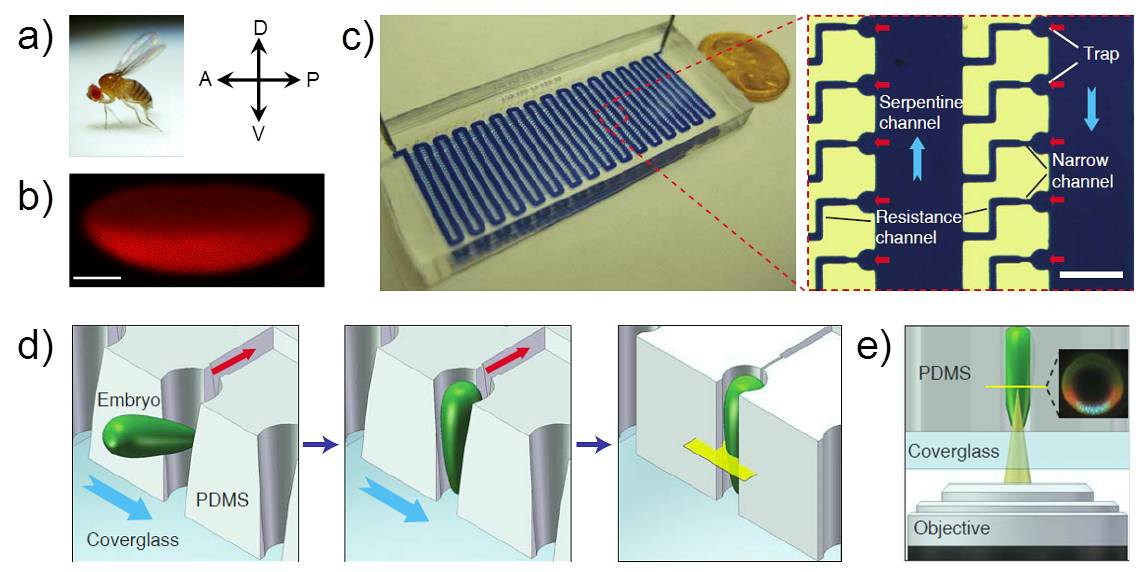
\includegraphics[width=0.65\textwidth]{drosophila_imaging_setup}
\caption{}
\label{subfig:imaging_device}
\end{subfigure}
\begin{subfigure}{0.55\textwidth}
\includegraphics[width=0.8\textwidth]{drosophila_schematic}\\
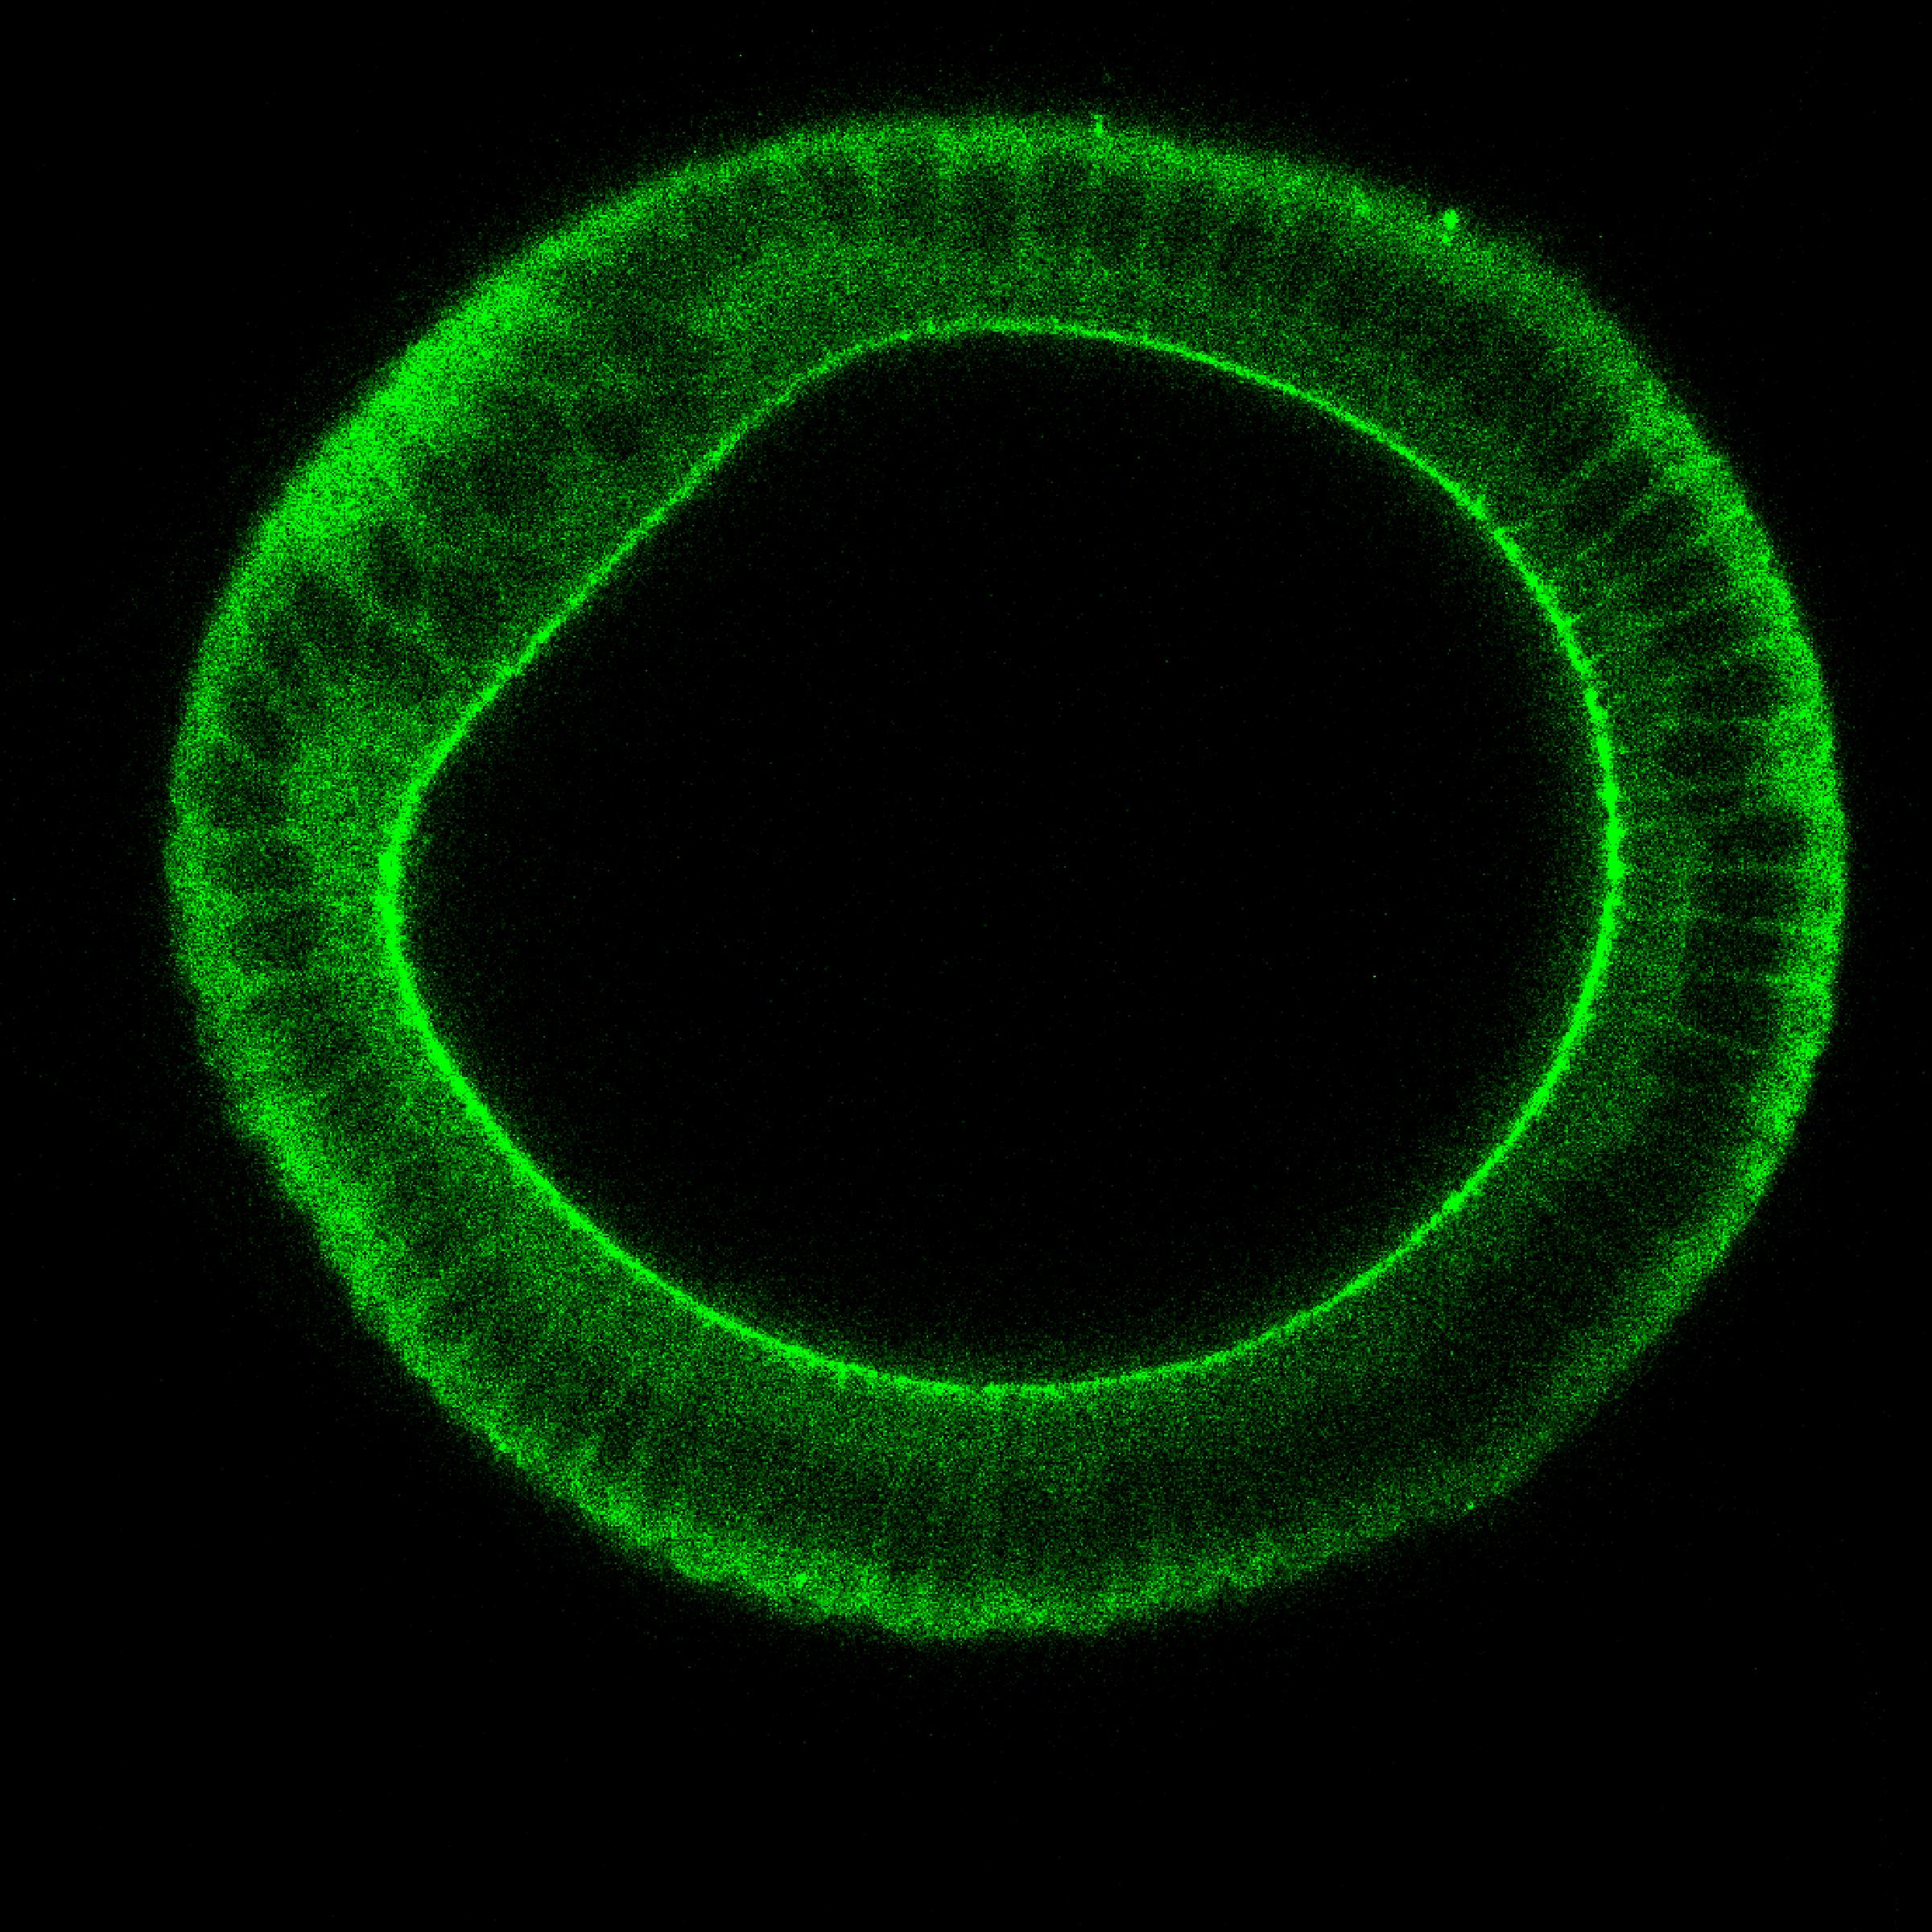
\includegraphics[width=0.3\textwidth]{drosophila_membrane}
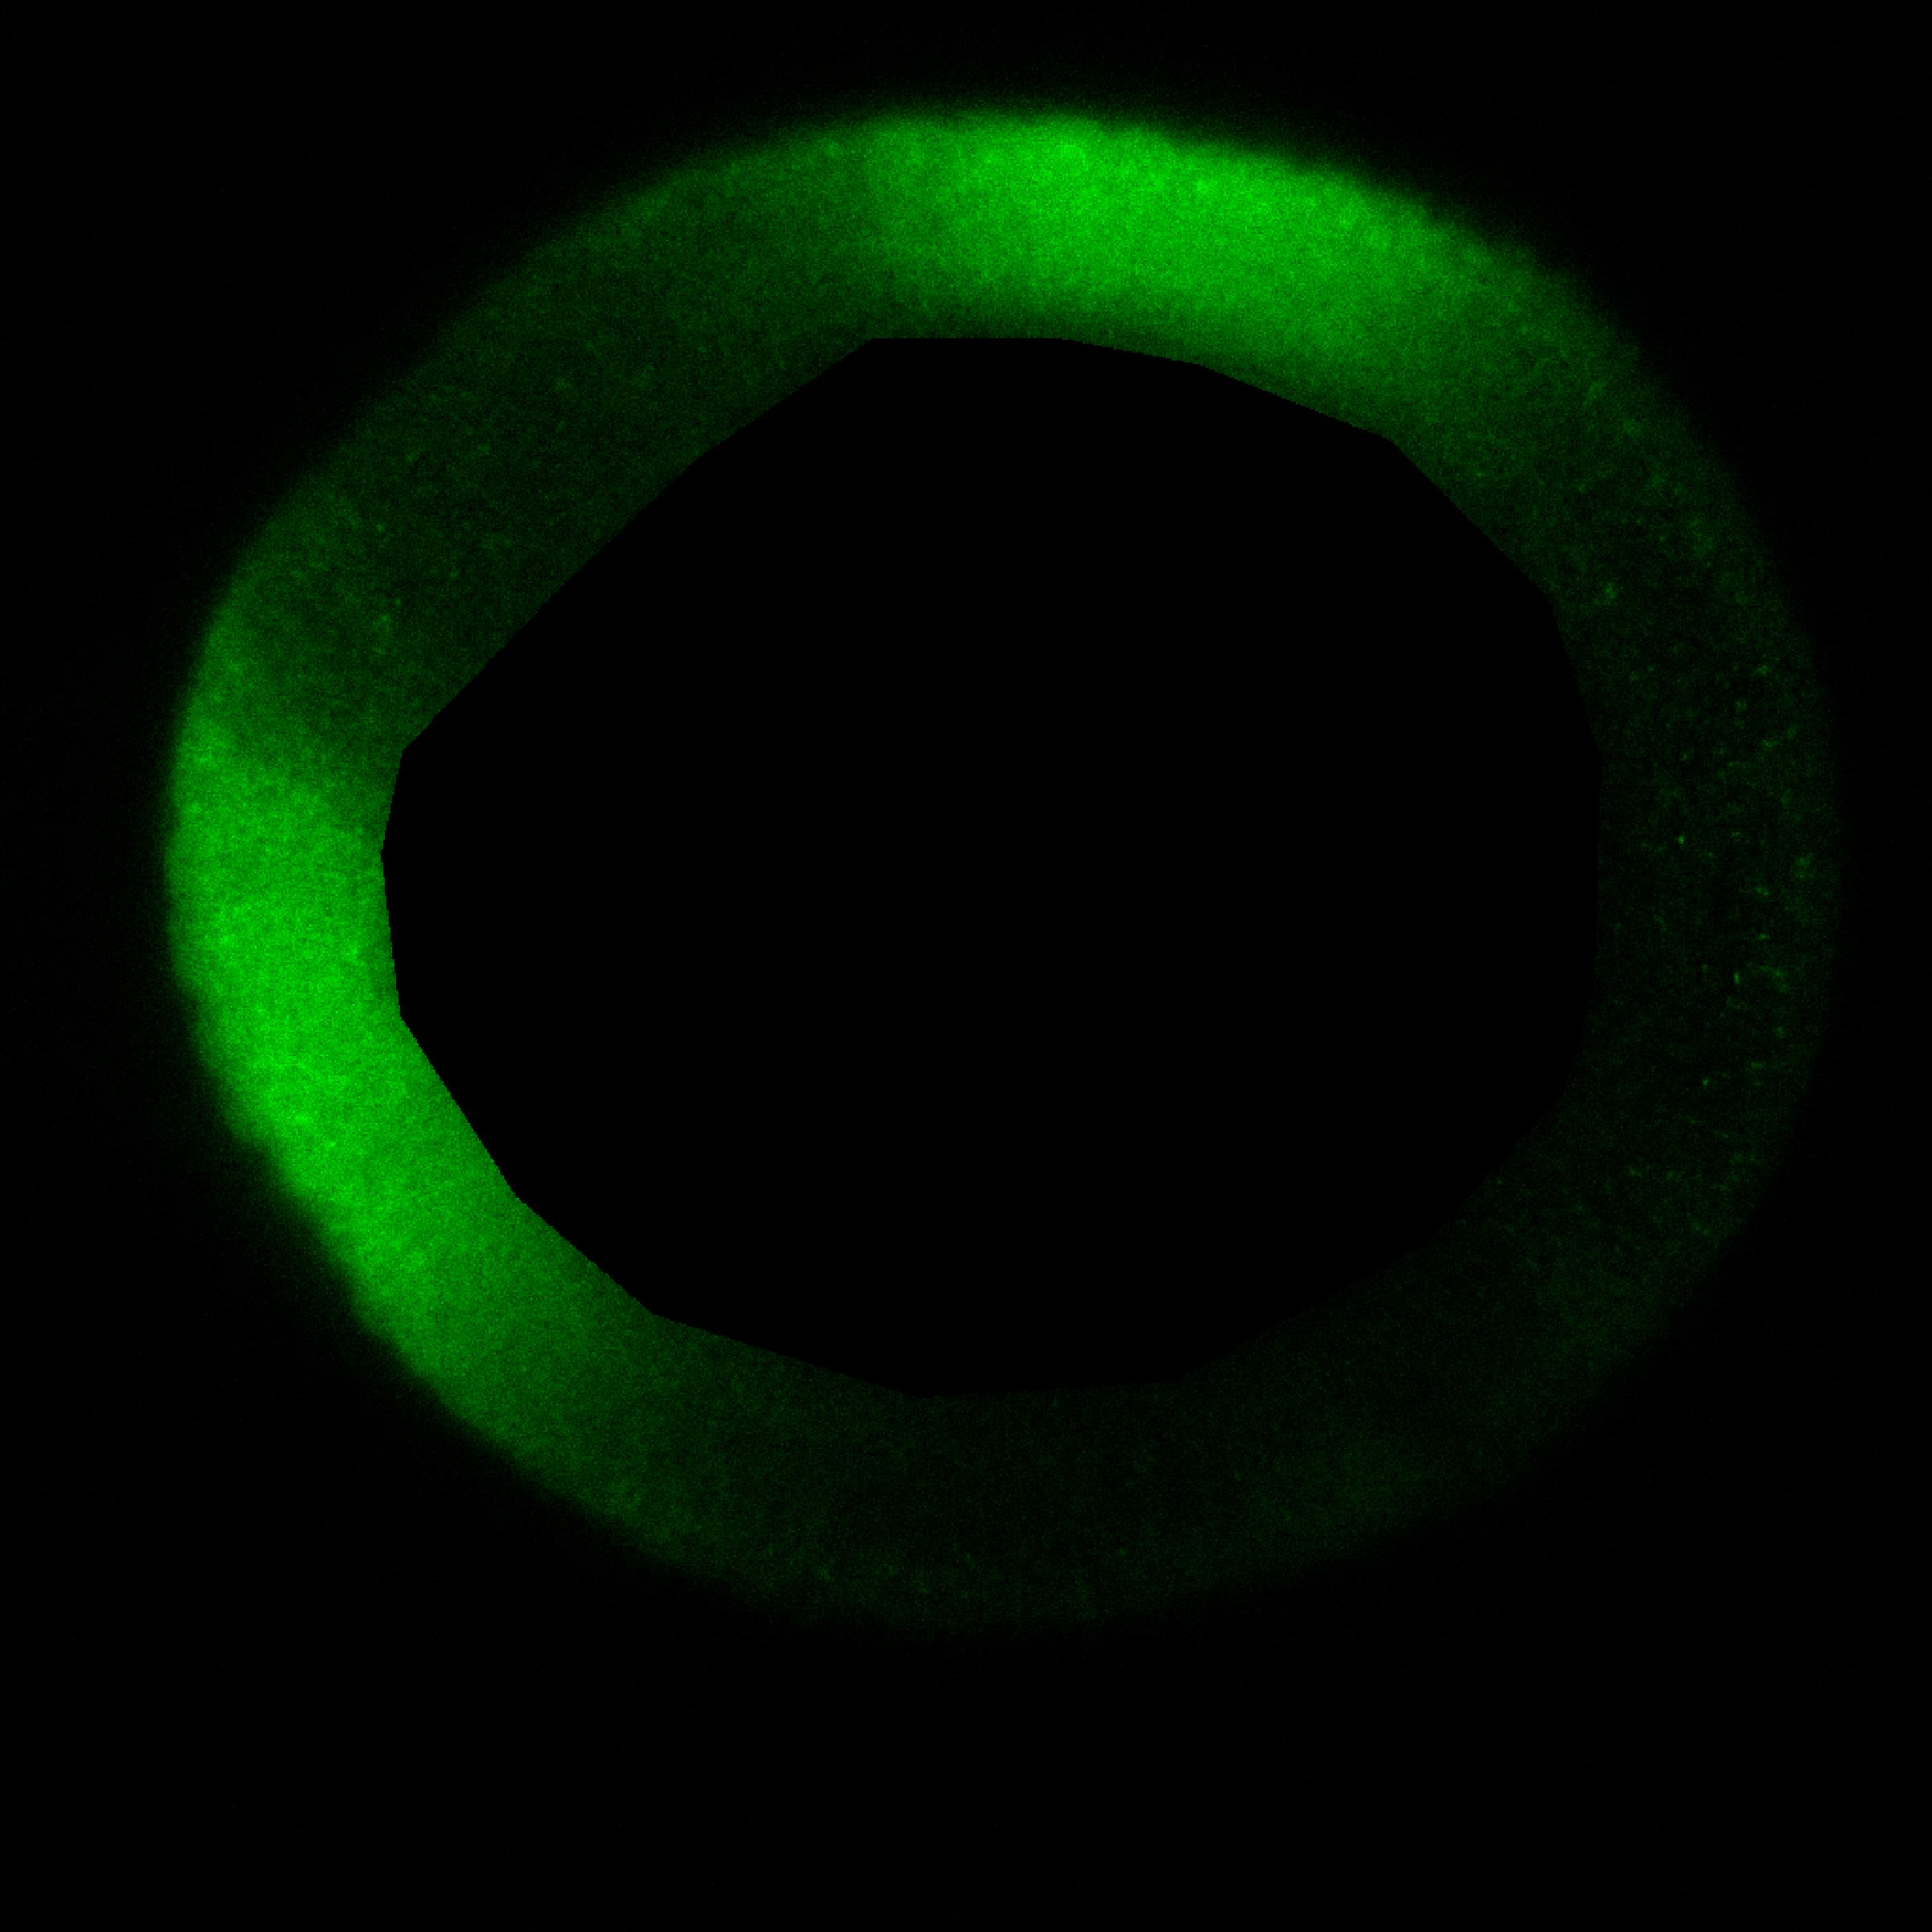
\includegraphics[width=0.3\textwidth]{drosophila_dpERK}
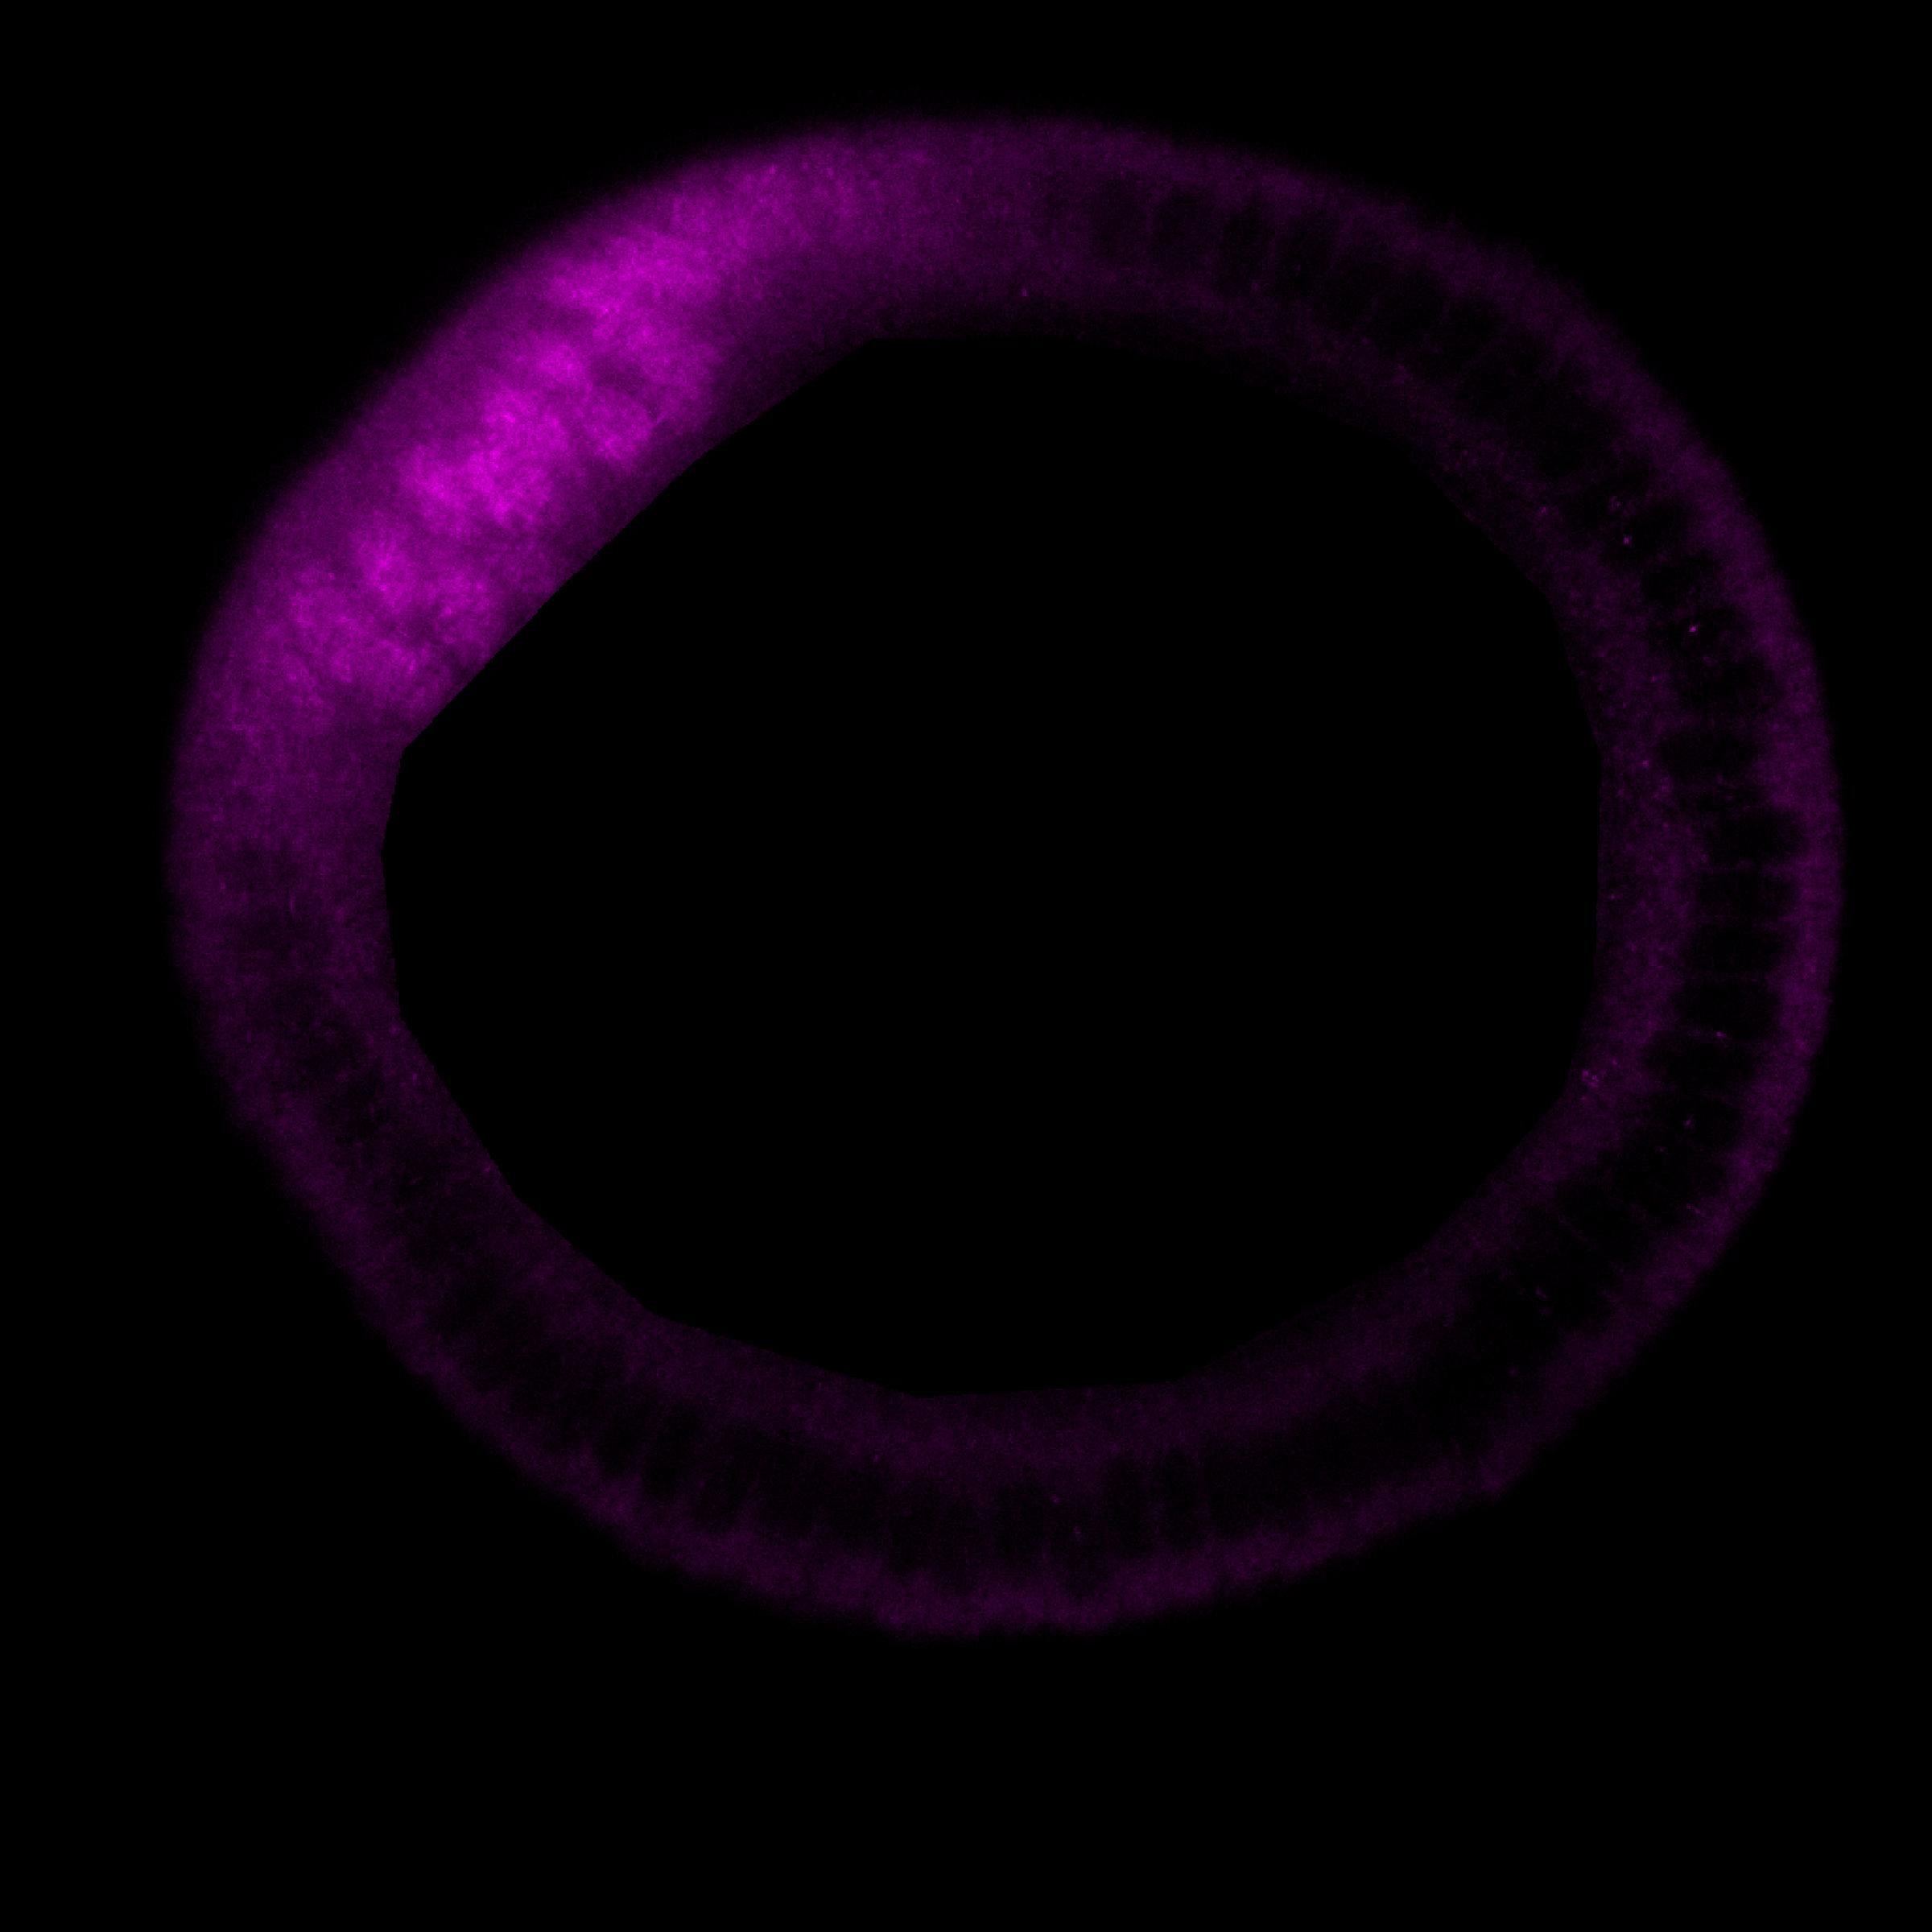
\includegraphics[width=0.3\textwidth]{drosophila_DI}
\caption{}
\end{subfigure}
\begin{subfigure}{0.35\textwidth}
\centering
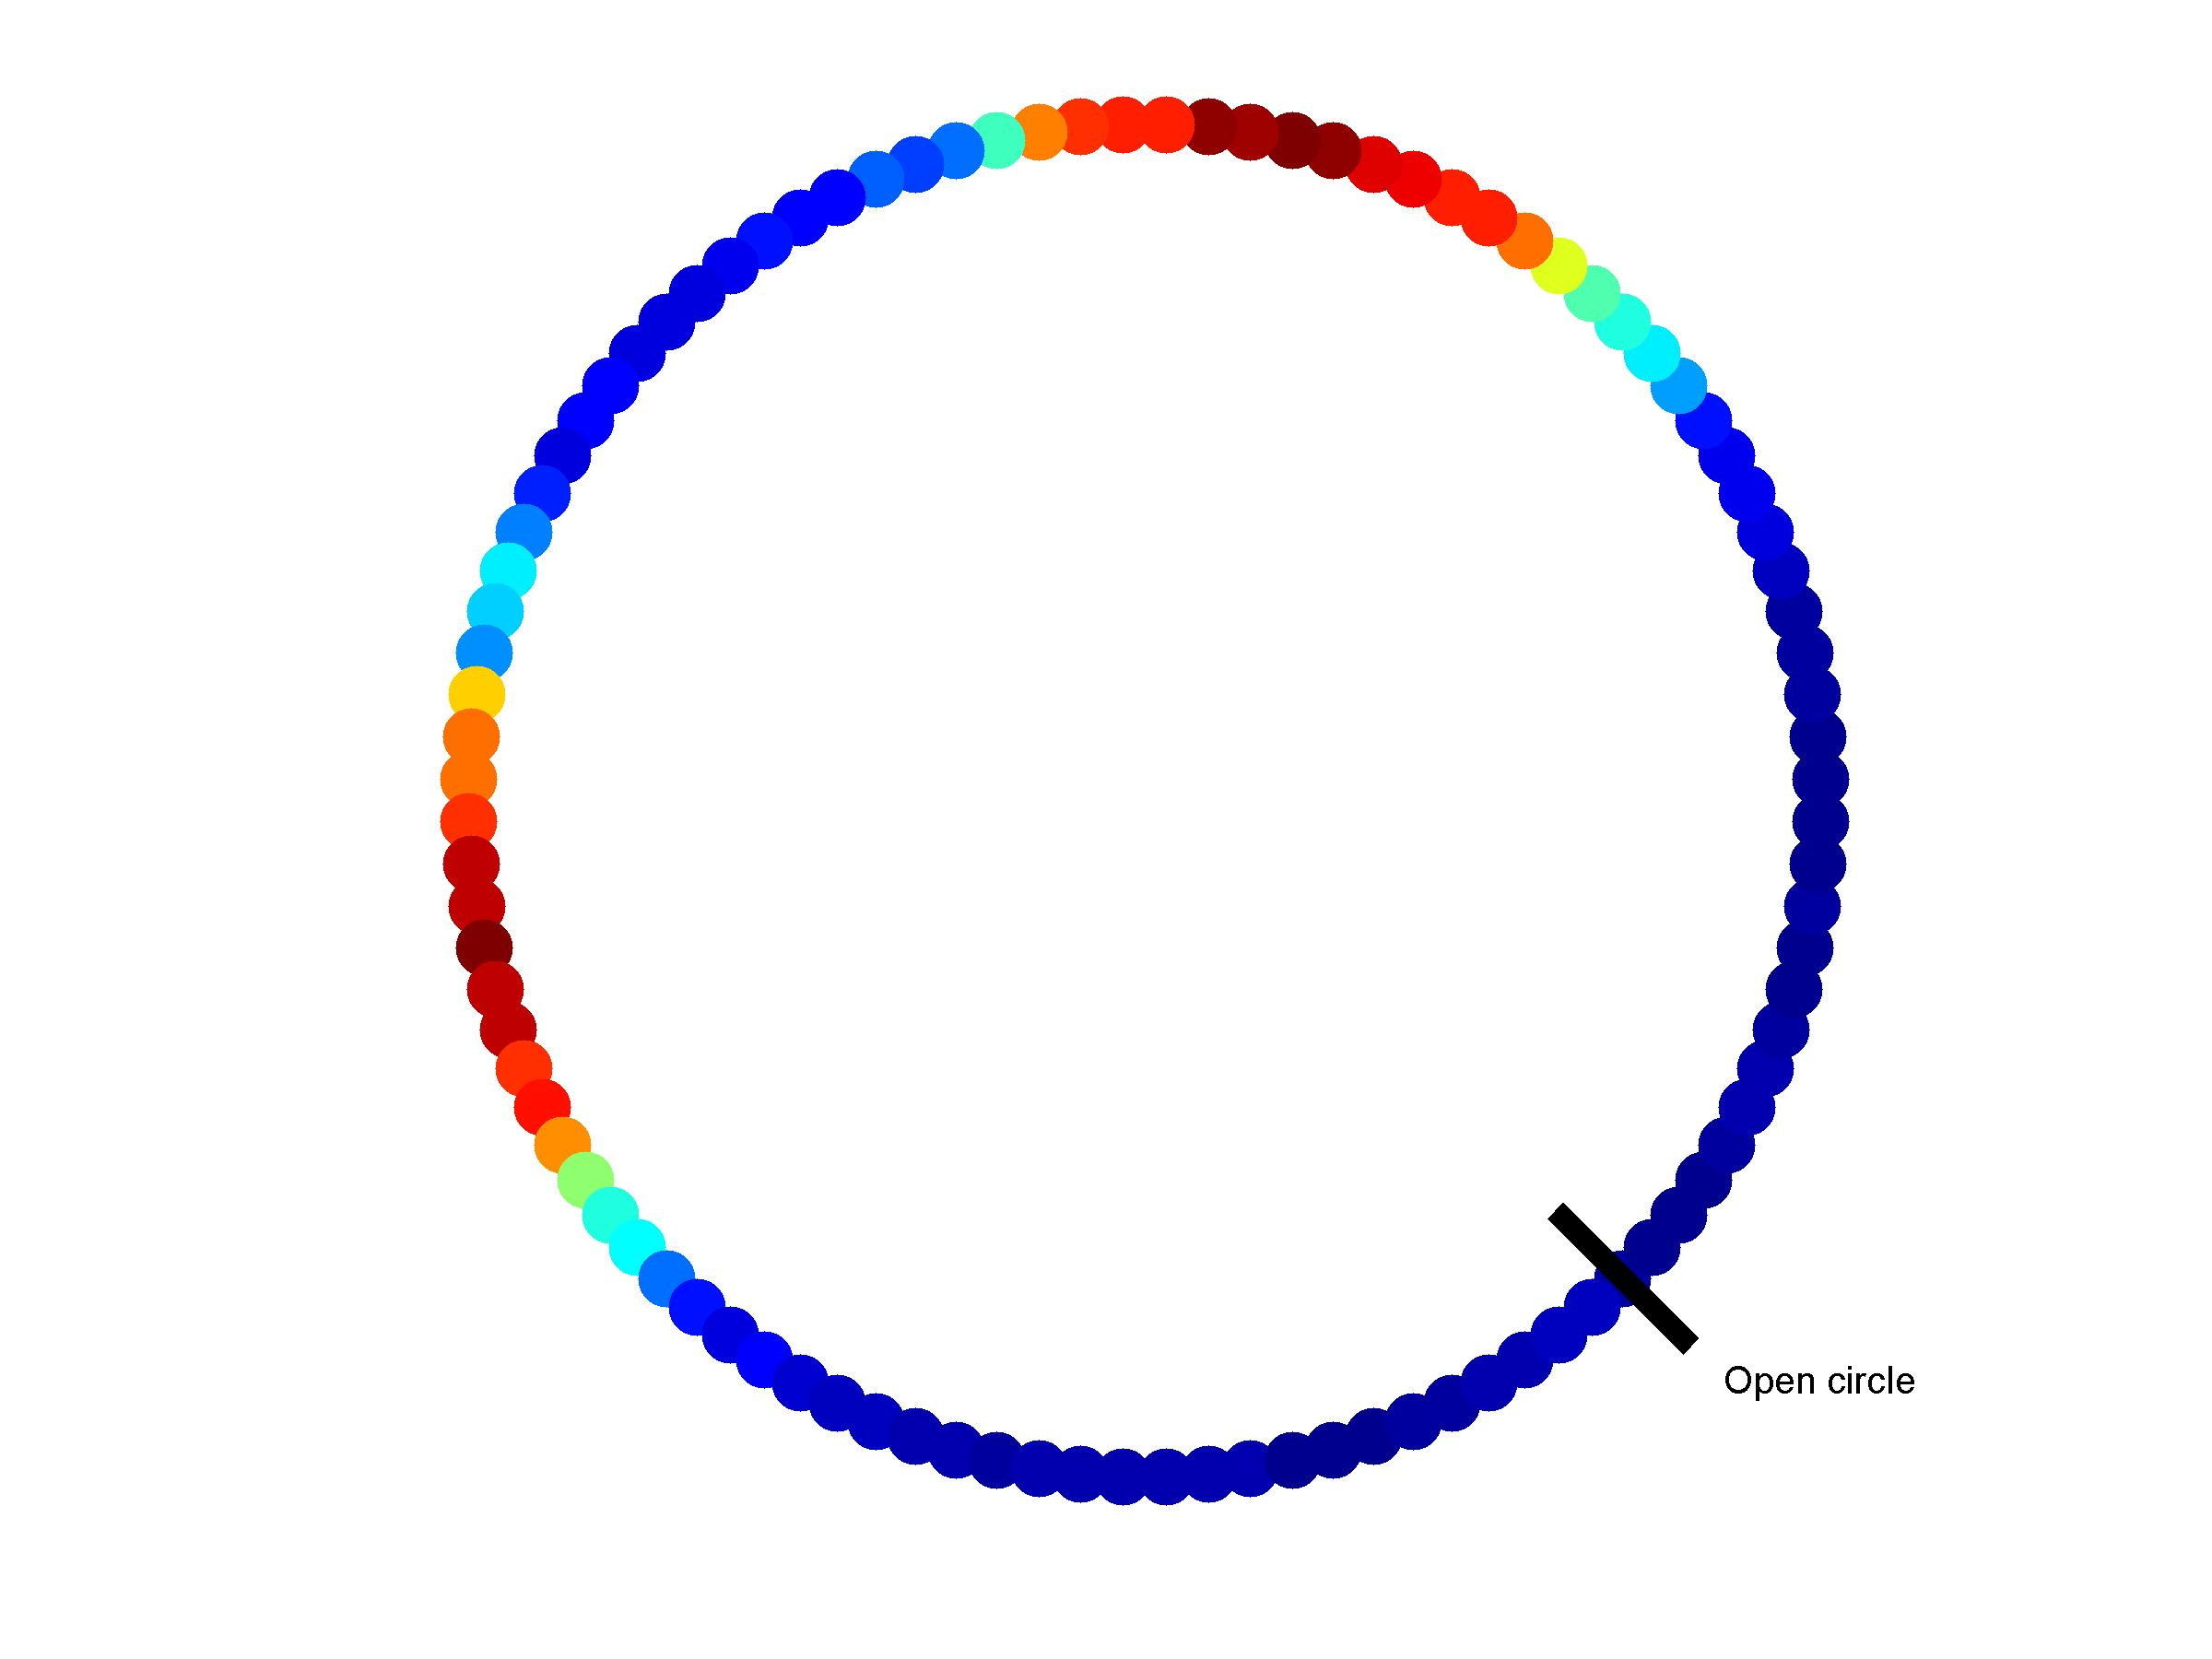
\includegraphics[width=0.6\textwidth]{circle_profile}\\
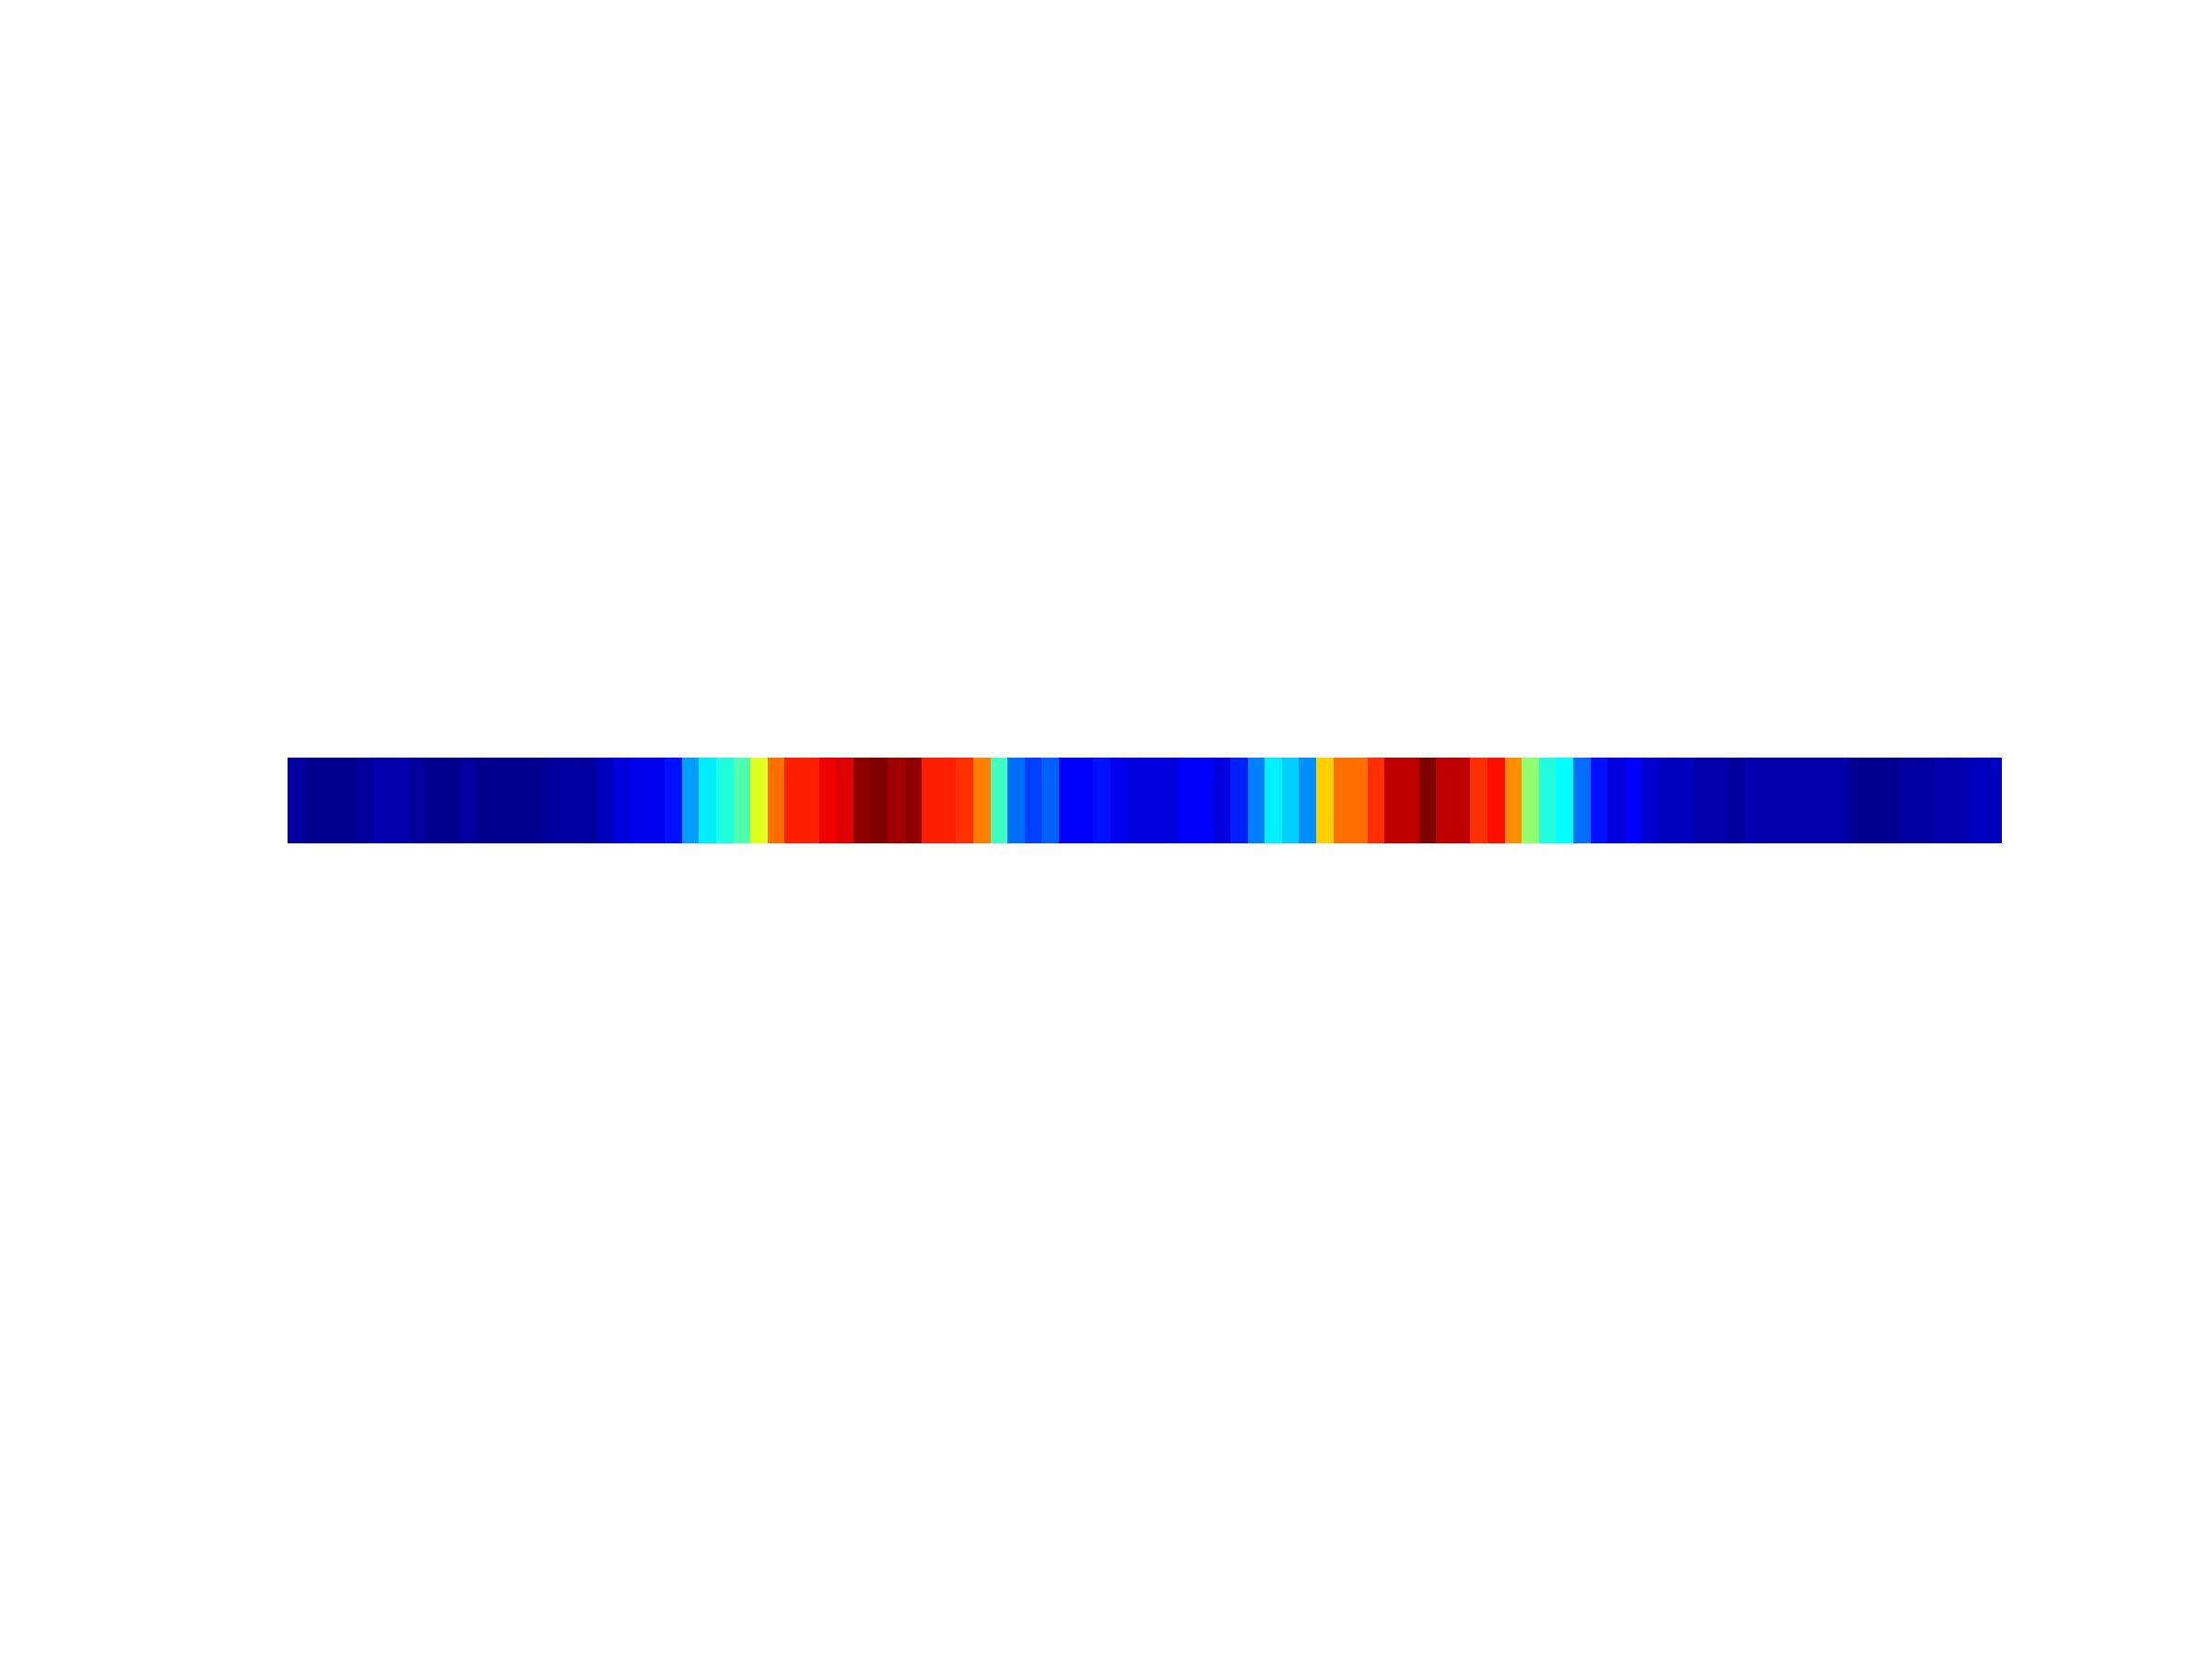
\includegraphics[width=\textwidth, trim=0mm 300mm 0mm 200mm, clip]{line_profile}
\caption{}
\end{subfigure}\\
\begin{subfigure}{0.4\textwidth}
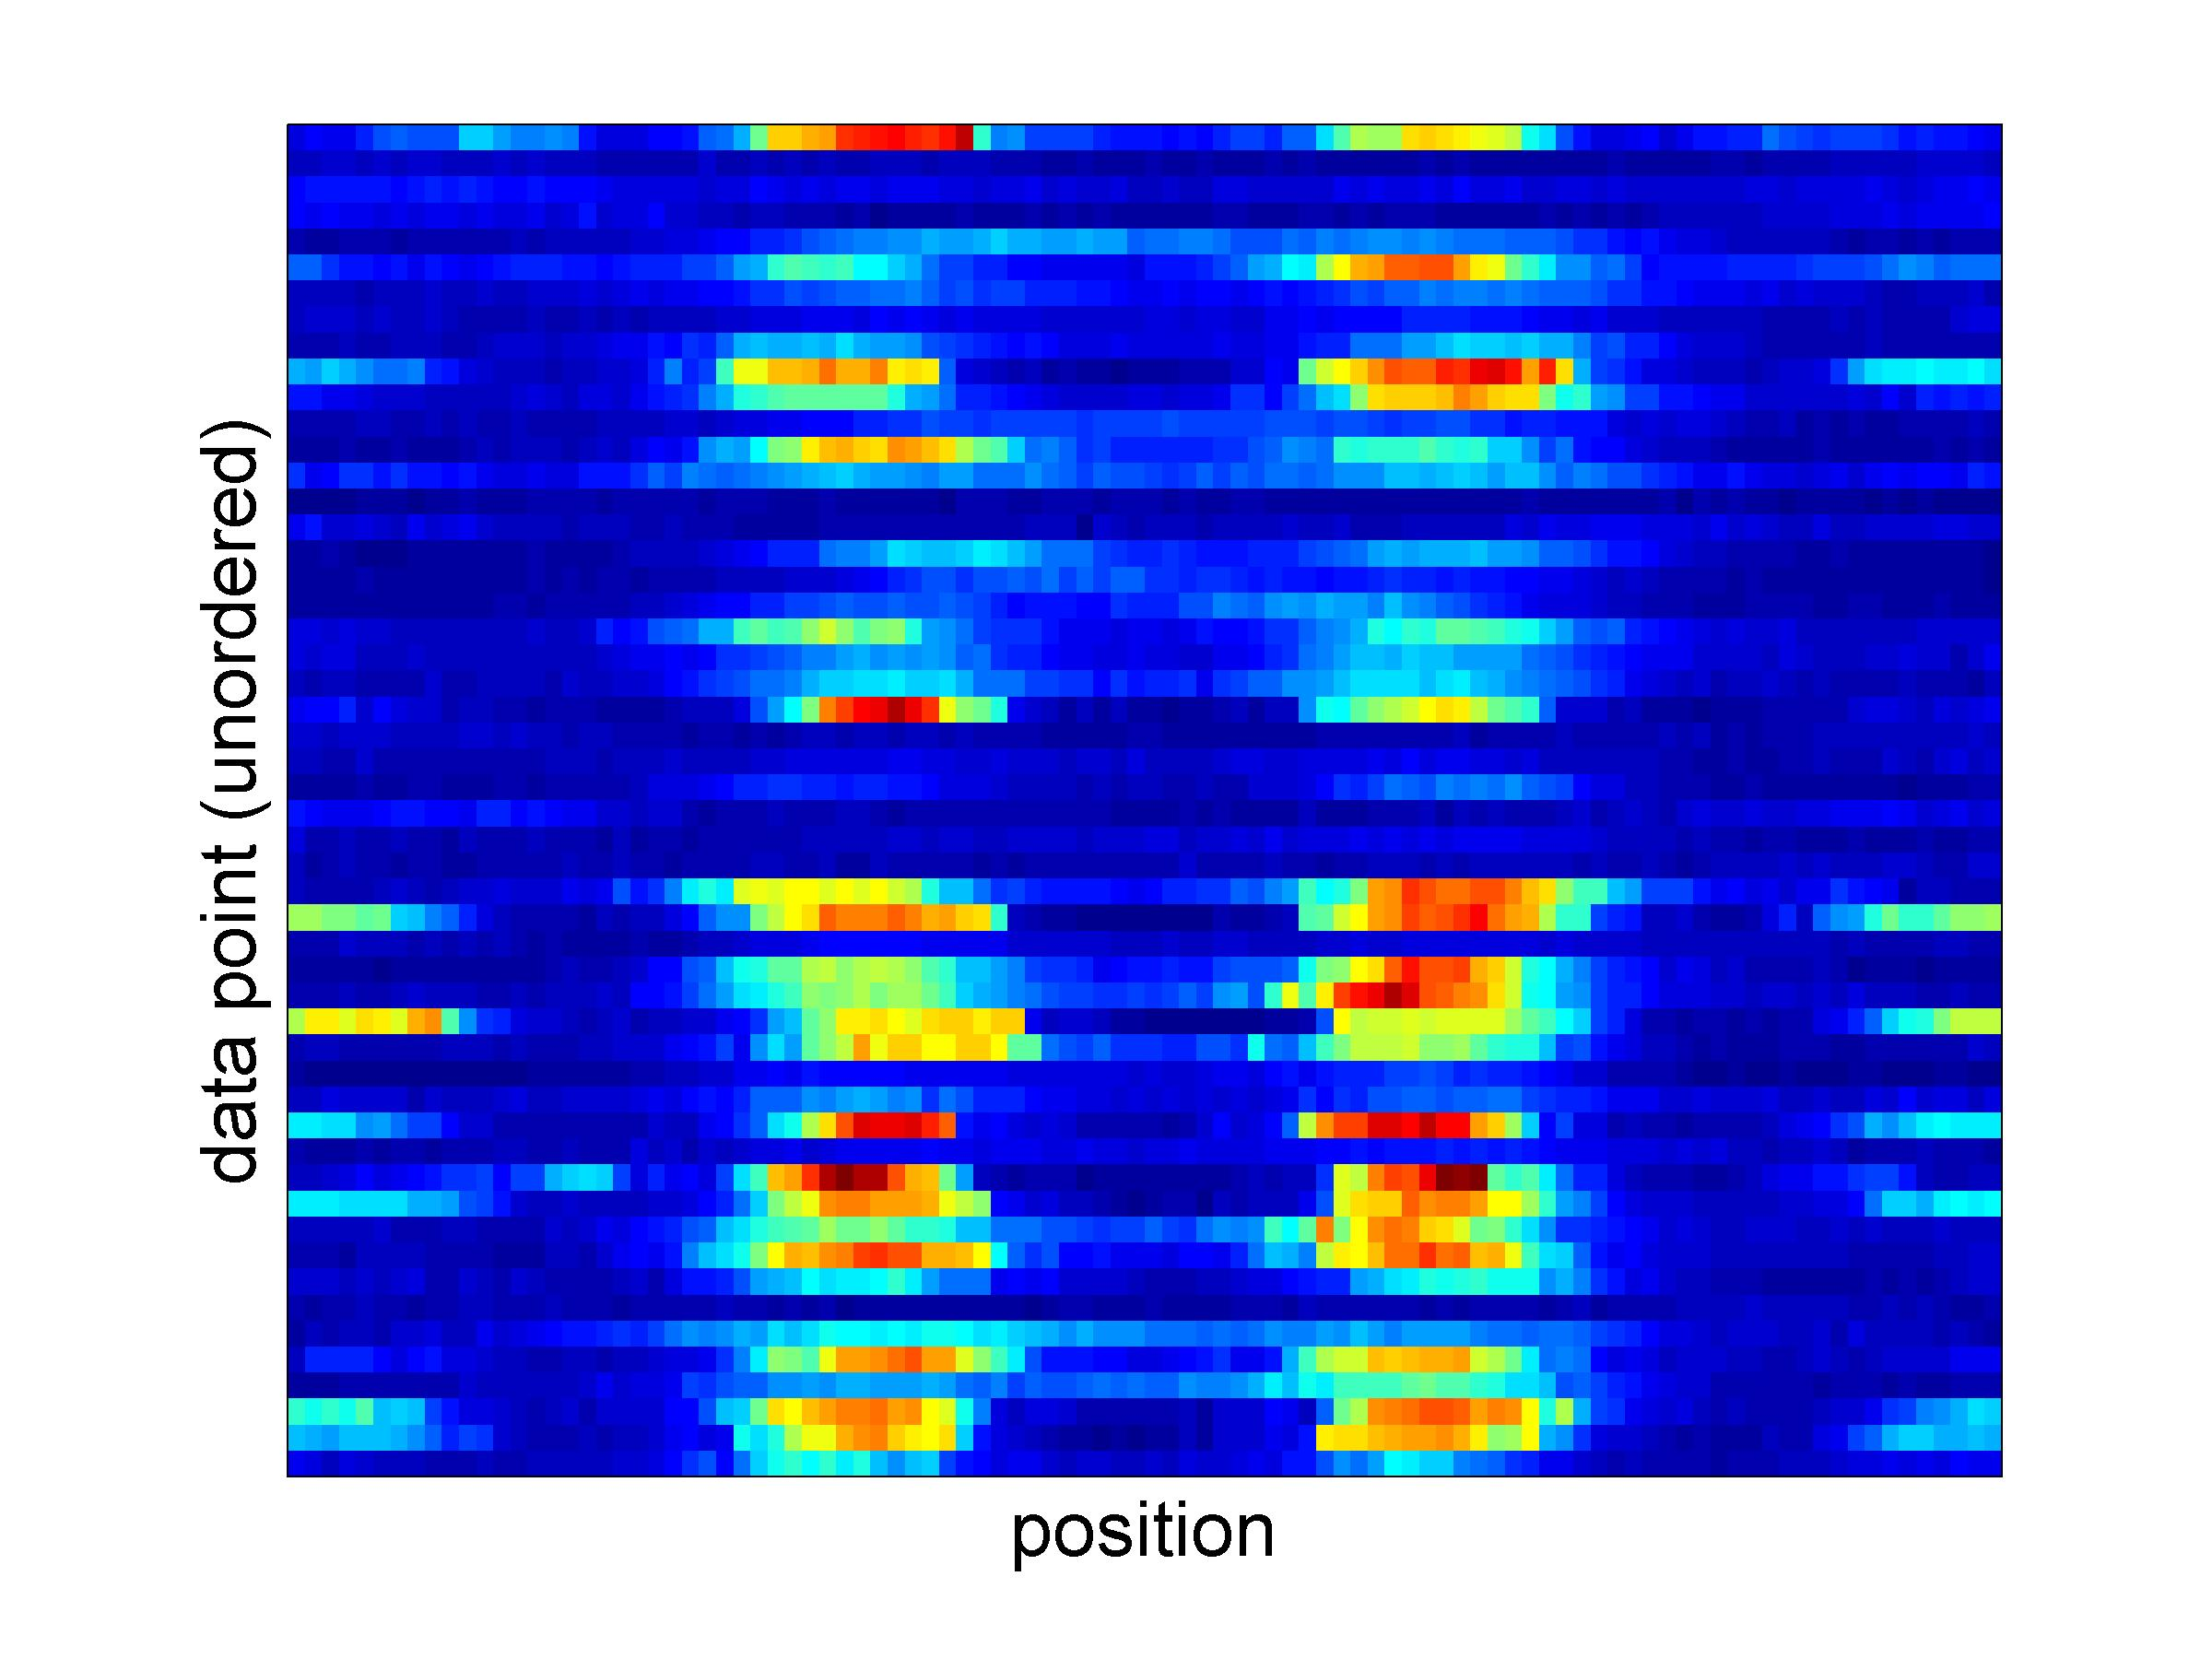
\includegraphics[width=\textwidth]{data_unordered}
\caption{}
\end{subfigure}
\begin{subfigure}{0.4\textwidth}
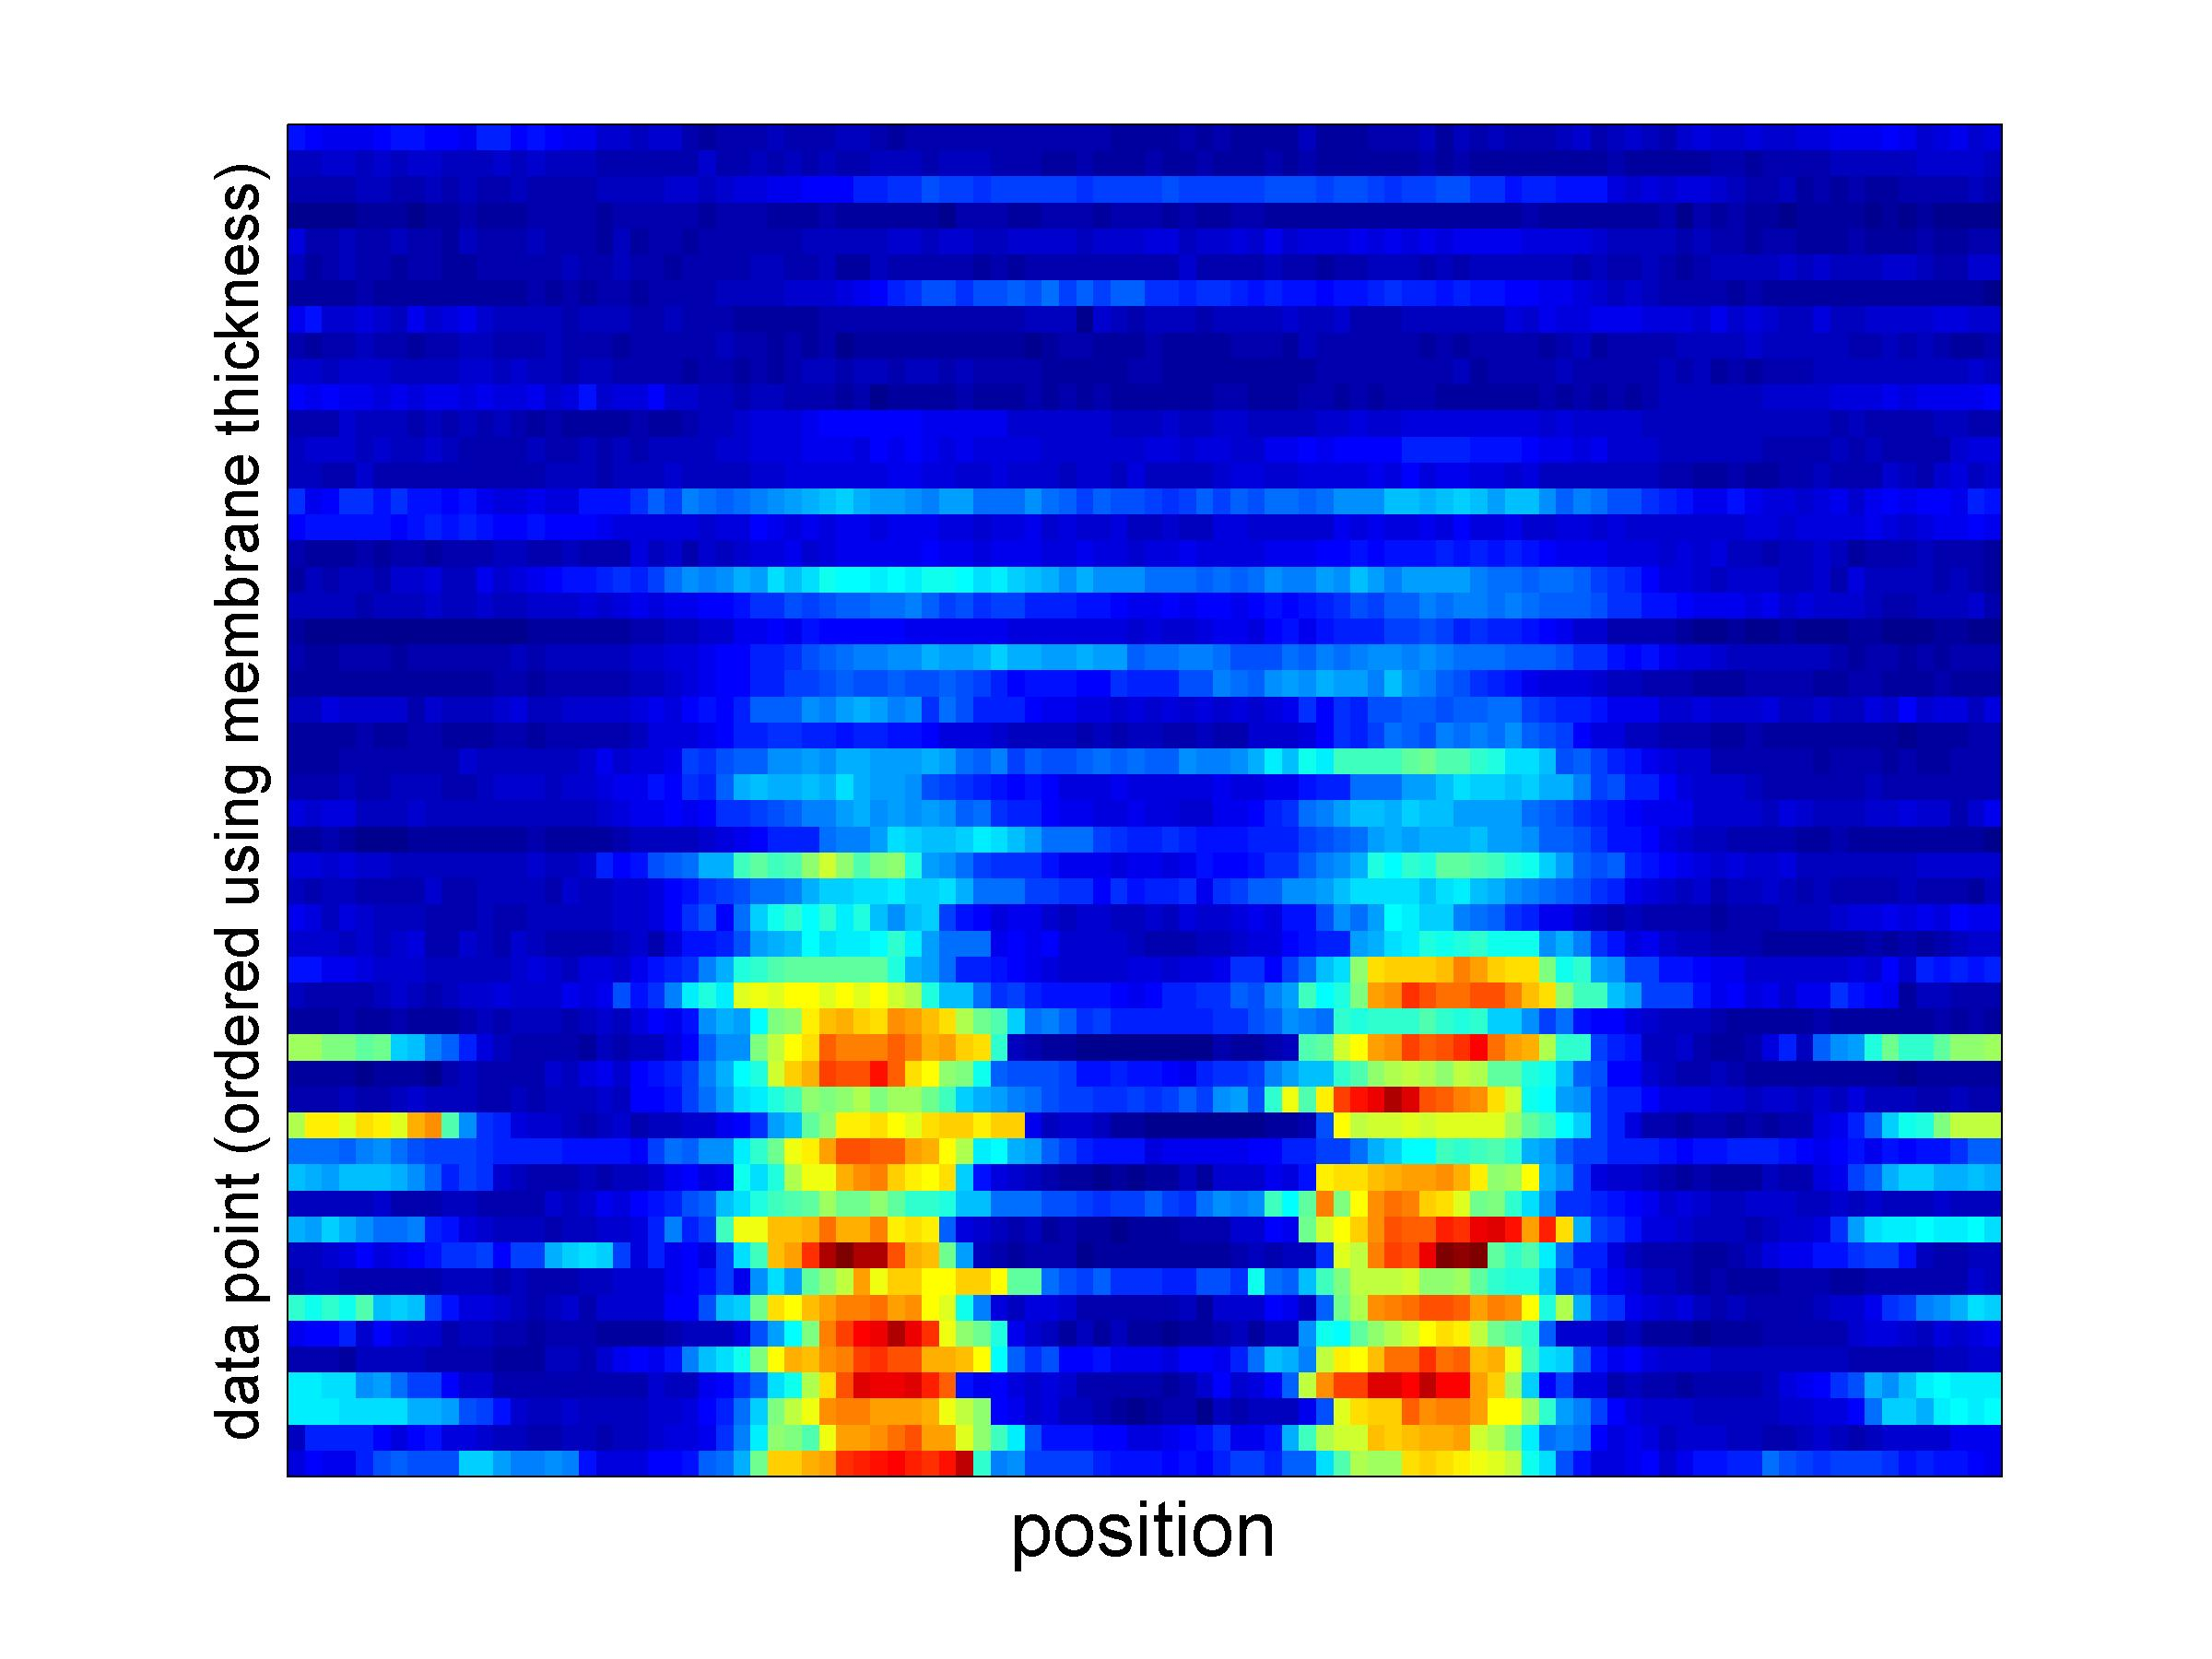
\includegraphics[width=\textwidth]{data_ordered_membrane}
\caption{}
\end{subfigure}
\end{center}
\caption{{\bf Data collection.} (a) Schematic of {\em Drosophila} embryo (longitudinal and cross-section), and cross-sectional fluorescent images of an embryo stained for the membrane proteins (left), dpERK (center), and dorsal protein (right).
(b) Concentration profile of dpERK extracted from a fluorescent image. The circular profile is ``unwrapped'' at the dorsal midline (determined from the expression of the dorsal protein) to obtain a concentration profile on a line.
(c) Concentration profiles of dpERK for many embryos. Each row represents a different embryo fixed at a slightly different developmental time.
(d) Concentration profiles of dpERK for many embryos from (c), now ordered by the thickness of the membrane. The membrane thickness is known to be one-to-one with time.}
\label{fig:background}
\end{figure}

Here,  we will discuss alternative methodologies to reconstruct the dpERK dynamics from fluorescent images. 
%
We will use various data mining techniques to {\em automatically} order the dpERK concentration profiles in time.
%
We will not only focus on the linear concentration profiles extracted from the images, but also work directly with the two-dimensional dpERK fluorescent images. 
%
Finally, we will look at ordering the two-dimensional membrane images in time; these are much more feature-rich than the dpERK images, and prove to be more challenging.

% Results and Discussion can be combined.
\section*{Results}

\subsection*{dpERK concentration profiles ordered using principal component analysis}

We first used Principal Components Analysis (PCA) to automatically order the one-dimensional concentration profiles in time. 
%
We computed the first principal component, $\psi_1$, from the data set, and ordered the data by the projection coefficients onto $\psi_1$. 
%
The results are shown in Figure \ref{fig:PCA_ordering}.
%
There is a strong correlation between the first projection coefficient, $\langle x_i, \psi_1 \rangle$, and the membrane thickness.

\begin{figure}[H]
\begin{subfigure}{0.3\textwidth}
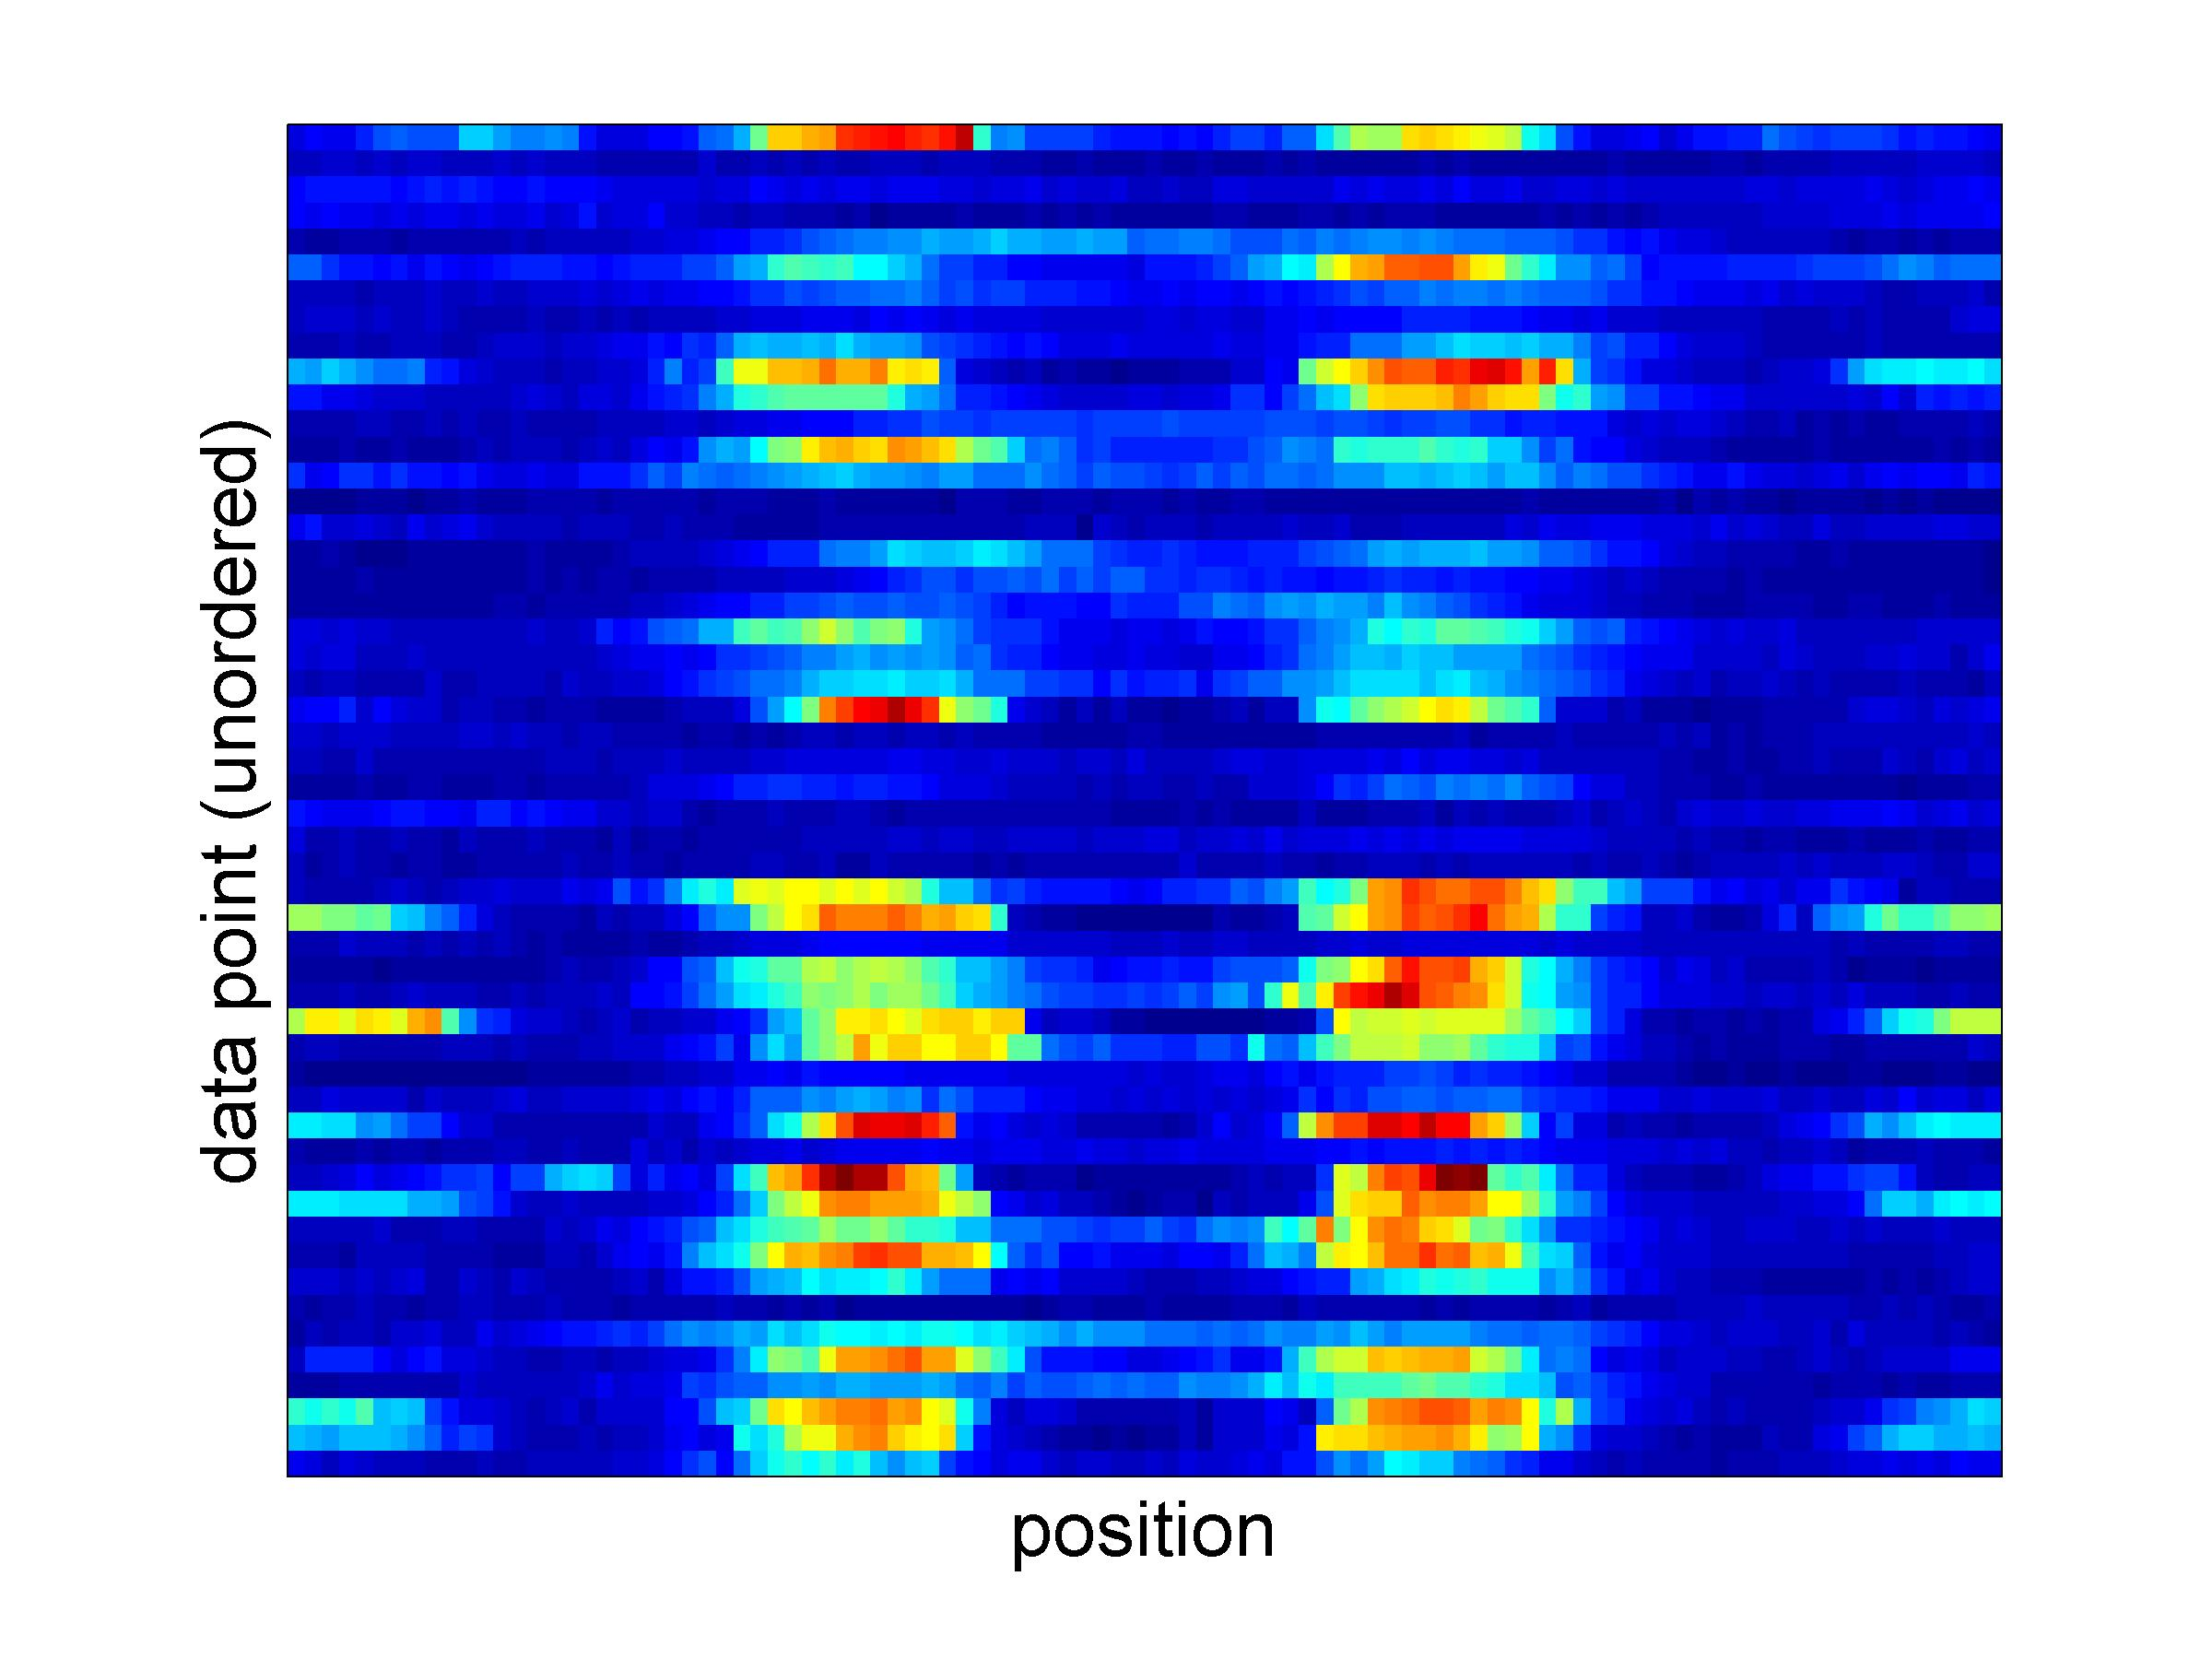
\includegraphics[width=\textwidth]{data_unordered}
\caption{}
\label{subfig:unordered_profiles}
\end{subfigure}
\begin{subfigure}{0.3\textwidth}
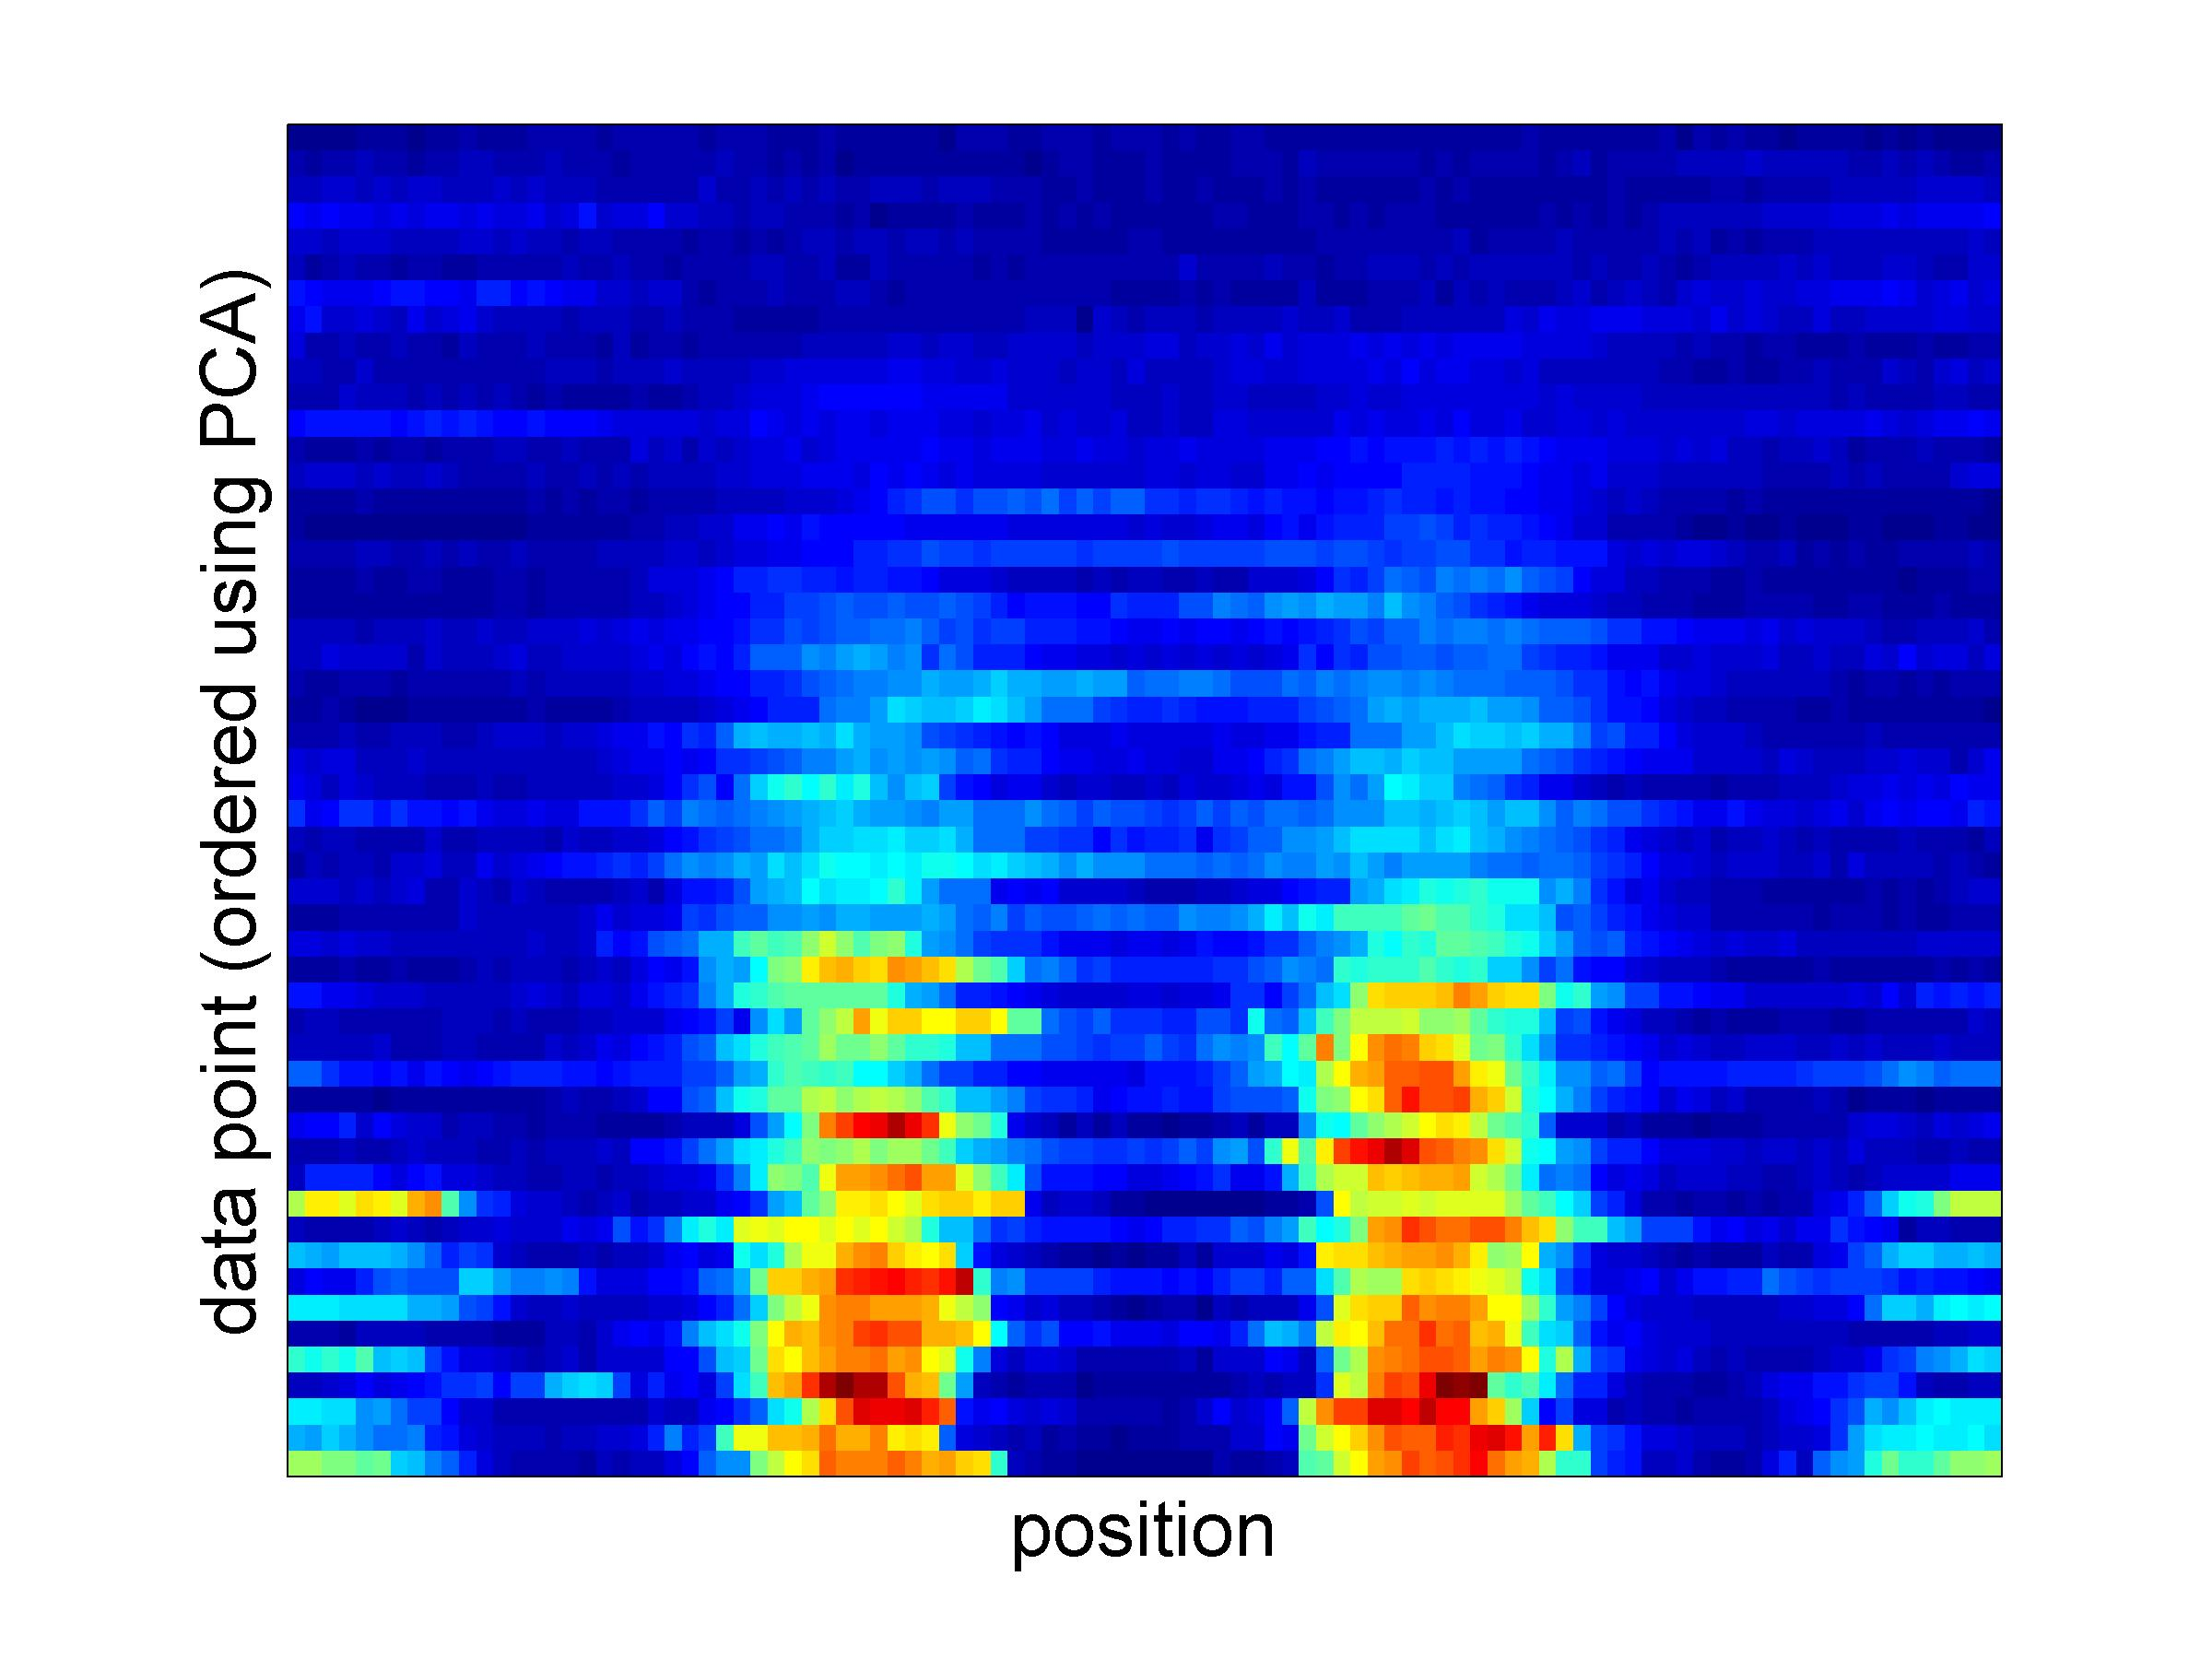
\includegraphics[width=\textwidth]{data_ordered_PCA}
\caption{}
\label{subfig:PCA_ordering_image}
\end{subfigure}
\begin{subfigure}{0.3\textwidth}
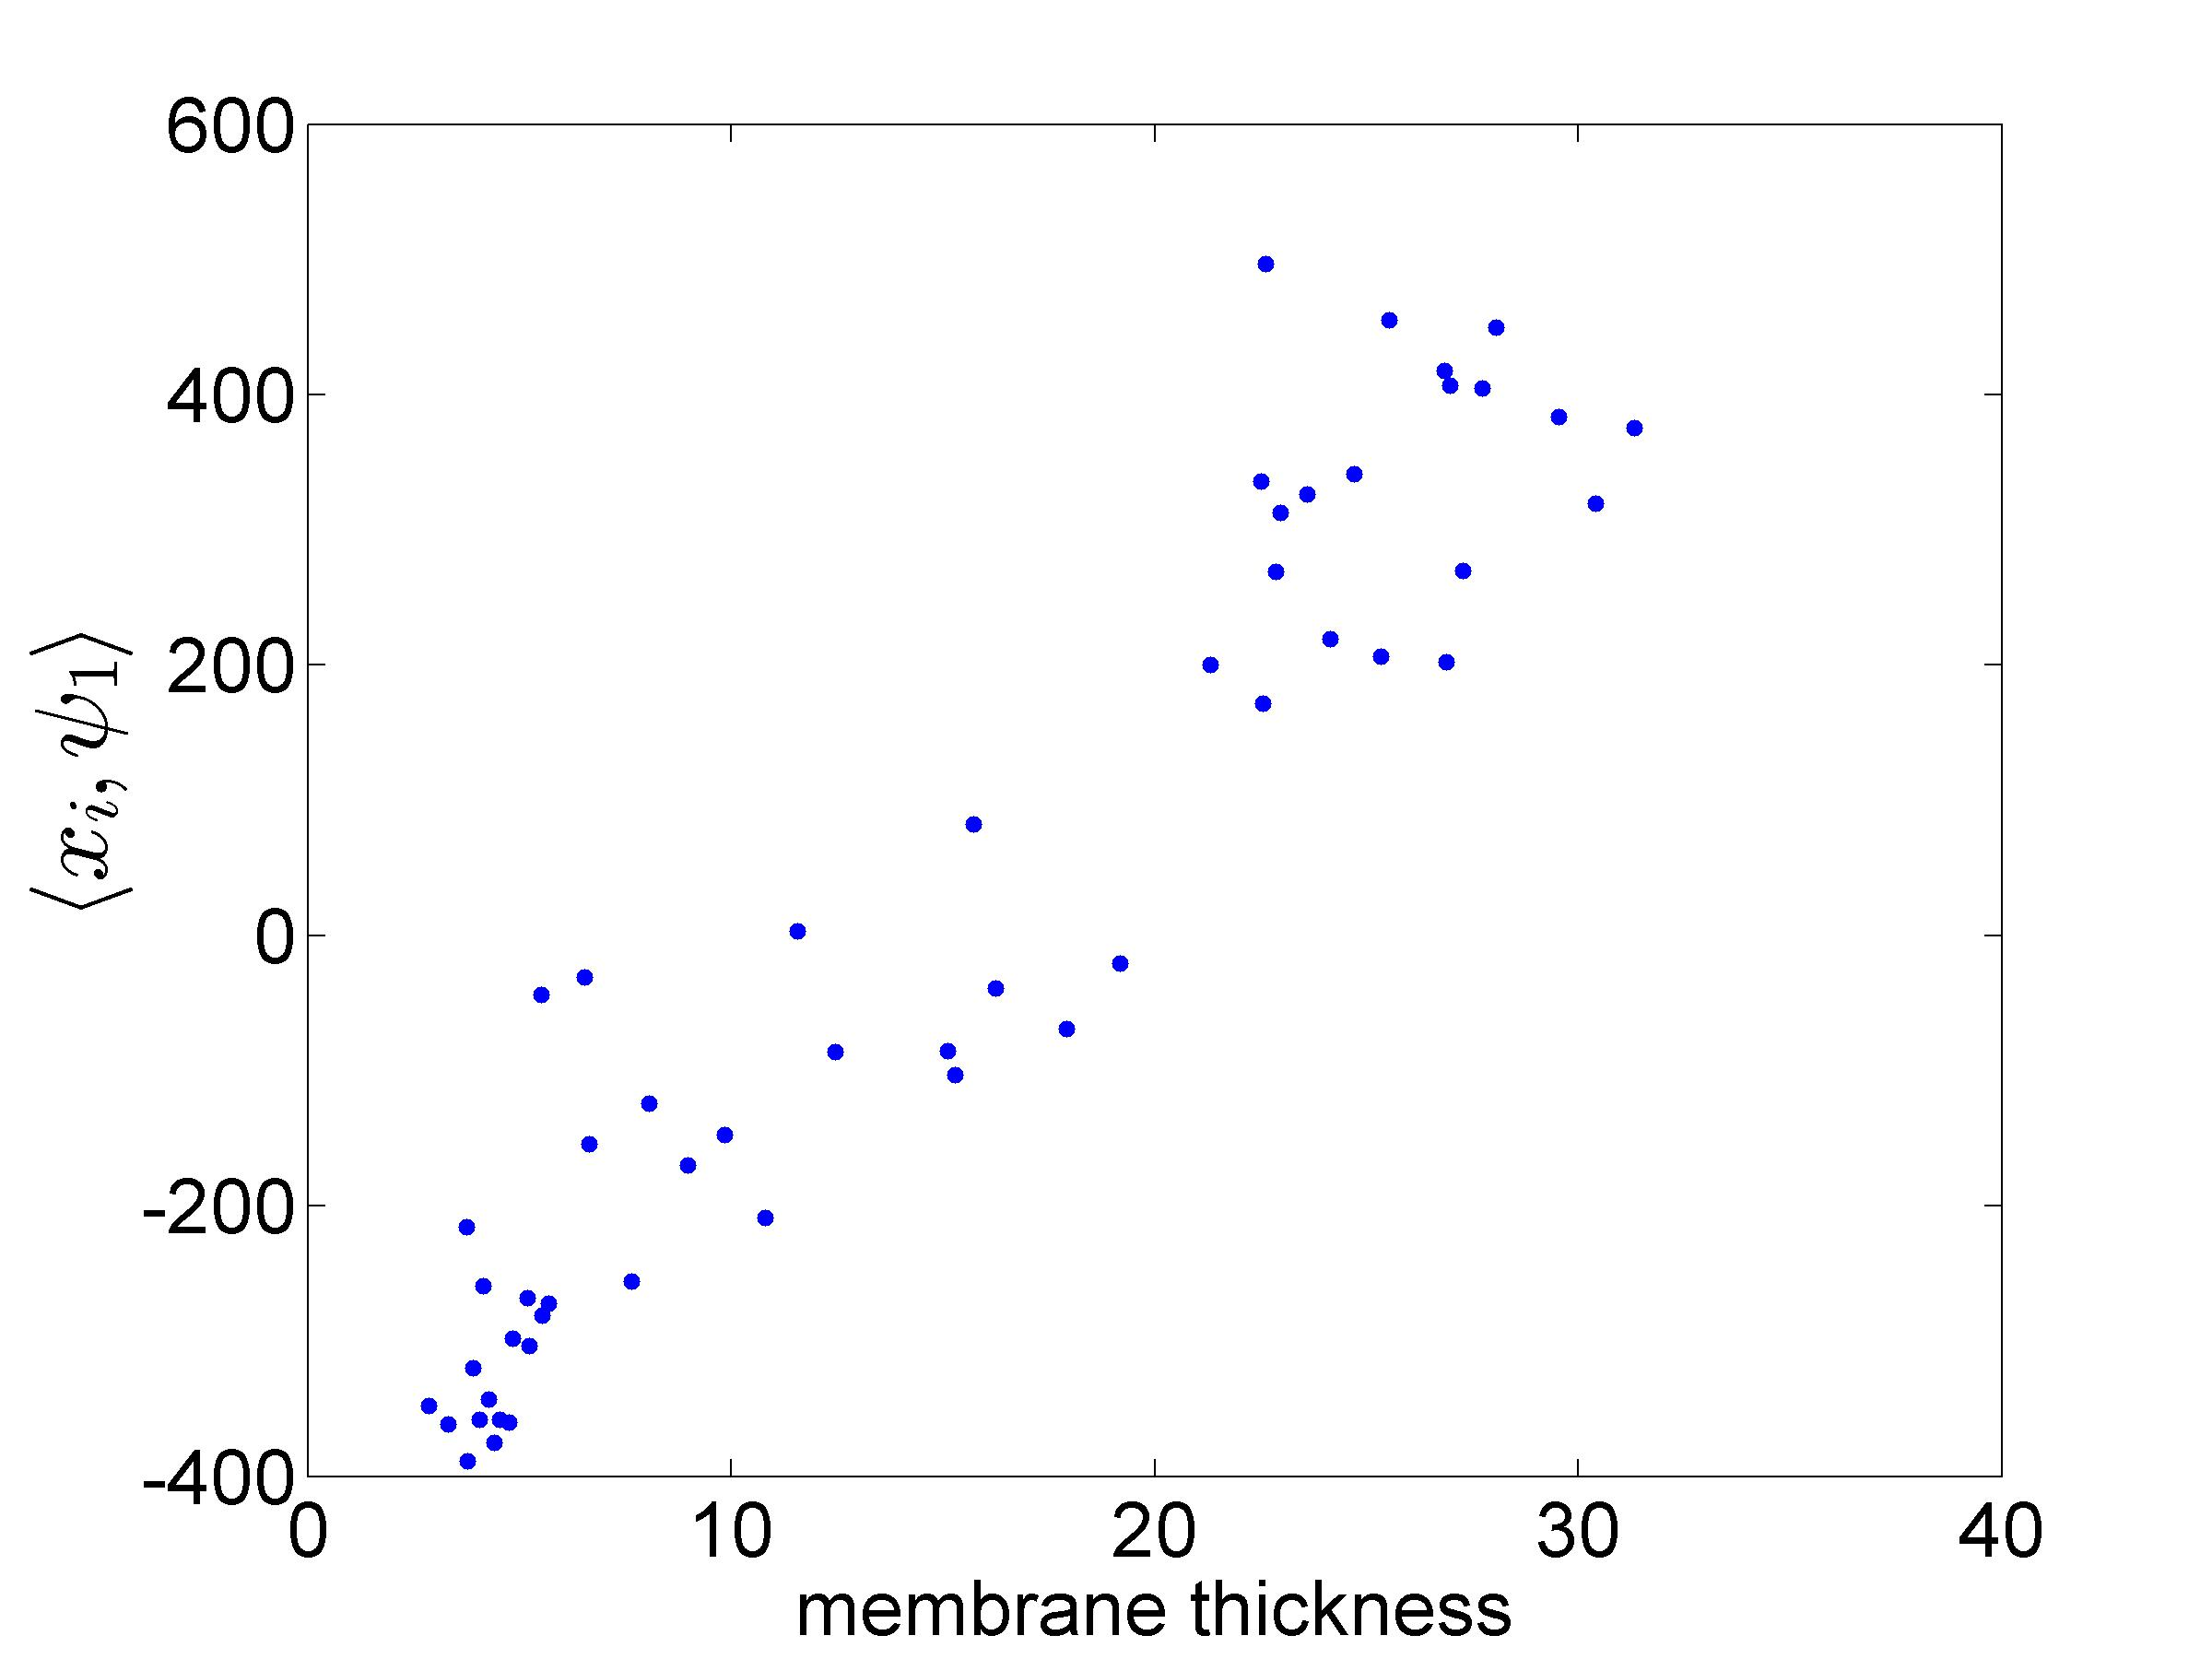
\includegraphics[width=\textwidth]{PCA_time_corr}
\caption{}
\end{subfigure}
\caption{{\bf Ordering dpERK concentration profiles using PCA.} (a) Concentration profiles of dpERK for many embryos. Each row represents a different embryo fixed at a slightly different developmental time.
(b) Concentration profiles of dpERK from (a), now ordered by the first PCA projection coefficient.
(c) Correlation between the first PCA projection coefficient and the membrane thickness.}
\label{fig:PCA_ordering}
\end{figure}

We would like to note that, because the embryos can be oriented with either the anterior or posterior end facing up in the microfluidic device (see Figure \ref{subfig:imaging_device}), the directionality of the concentration profiles (clockwise versus counterclockwise around the ring, or right-to-left versus left-to-right for the linear profiles) is not meaningful. 
%
Therefore, we could also do PCA with an expanded data set where we also include the mirror image of each concentration profile.
%
Symmetries in PCA have been studied extensively in previous work \cite{holmes1998turbulence}; it was shown that when mirror images are also included in the data set, the first PCA mode captures the symmetric portion of the variability, and the second mode captures the anti-symmetric portion.
%
We found that including the mirror images of each data point did not change our results significantly, since the first principal component (not shown) is nearly symmetric with respect to left-right reflections.

\subsection*{dpERK concentration profiles ordered using diffusion maps}

Although PCA was rather successful in ordering the concentration profiles, there are some inconsistencies in the orderings.
%
Perhaps the most obvious feature to note is the scrambling of the secondary *ADD NAME* peaks located at the far left and right edges of the concentration profiles.
%
It is known that these peaks arise later in the development of {\em Drosophila};
however, one can see in Figure \ref{subfig:PCA_ordering_image} that these secondary peaks are scrambled when the data is ordered using PCA.
%
We can gain insight into this ``scrambling'' by looking at the projection of the data onto the first two principal components, shown in Figure \ref{subfig:PCA_12}.
%
The data falls onto a one-dimensional {\em nonlinear} curve in this two-dimensional space, implying that nonlinear dimensionality reduction techniques may be more approproate, as they can order the data along the curve, and not simply along the first principal axis.

We chose to use diffusion maps (DMAPS) as our nonlinear dimensionality reduction technique.
%
We computed the diffusion maps embedding for our data set, using the Euclidean distance between concentration profiles as our distance metric.
%
We then ordered the data using the first (nontrivial) diffusion maps coordinate $\phi_2$. 
%
The results are shown in Figure \ref{fig:DMAPS_ordering}.
%
The secondary peaks are now nicely clustered towards the end of the developmental trajectory.

\begin{figure}[H]
\begin{subfigure}{0.3\textwidth}
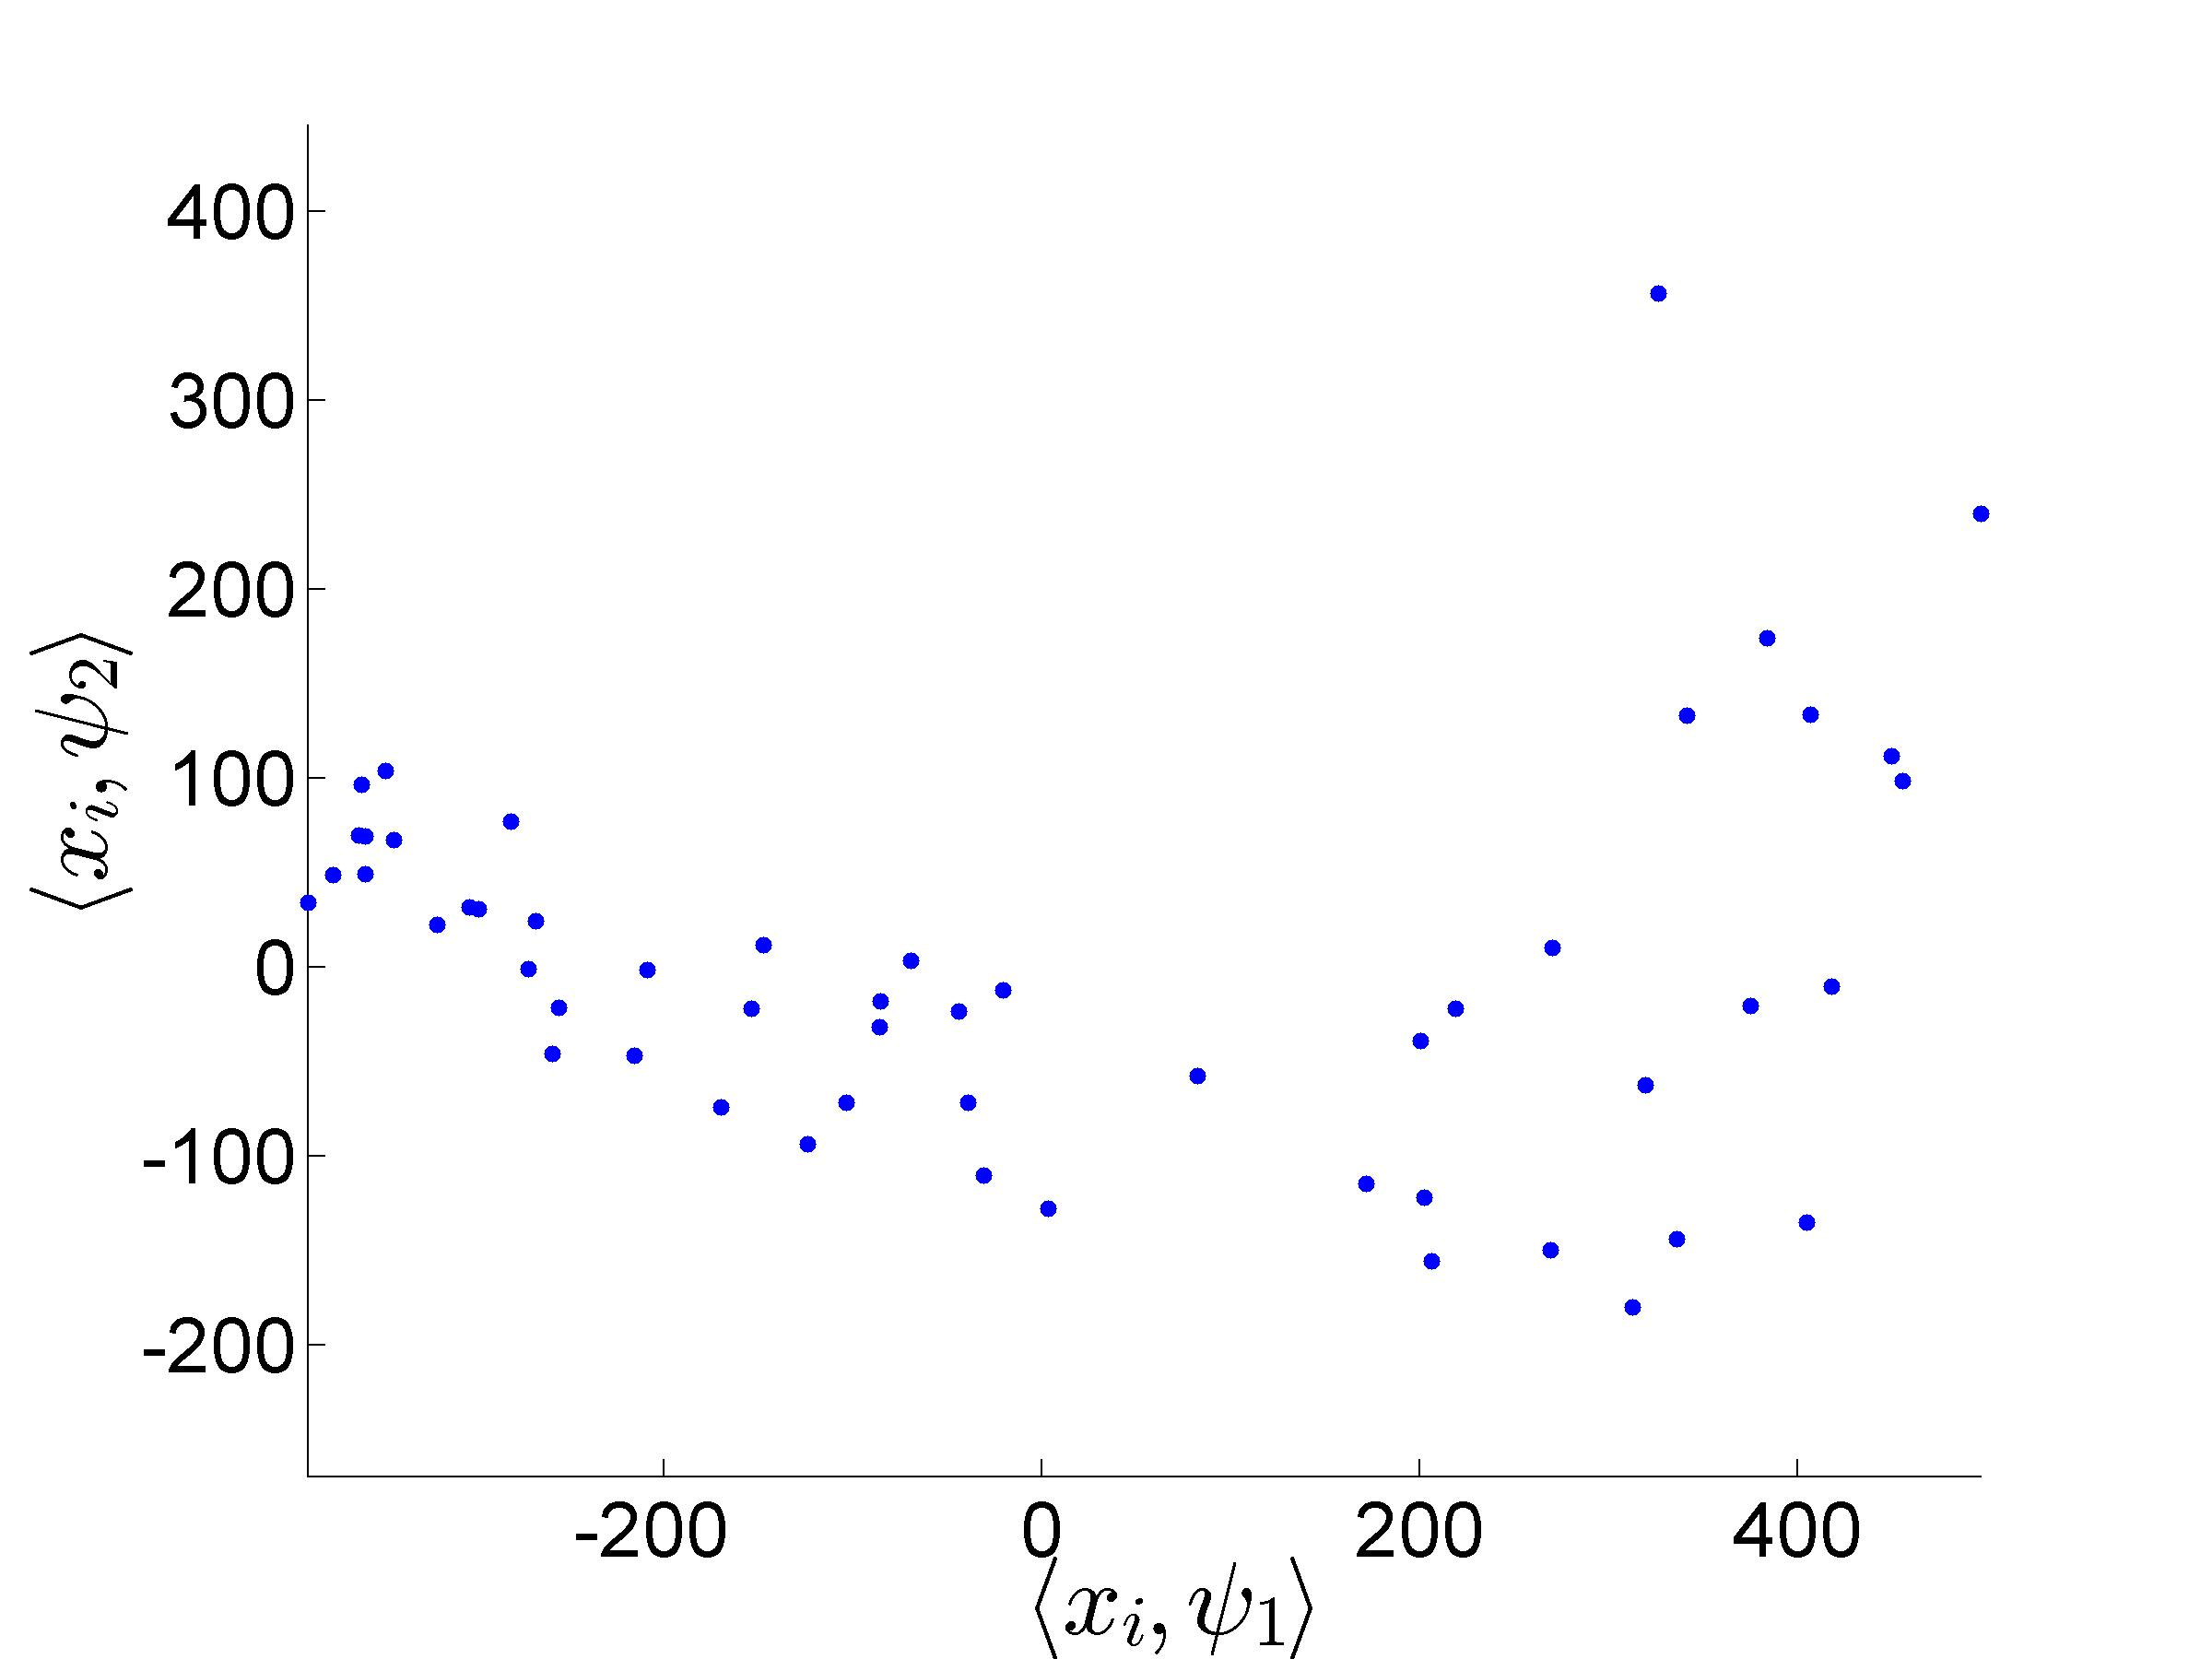
\includegraphics[width=\textwidth]{coeff_12_new}
\caption{}
\label{subfig:PCA_12}
\end{subfigure}
\begin{subfigure}{0.3\textwidth}
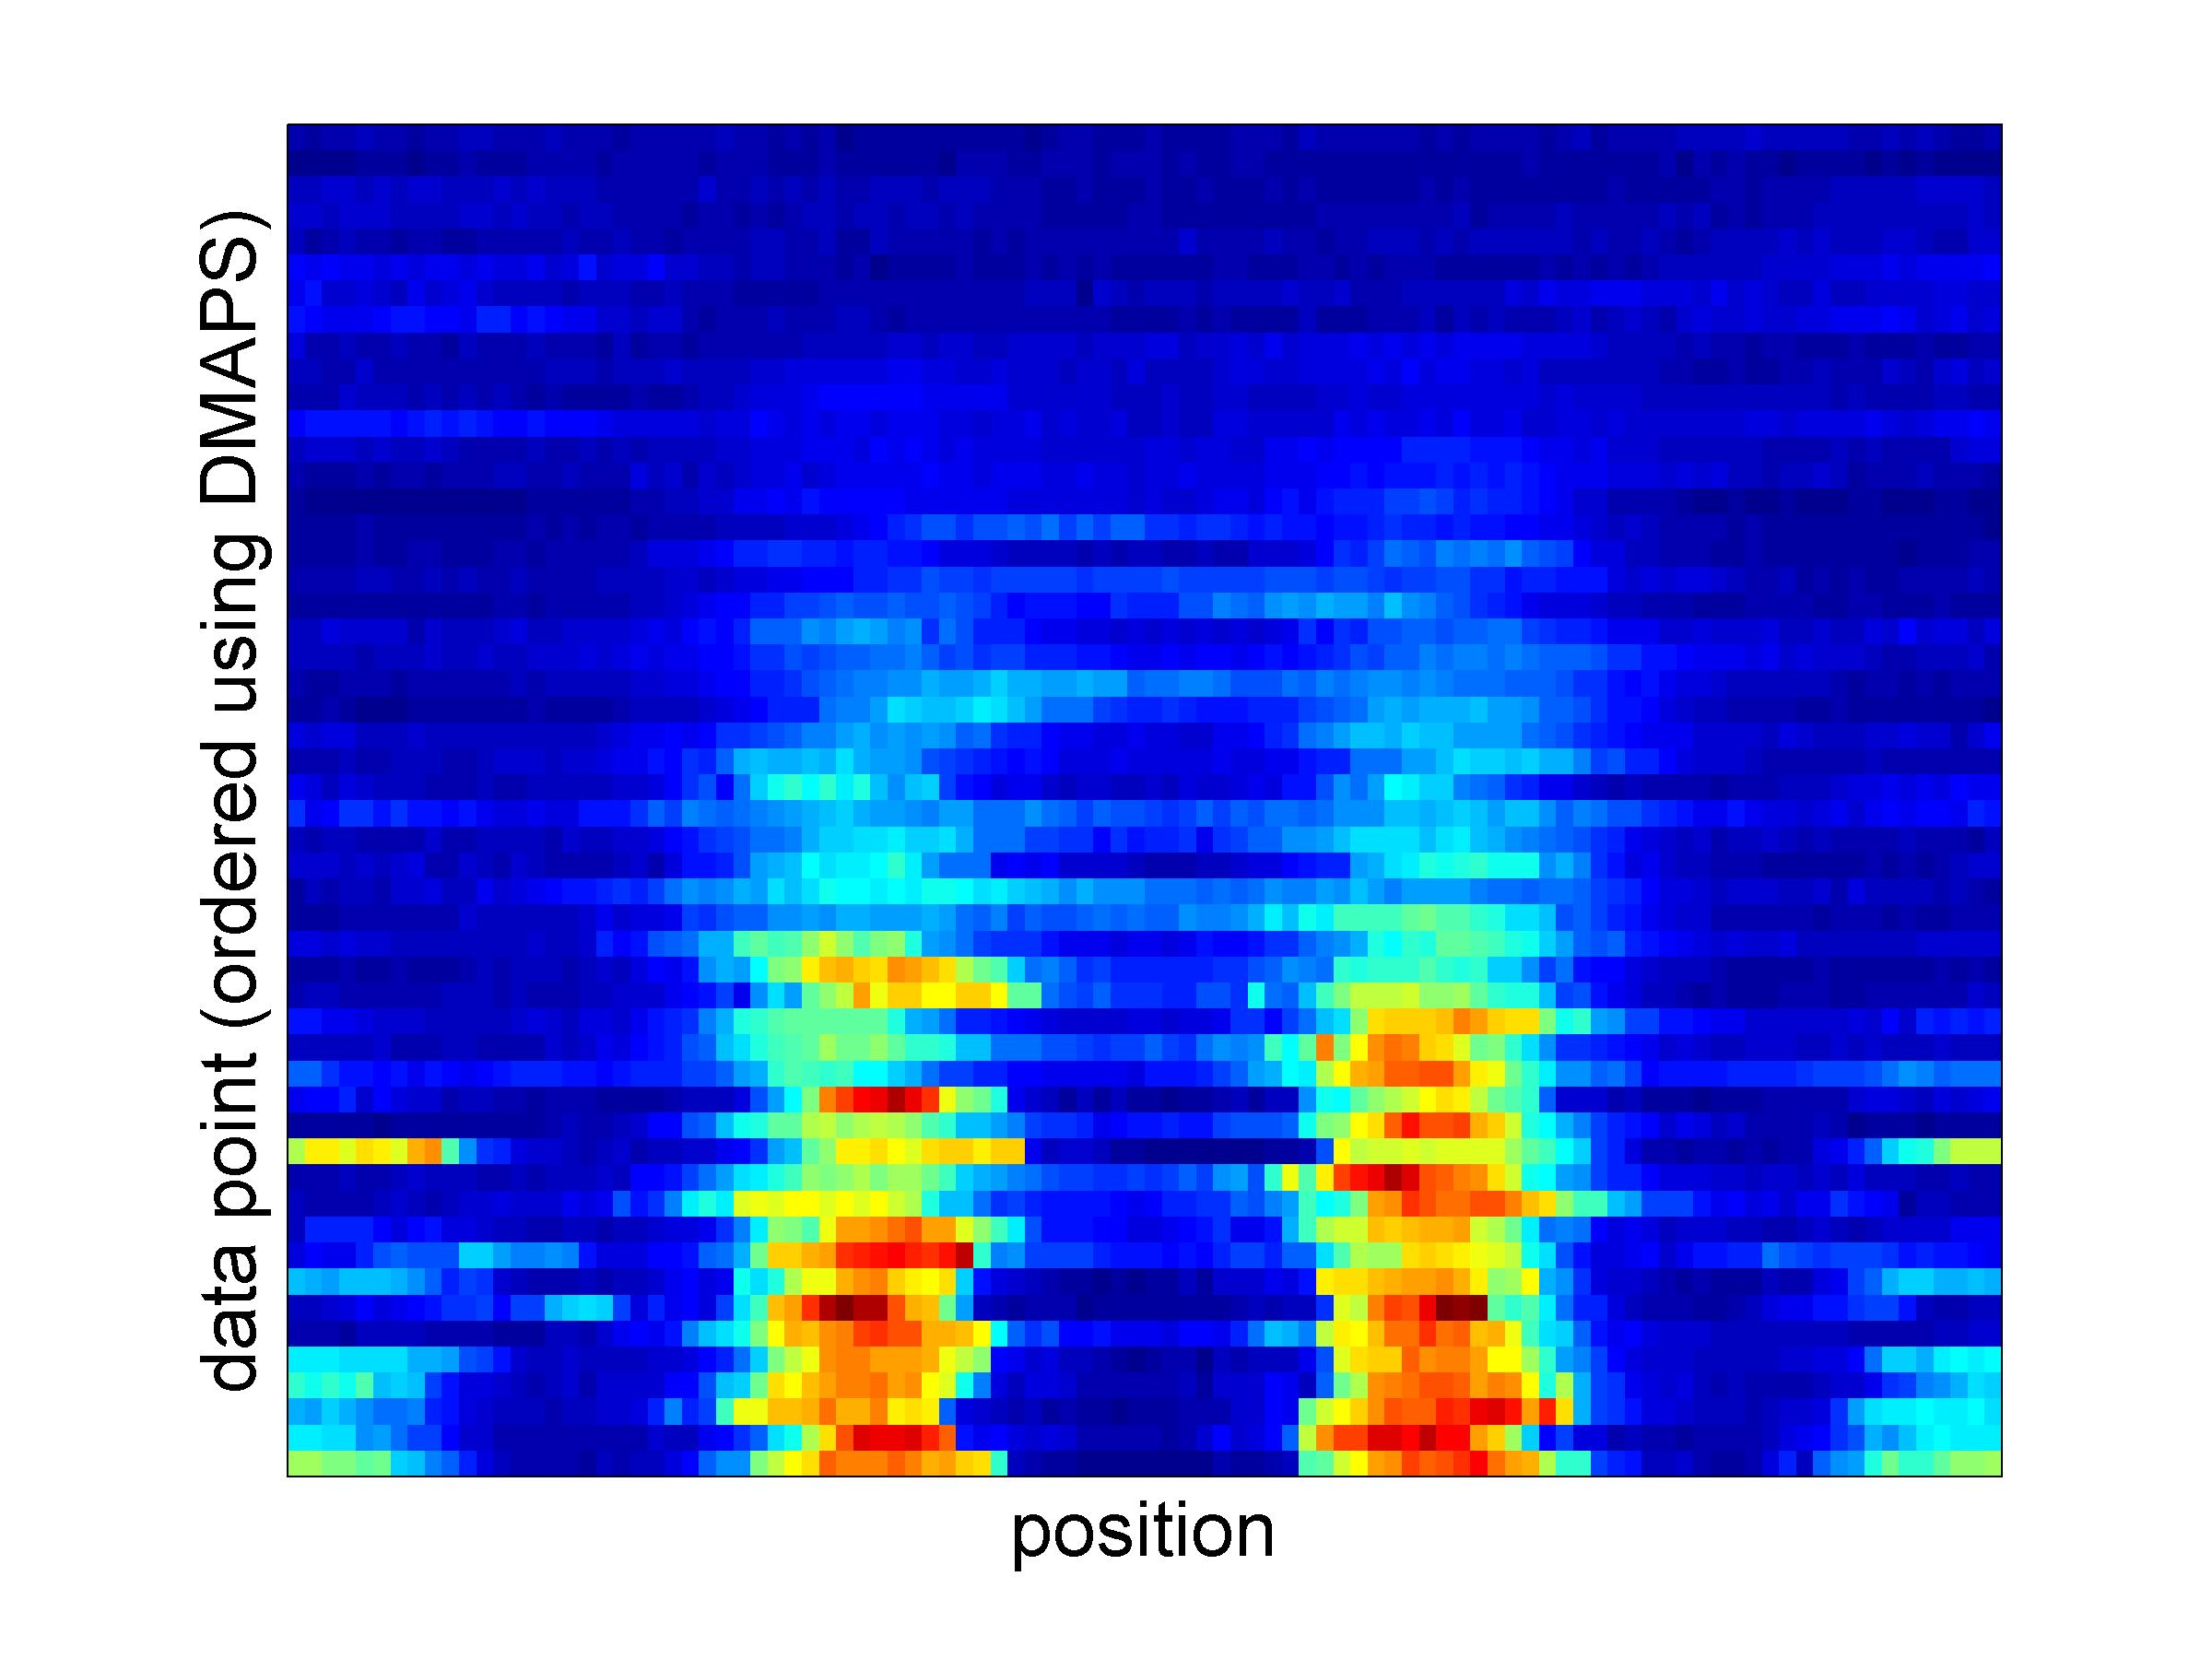
\includegraphics[width=\textwidth]{data_ordered_DMAPS}
\caption{}
\end{subfigure}
\begin{subfigure}{0.3\textwidth}
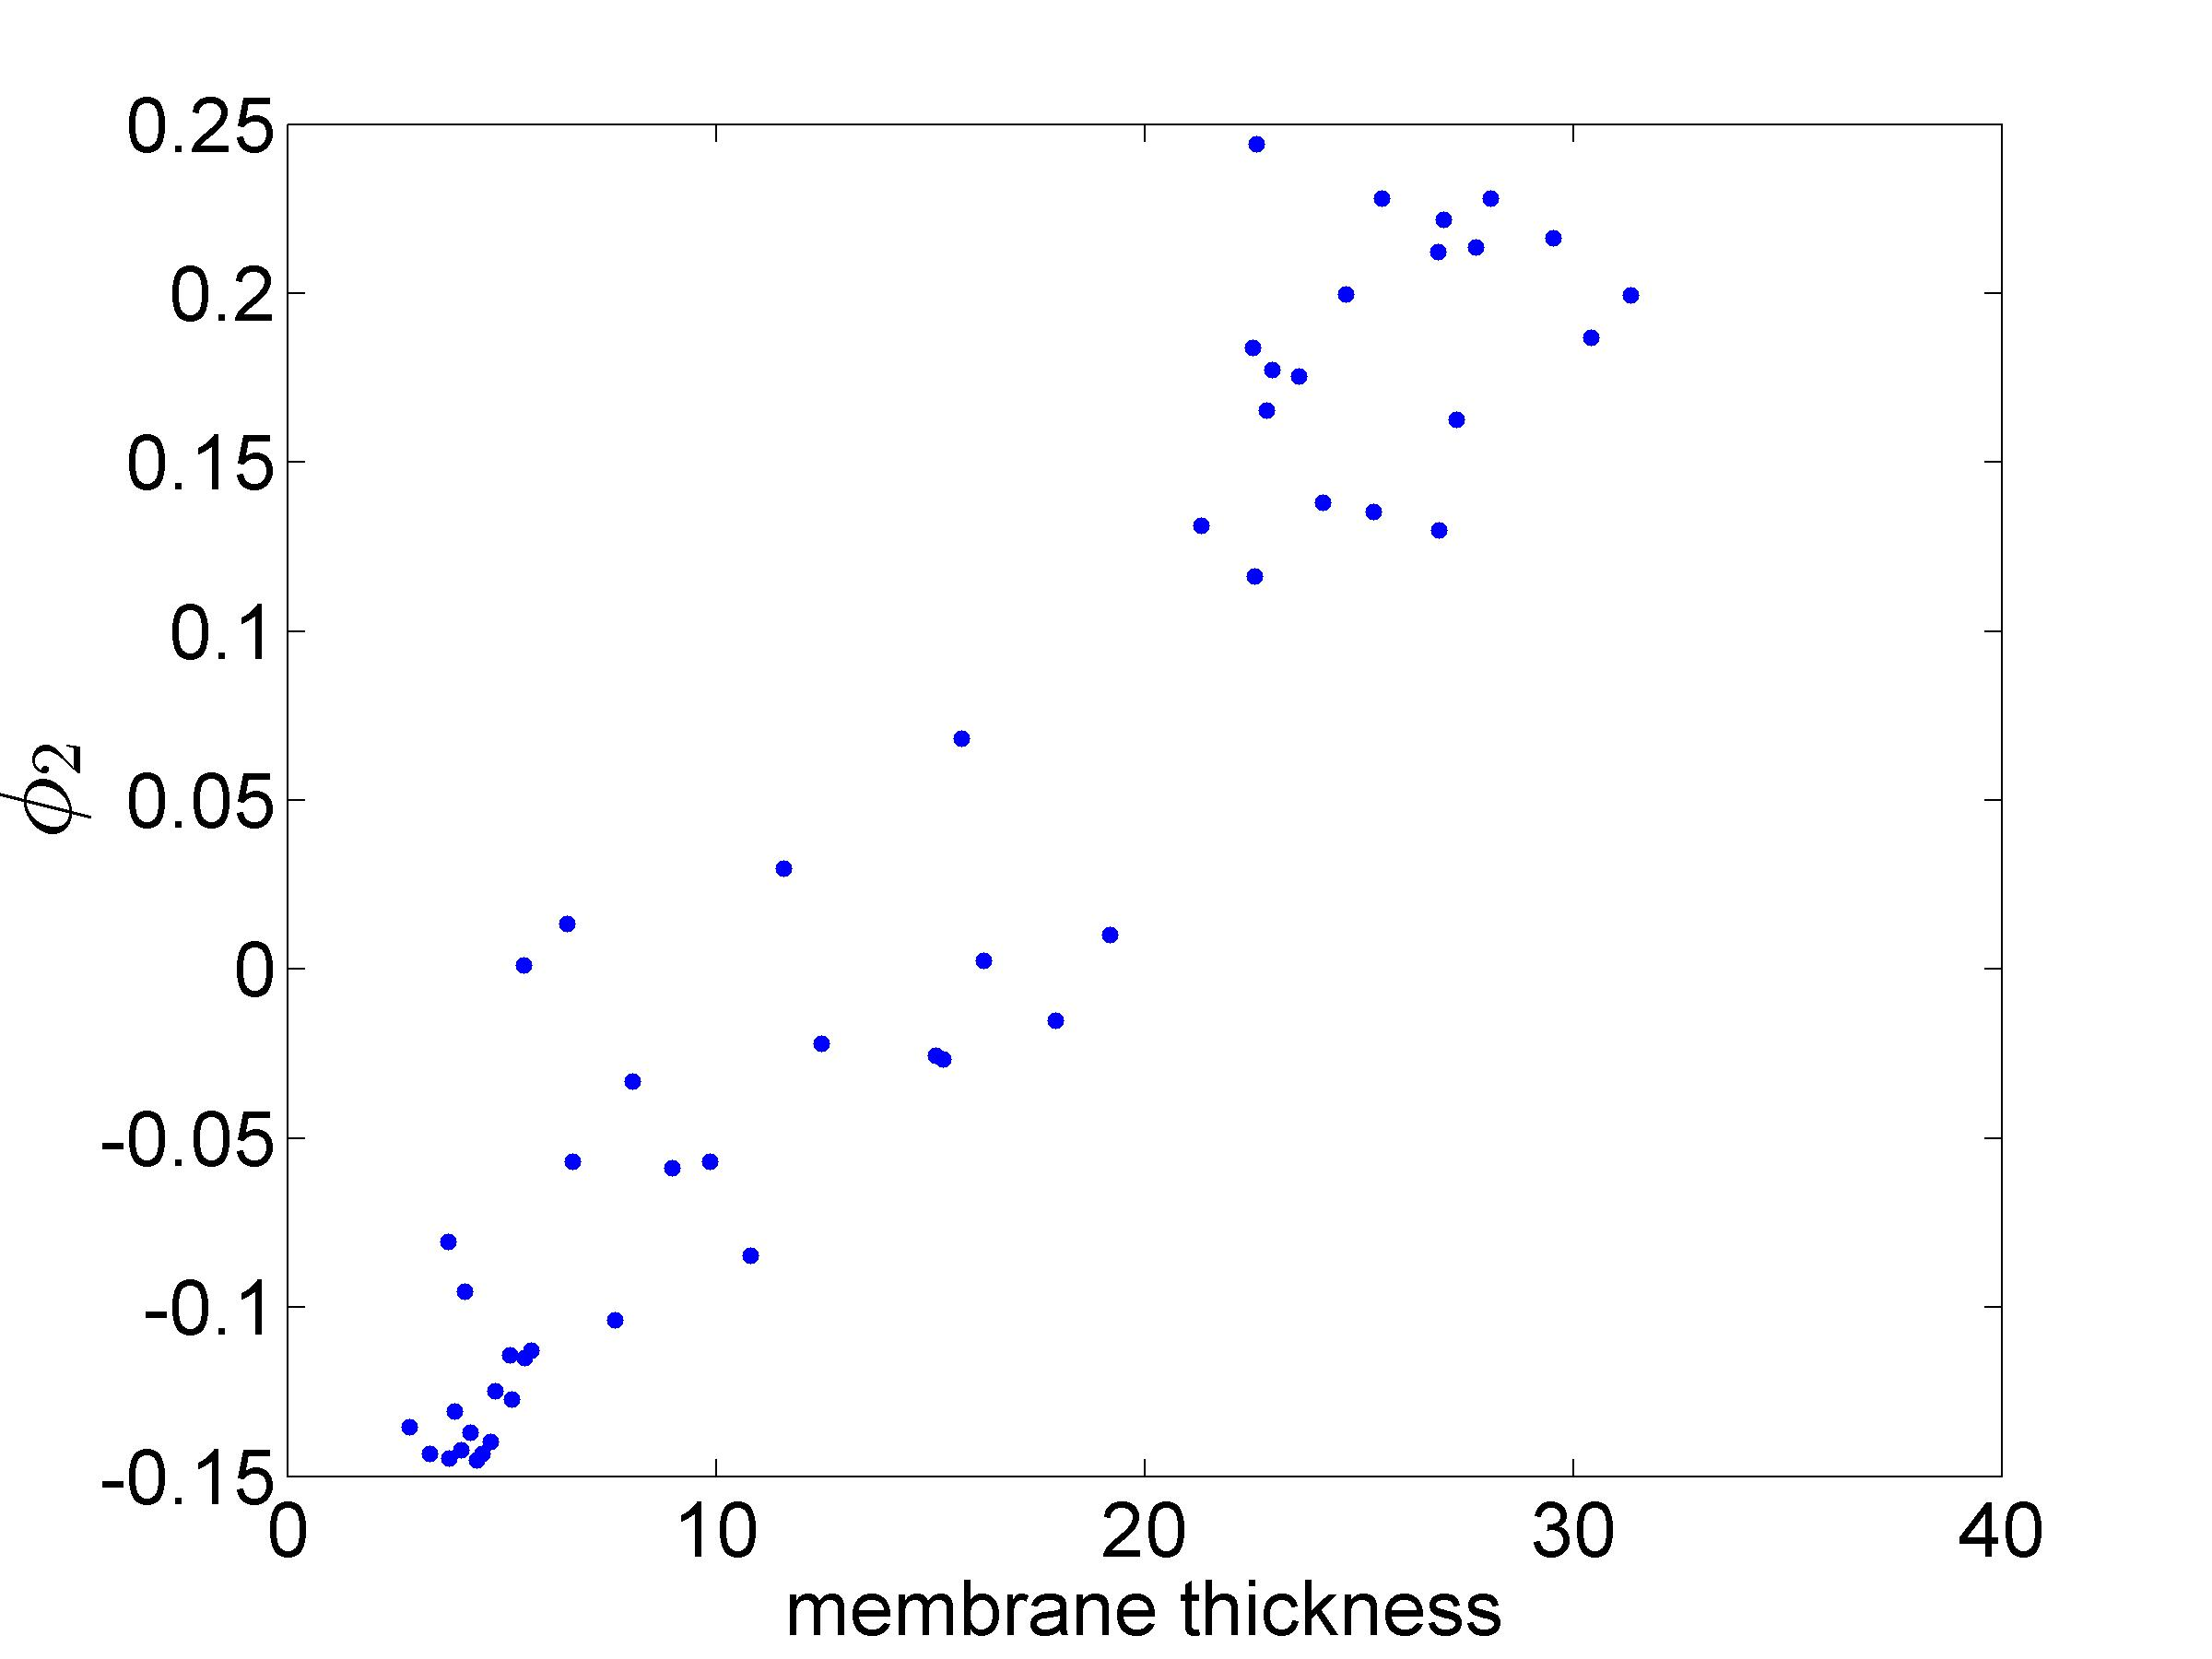
\includegraphics[width=\textwidth]{DMAPS_time_corr}
\caption{}
\end{subfigure}
\caption{{\bf Ordering dpERK concentration profiles using DMAPS.} (a) Projection of data shown in Figure \ref{subfig:unordered_profiles} onto the first two principal components; note that the data falls on an (effectively) one-dimensional, nonlinear curve. 
(b) Concentration profiles of dpERK from (a), now ordered by the first non-trivial DMAPS embedding coordinate.
(c) Correlation between the first (non-trivial) DMAPS embedding coordinate and the membrane thickness.}
\label{fig:DMAPS_ordering}
\end{figure}

\subsection*{dpERK concentration profiles aligned using angular synchronization}

As we have shown, we can order the concentration profiles using PCA or DMAPS.
%
However, ordering the profiles first requires that we factor out the relevant symmetries in the problem.
%
The developmental dynamics are invariant to the oritentation of the embryo in the microfluidic device; therefore, to obtain meaningful results from our analysis, we must first align the embryo snapshots.
%
Rotation of the embryo cross-sections correspond to translation (with periodic boundary conditions) of the linear profiles we have been considering.
%
In the previous analyses, we have assumed that the profiles have been prealigned using the location of the dorsal protein peak.
%
However, without some {\em a priori} knowledge of the system (i.e. knowing that dorsal is expressed at one position along the perimeter of the embryo), we would need to align the concentration profiles before doing our analysis.

The most common and perhaps intuitive techniques for alignment are template-based methods \cite{ahuja2007template}, where one chooses are representative data point or shape as a ``template'', and then shifts or rotates each data point to be optimally aligned with this template.
%
Although these methods are simple, they require knowledge of an appropriate template function and can suffer when the data set is noisy.
%
Angular synchronization \cite{singer2011angular} is a relatively new technique that is often more robust than template-based methods in the presence of noise.
%
We used angular synchronization to factor out the shifts in the concentration profiles measured from the fluorescent images.
%
After aligning the data points using angular synchronization, we used DMAPS to order the aligned concentration profiles.
%
The results are shown in Figure \ref{fig:angsynch_ordering}.
%
One can see that the results are visually consistent with the results shown in Figure \ref{fig:DMAPS_ordering}. 

\begin{figure}[H]
\begin{subfigure}{0.3\textwidth}
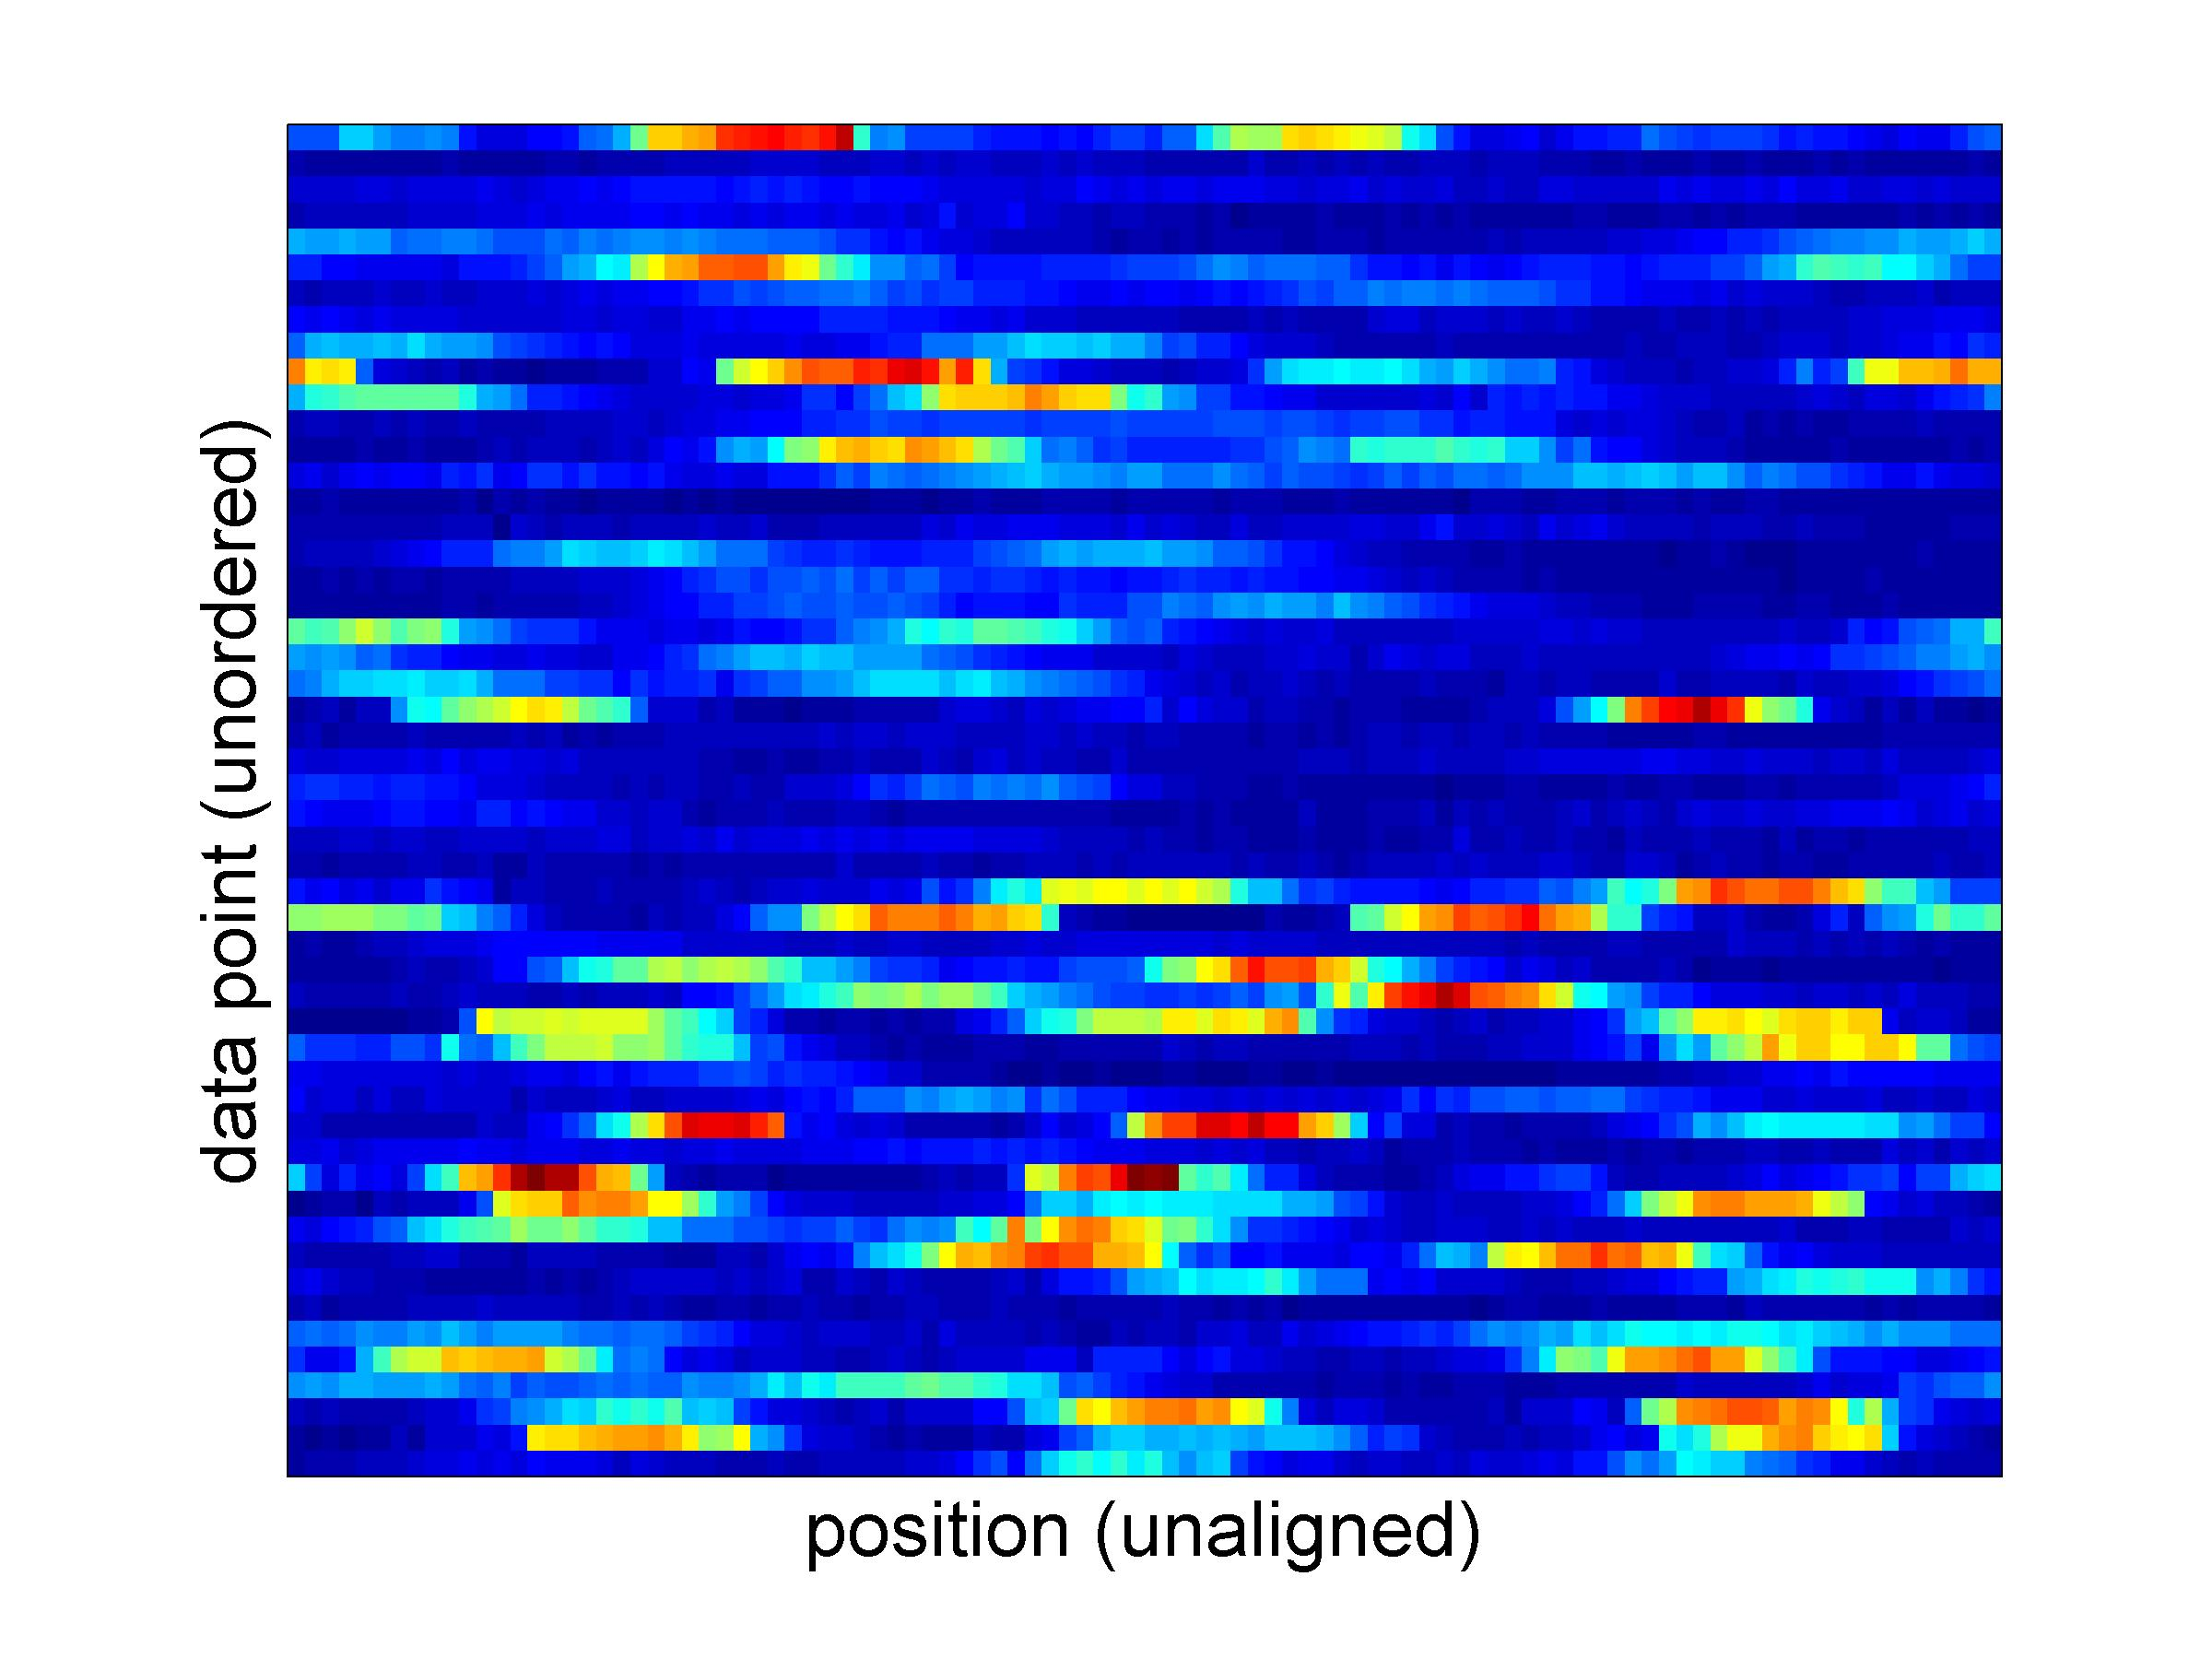
\includegraphics[width=\textwidth]{data_unaligned_unordered}
\caption{}
\end{subfigure}
\begin{subfigure}{0.3\textwidth}
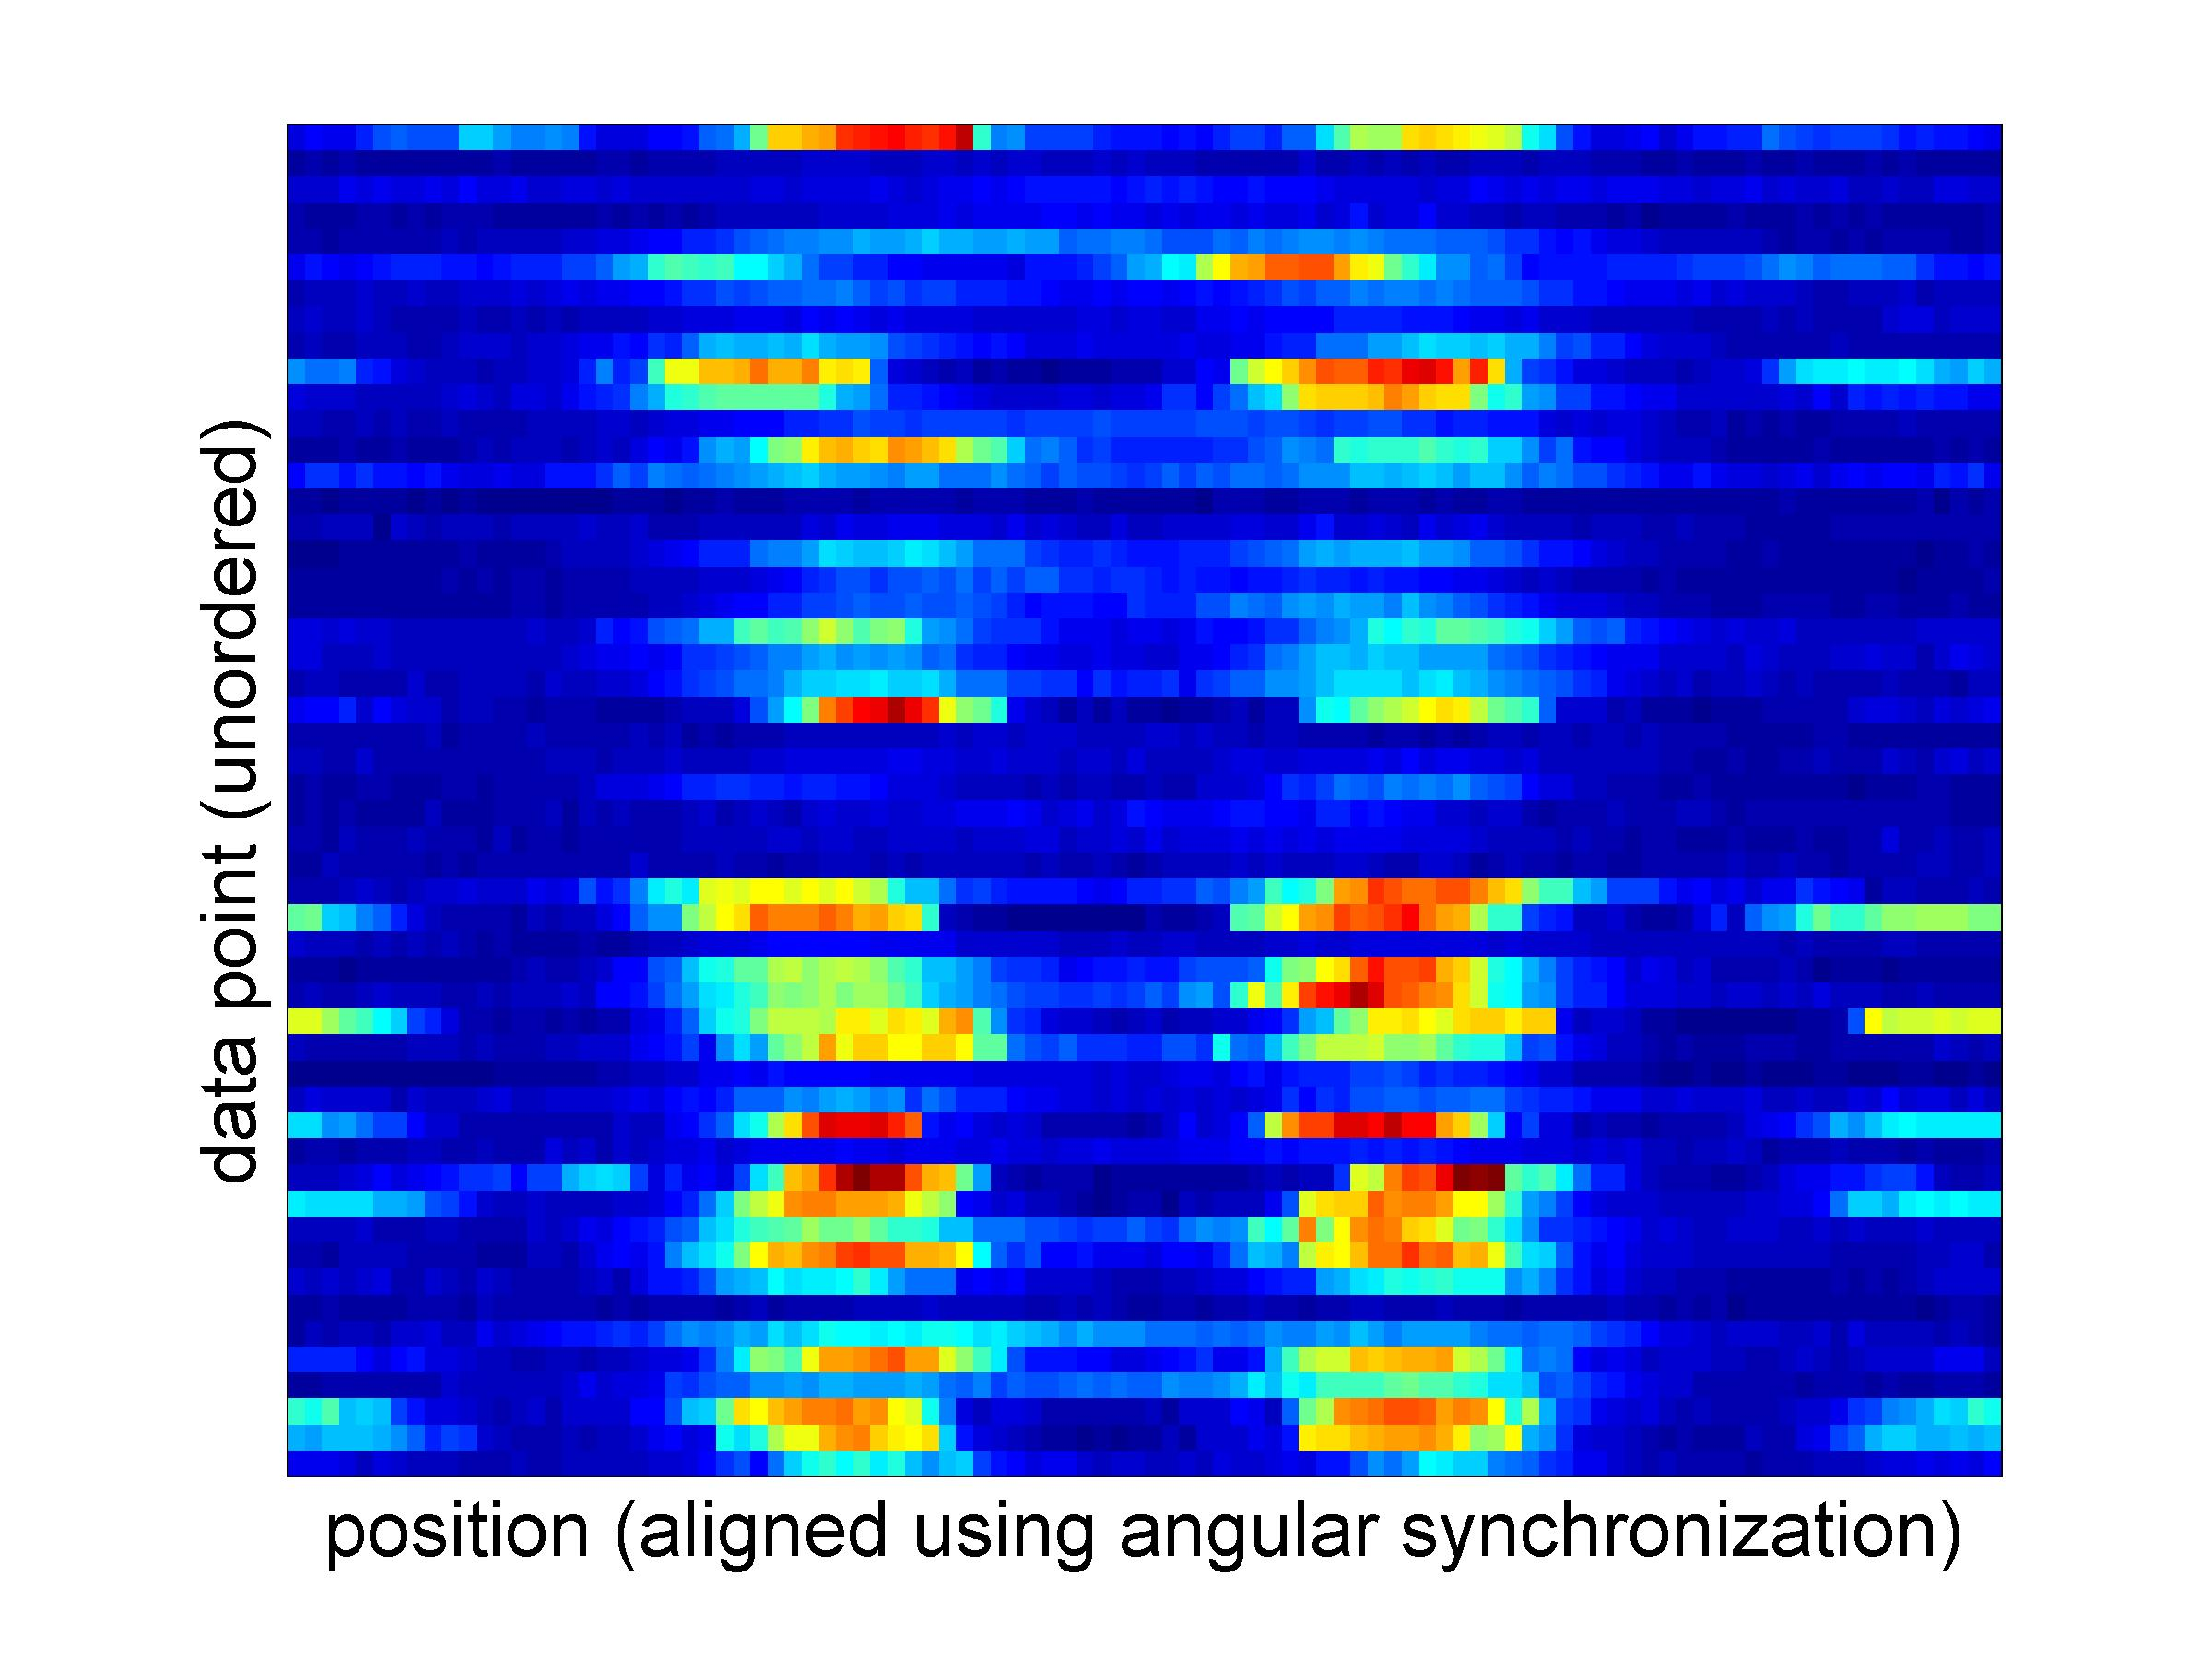
\includegraphics[width=\textwidth]{data_aligned_unordered}
\caption{}
\end{subfigure}
\begin{subfigure}{0.3\textwidth}
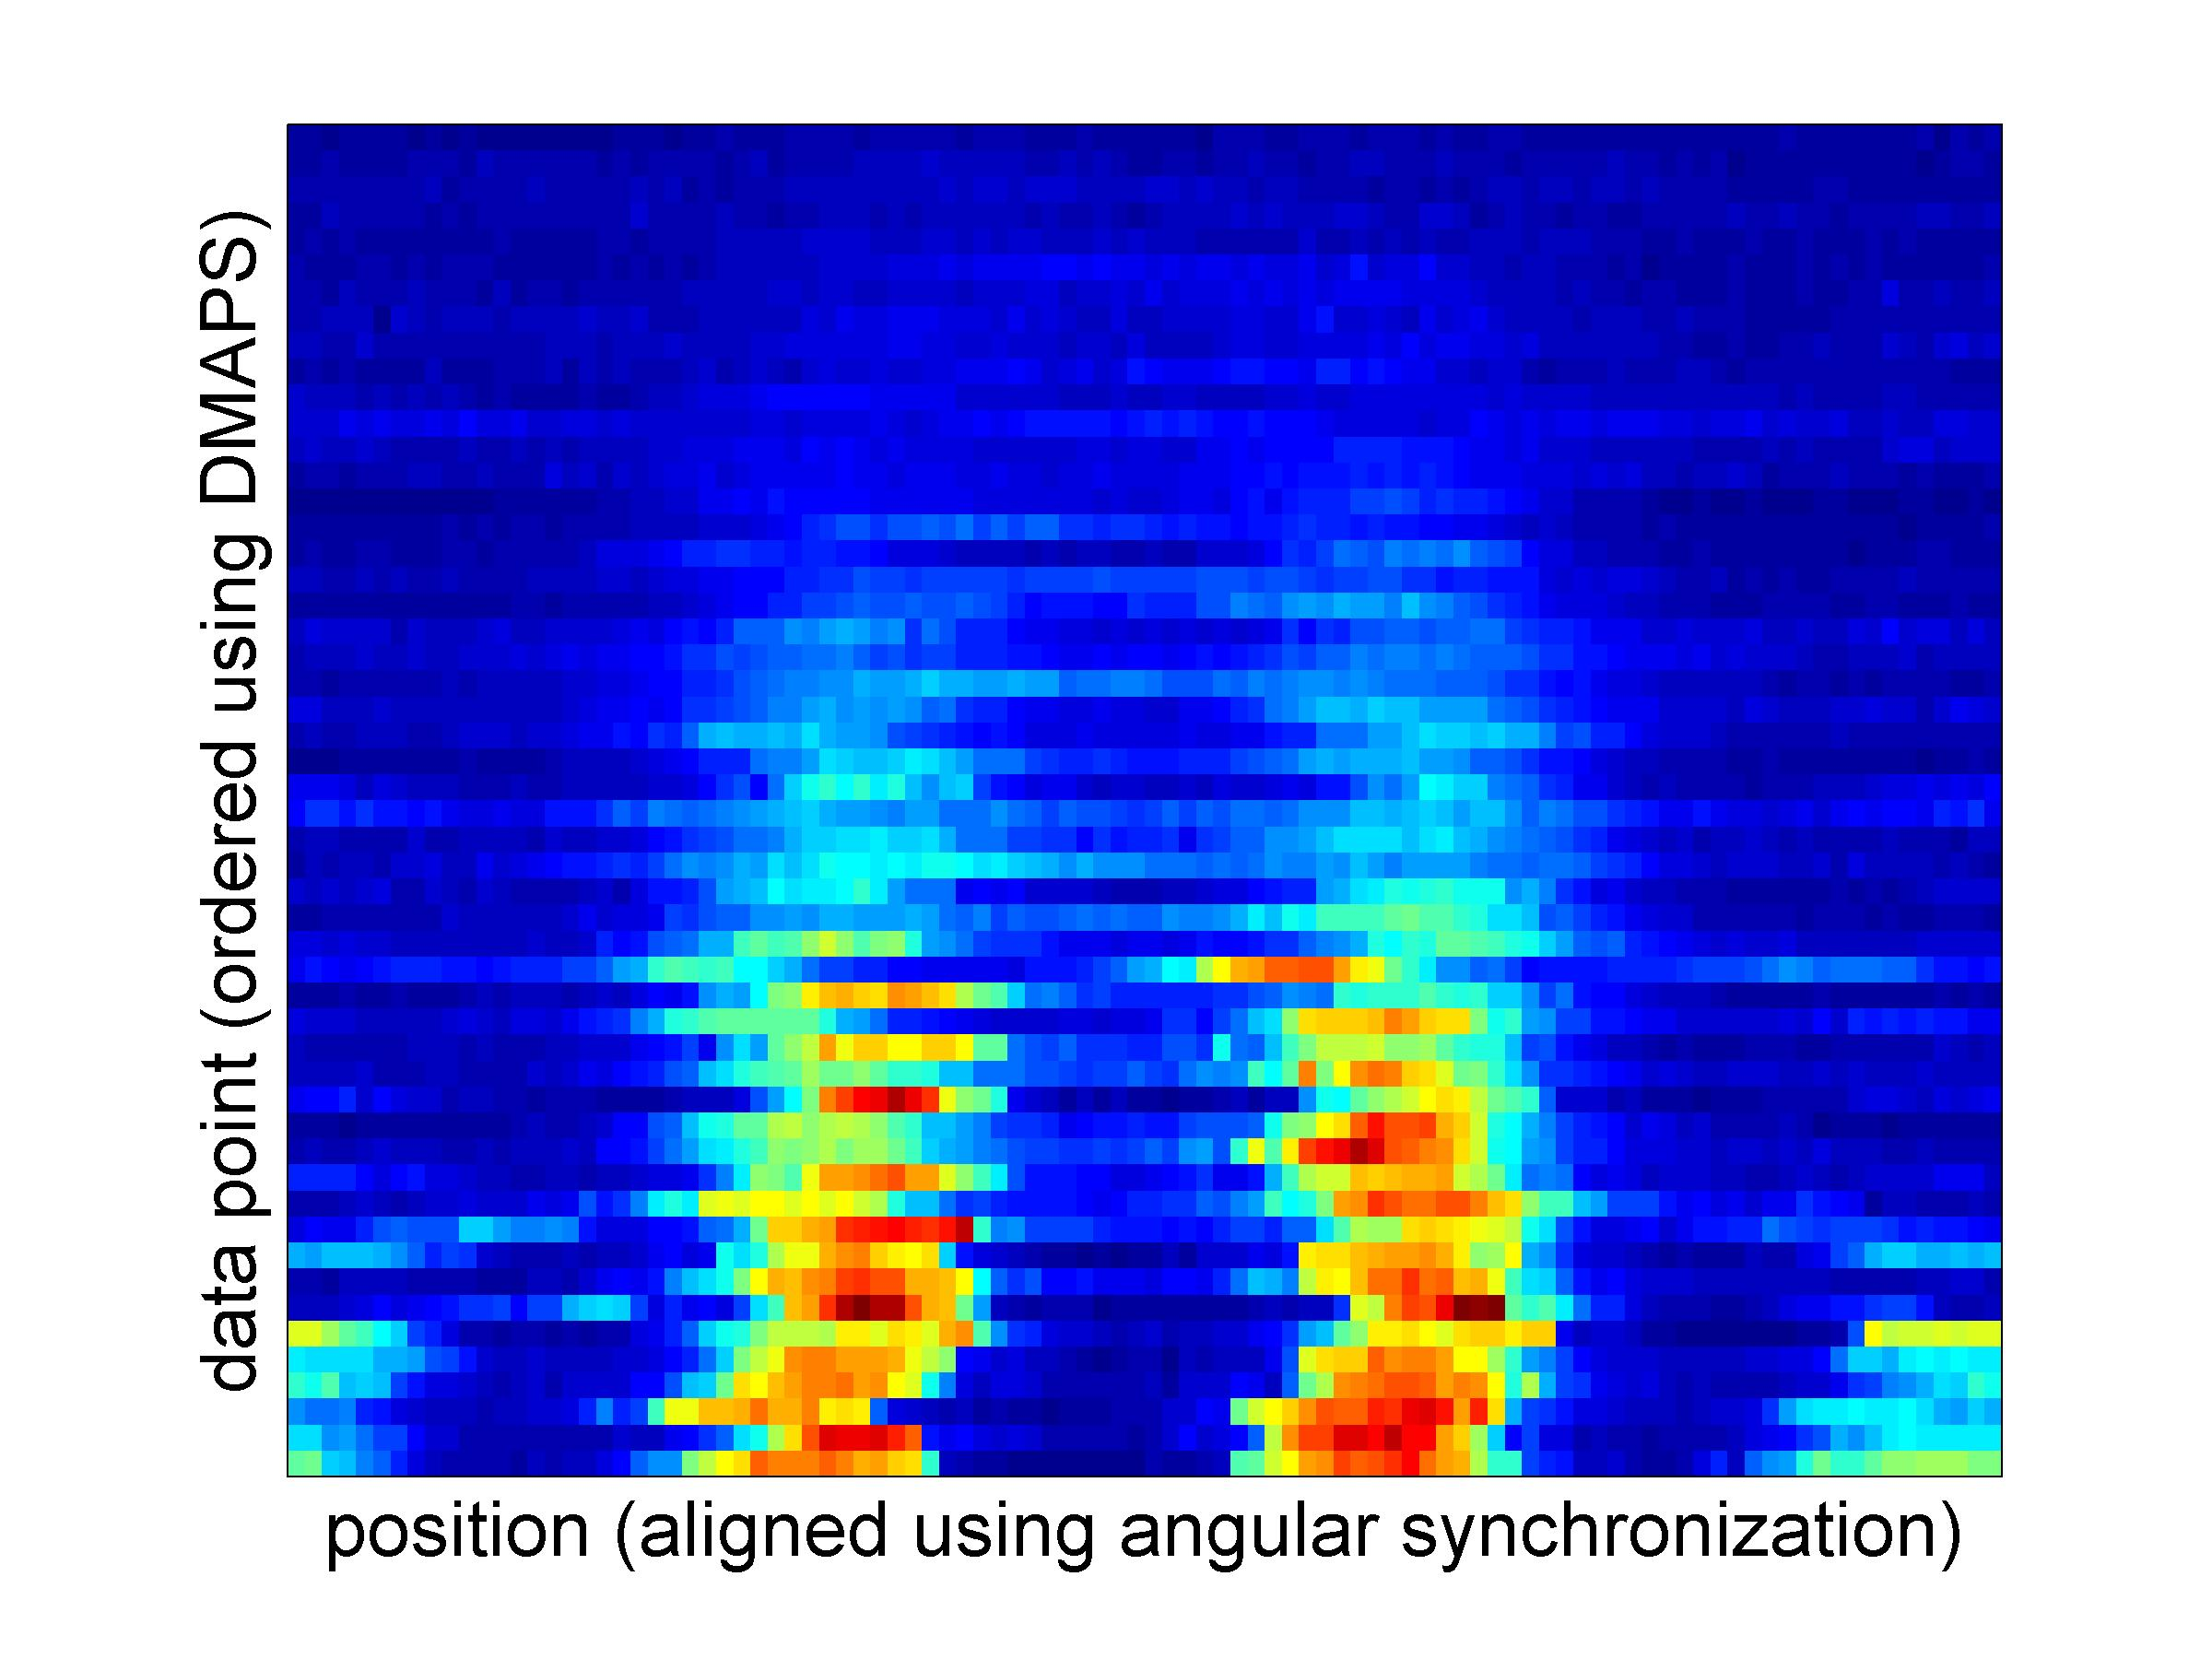
\includegraphics[width=\textwidth]{data_ordered_angsynch}
\caption{}
\end{subfigure}
\caption{{\bf Ordering spatially unaligned dpERK concentration profiles.} (a) Concentration profiles of dpERK for many embryos. Each row represents a different embryo fixed at a slightly different developmental time. The circluar profiles have not been ``opened'' at the same point; rather, each profile was opened at a random point around the embryo. We are allowed to shift the (linear) profiles left and right.
(b) Concentration profiles of dpERK aligned using angular synchronization.
(c) Concentration profiles of dpERK aligned using angular synchronization and ordered by the first (non-trivial) DMAPS embedding coordinate.}
\label{fig:angsynch_ordering}
\end{figure}

\subsection*{dpERK concentration profiles aligned and ordered using vector diffusion maps}

Instead of using angular synchronization and DMAPS, we can do the alignment and dimensionality reduction/ordering in one computation using vector diffusion maps (VDM).
%
VDM is similar to angular synchronization, but it is intended for data sets that contain both underlying symmetries and dynamics.
%
The results of aligning {\em and} ordering the data using VDM are shown in Figure \ref{fig:vdm_ordering}; the results are similar to those from angular syncrhonization (Figure \ref{fig:angsynch_ordering}).

\begin{figure}[H]
\begin{subfigure}{0.3\textwidth}
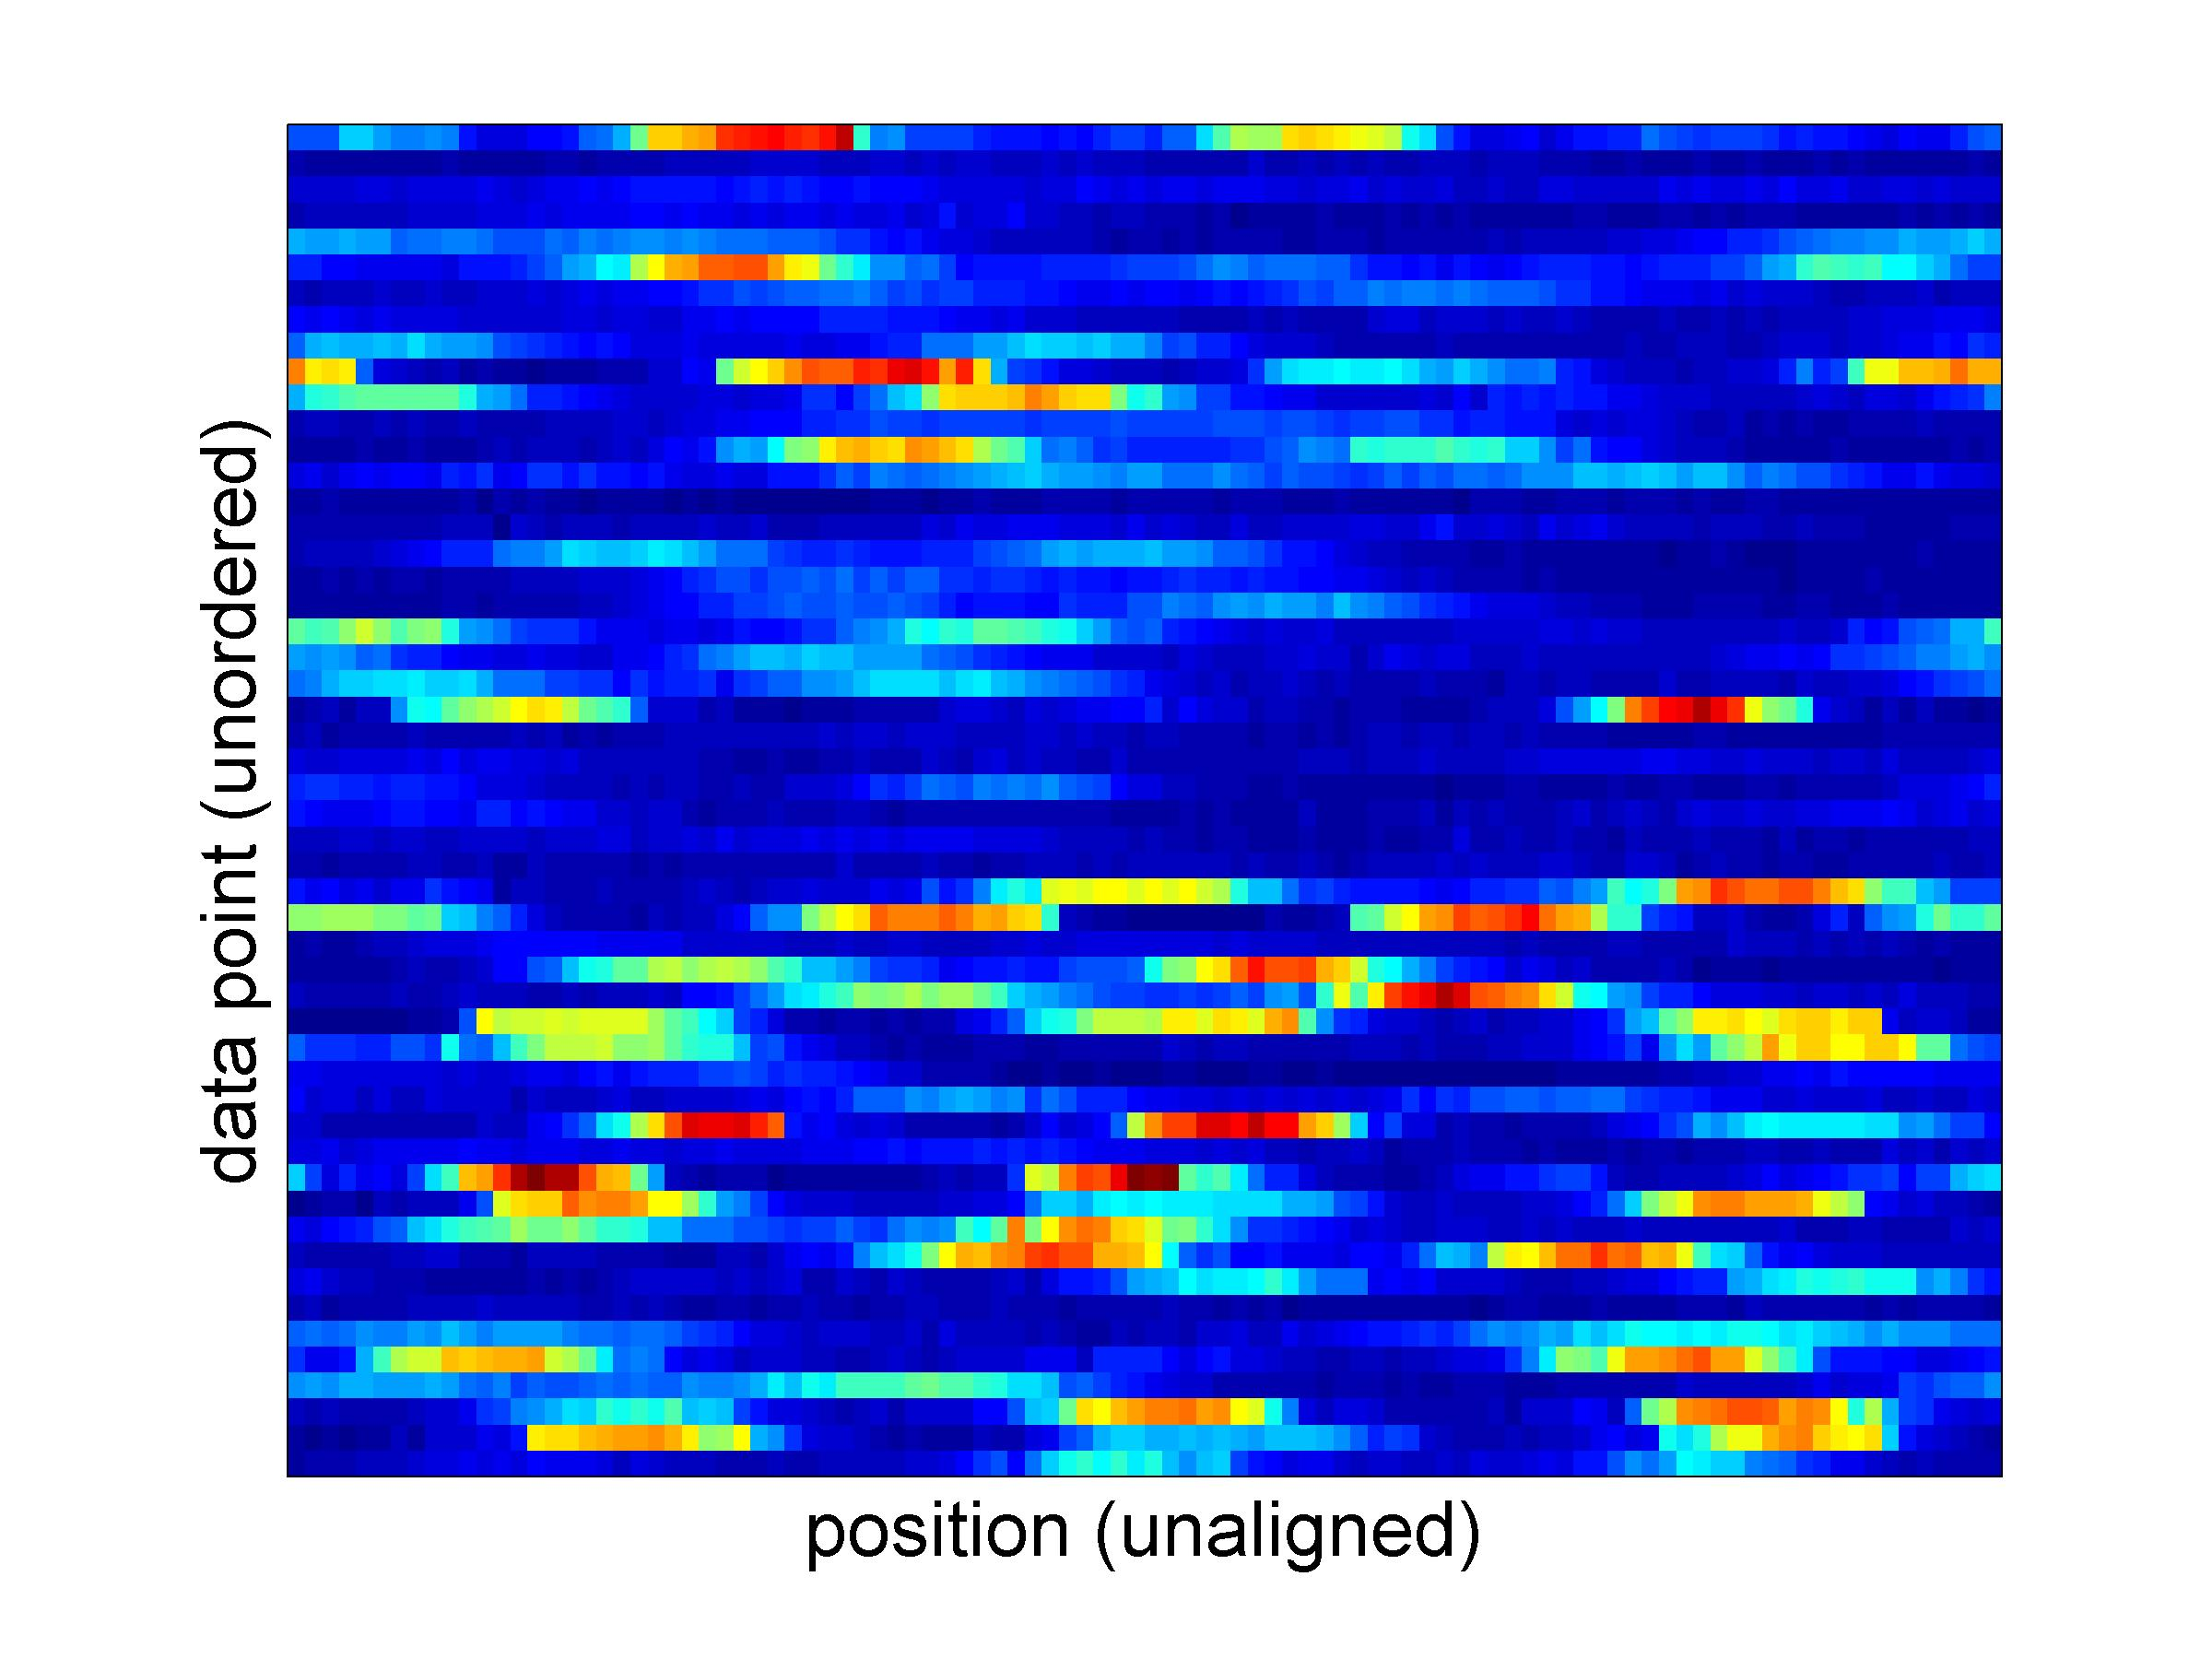
\includegraphics[width=\textwidth]{data_unaligned_unordered}
\caption{}
\end{subfigure}
\begin{subfigure}{0.3\textwidth}
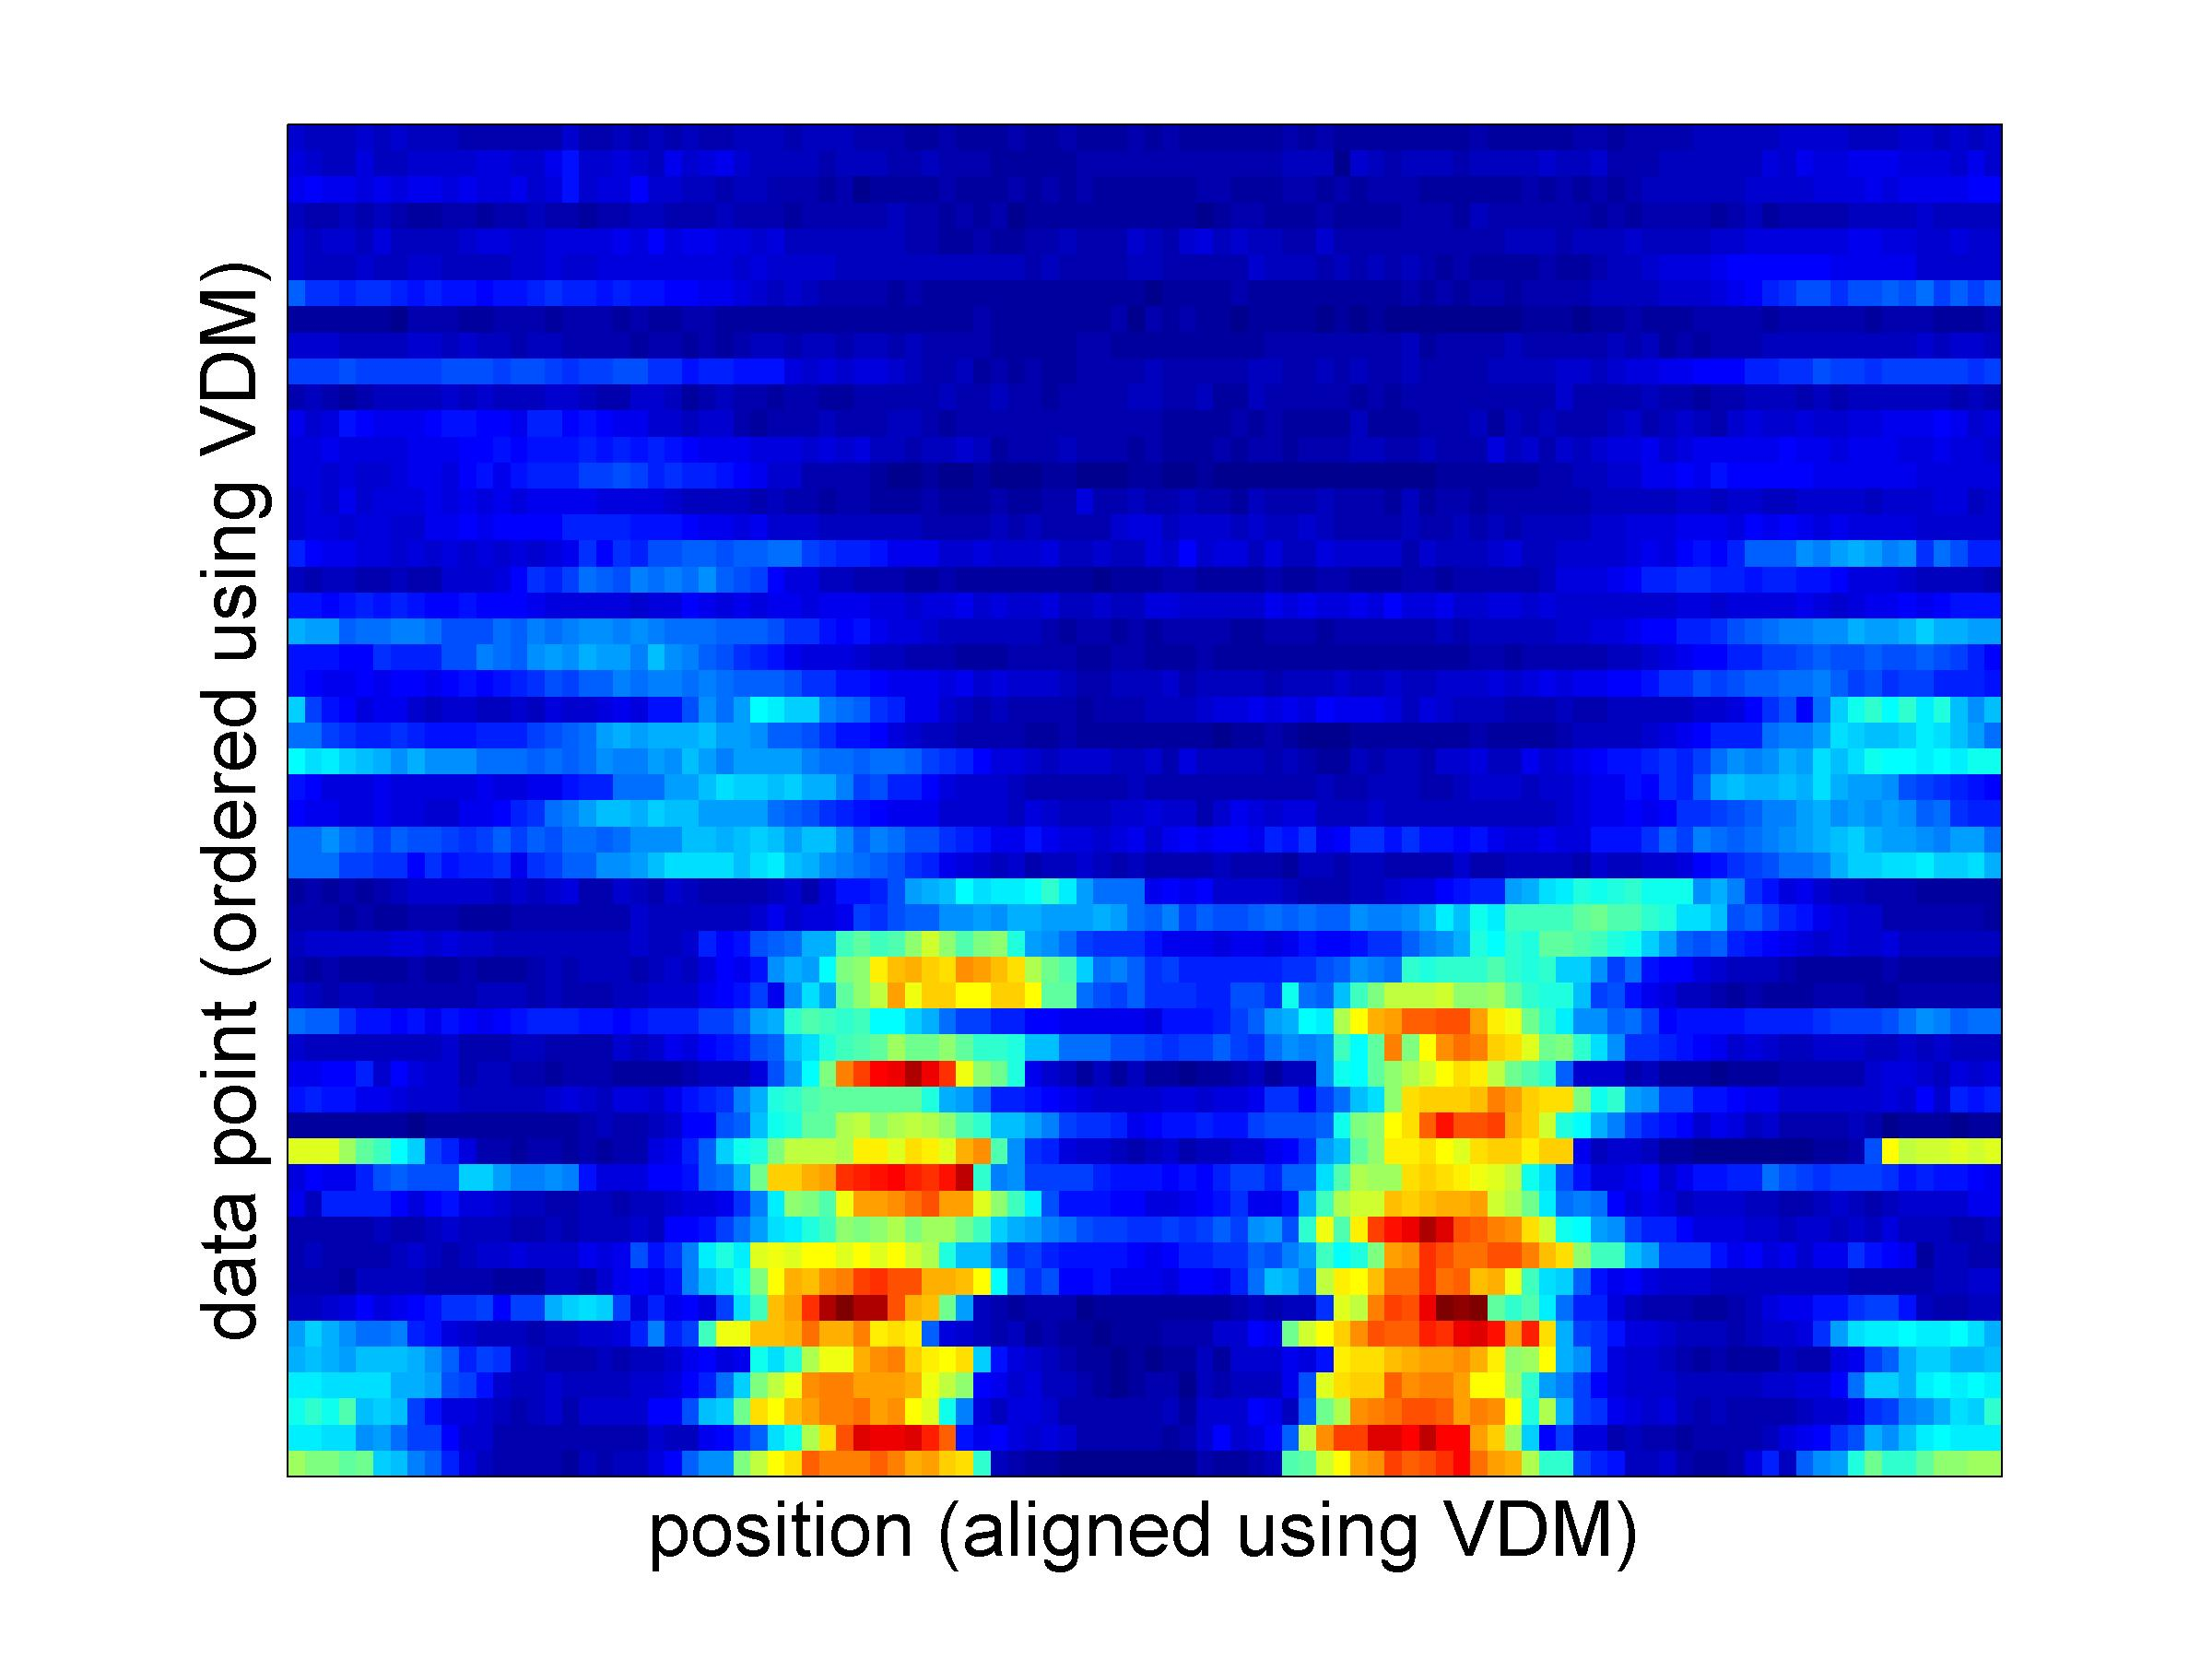
\includegraphics[width=\textwidth]{data_ordered_vdm}
\caption{}
\end{subfigure}
\begin{subfigure}{0.3\textwidth}
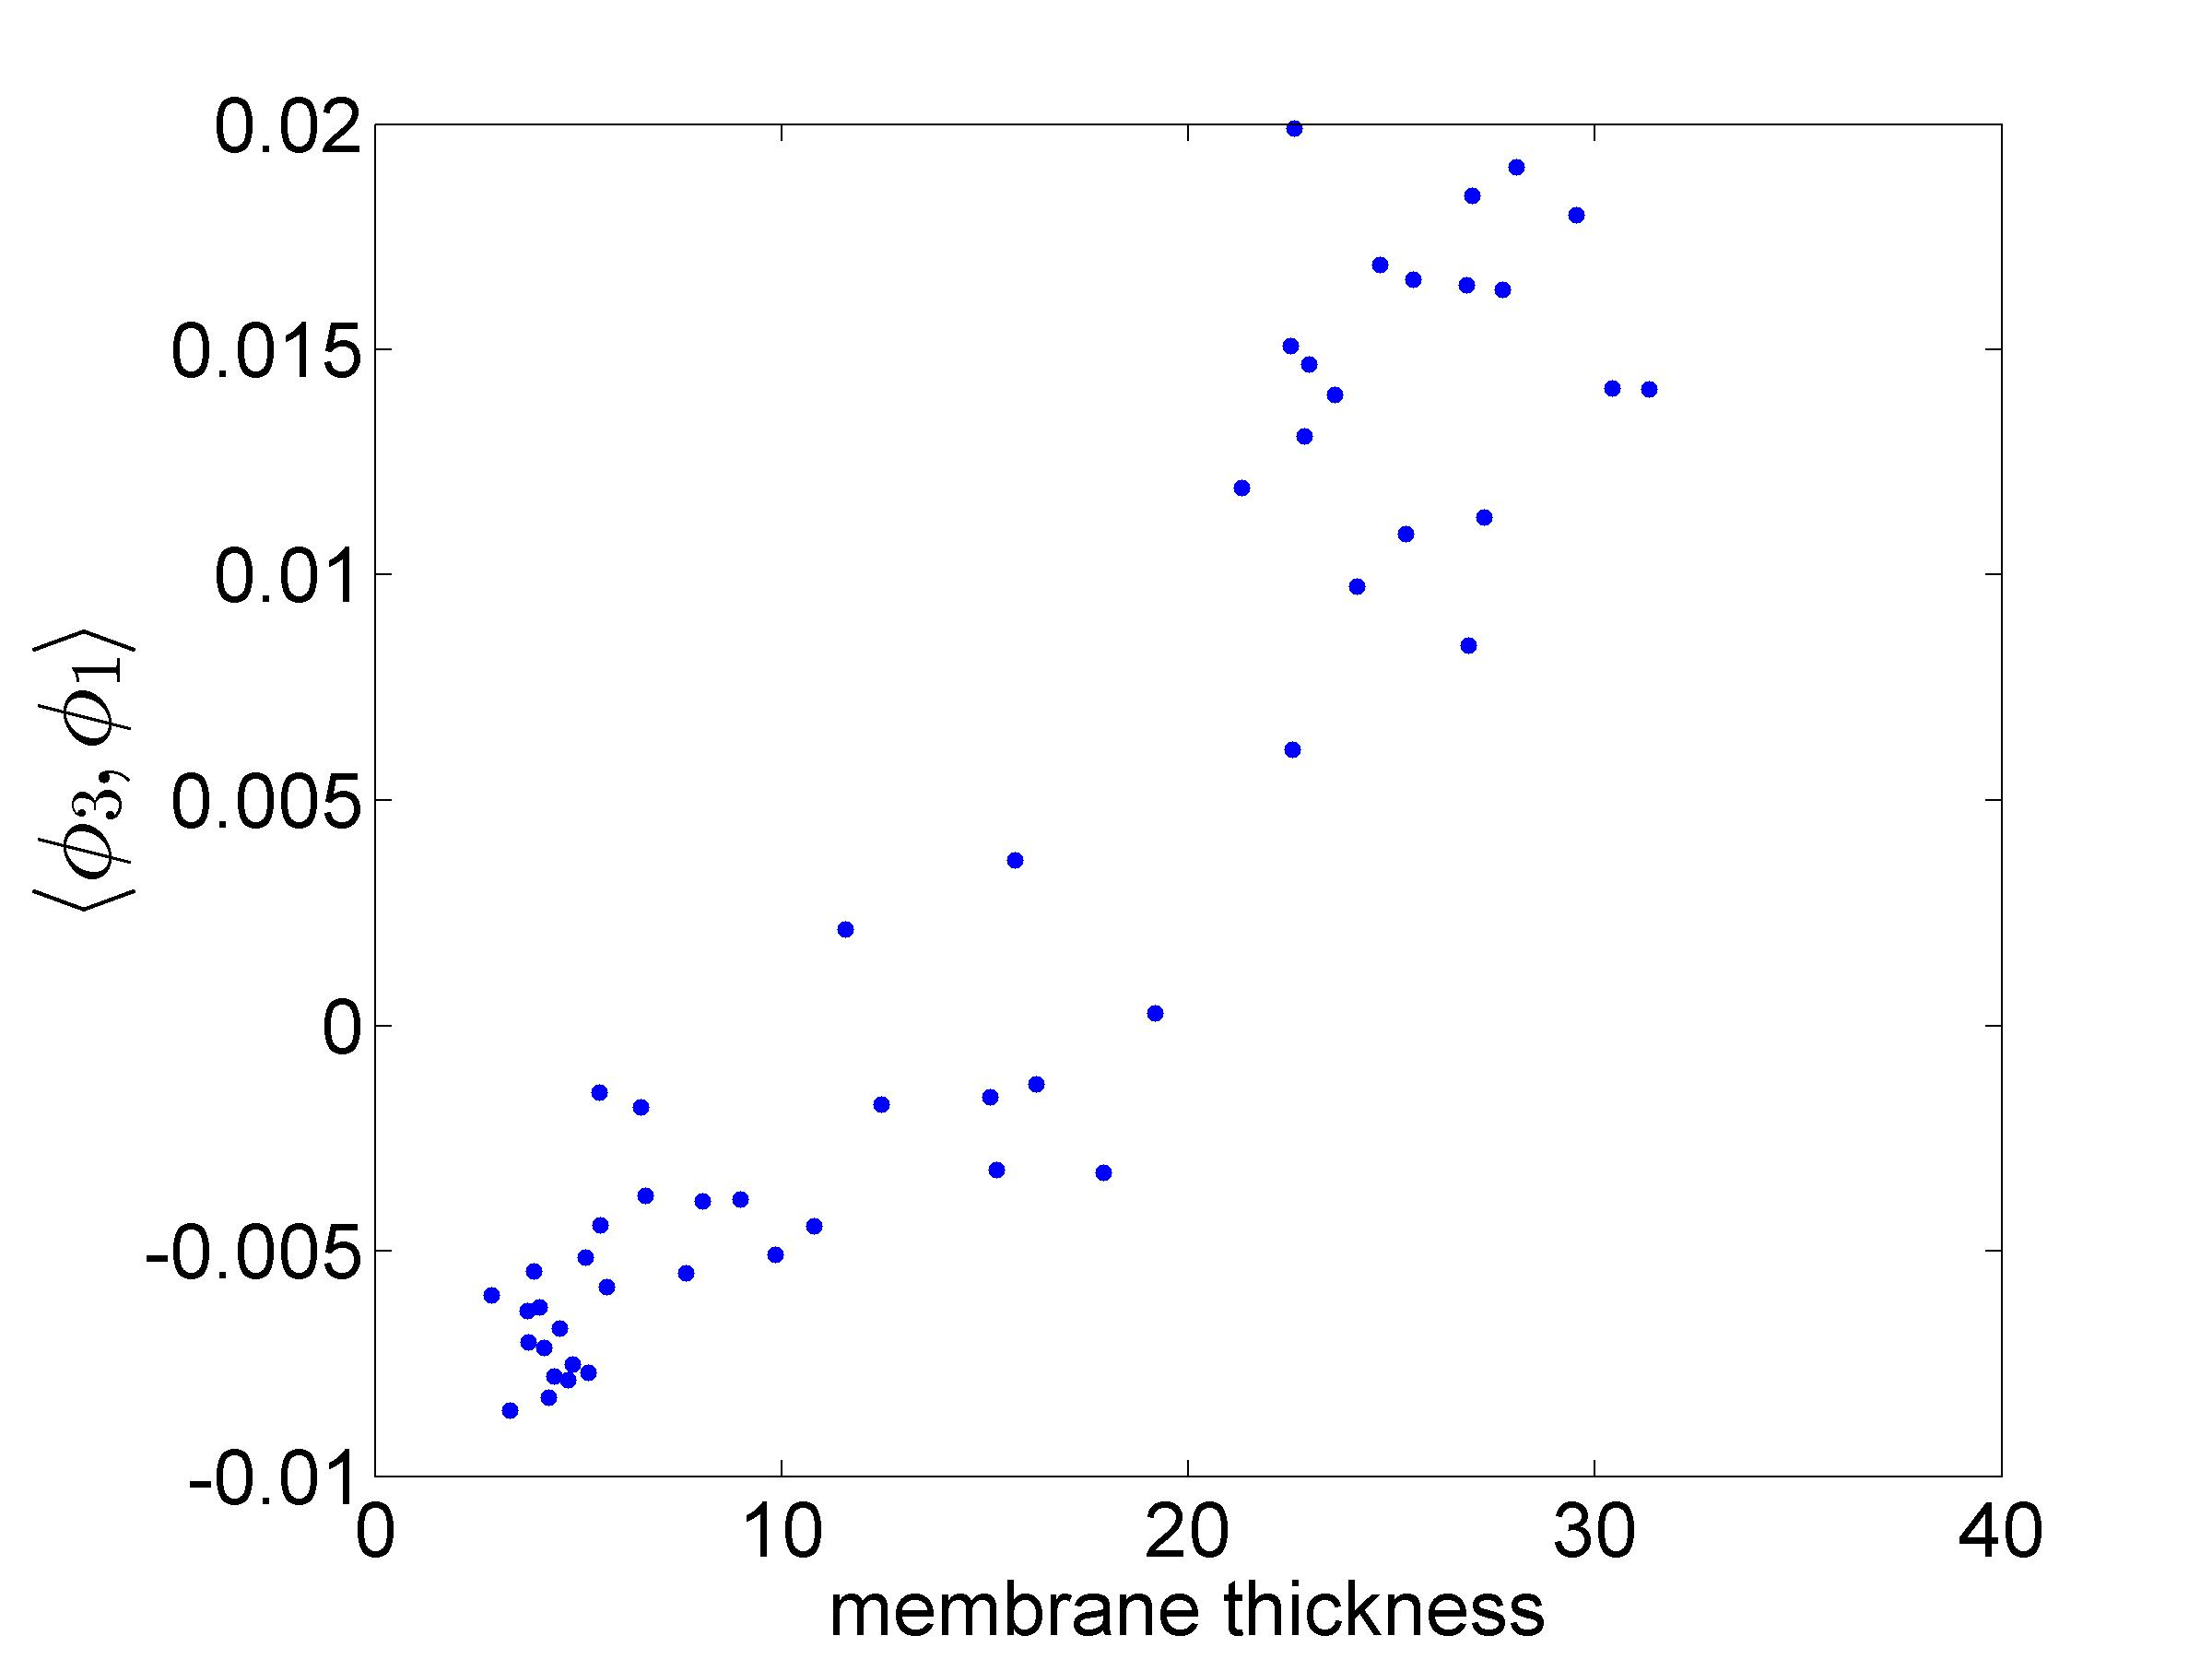
\includegraphics[width=\textwidth]{VDM_time_corr}
\caption{}
\end{subfigure}
\caption{{\bf Ordering spatially unaligned dpERK concentration profiles using vector diffusion maps.} (a) Concentration profiles of dpERK for many embryos. Each row represents a different embryo fixed at a slightly different developmental time. The circluar profiles have not been ``opened'' at the same point; rather, each profile was opened at a random point around the embryo. We are allowed to shift the (linear) profiles left and right.
(b) Concentration profiles of dpERK aligned and ordered using vector diffusion maps.
(c) Correlation between the VDM embedding coordinate and the membrane thickness.}
\label{fig:vdm_ordering}
\end{figure}

\subsection*{Two-dimensional dpERK images aligned and ordered using vector diffusion maps}

Thus far, we have focused on the one-dimensional linear concentration profiles that are extracted from the fluorescent images.
%
However, the techniques we have outlined can also be applied to the two-dimensional fluorescent images. 
%
We use VDM to align and order the fluorescent images stained for dpERK. 
%
We now must factor out translations and rotations in the images. 
%
To do this, we project the images onto a sphere;
rotations and translations of a two-dimensional image then correspond to (three-dimensioanl) rotations of the sphere.
%
We then use VDM to align and order the (projected) images, with the underlying symmetry group $SO(3)$. 
%
The results are shown in Figure \ref{fig:vdm_image_ordering};
the orderings are of comparable quality to those obtained with the one-dimensional profiles, and the dpERK peaks are nicely aligned.

\begin{figure}[H]
\centering
\begin{subfigure}{0.45\textwidth}
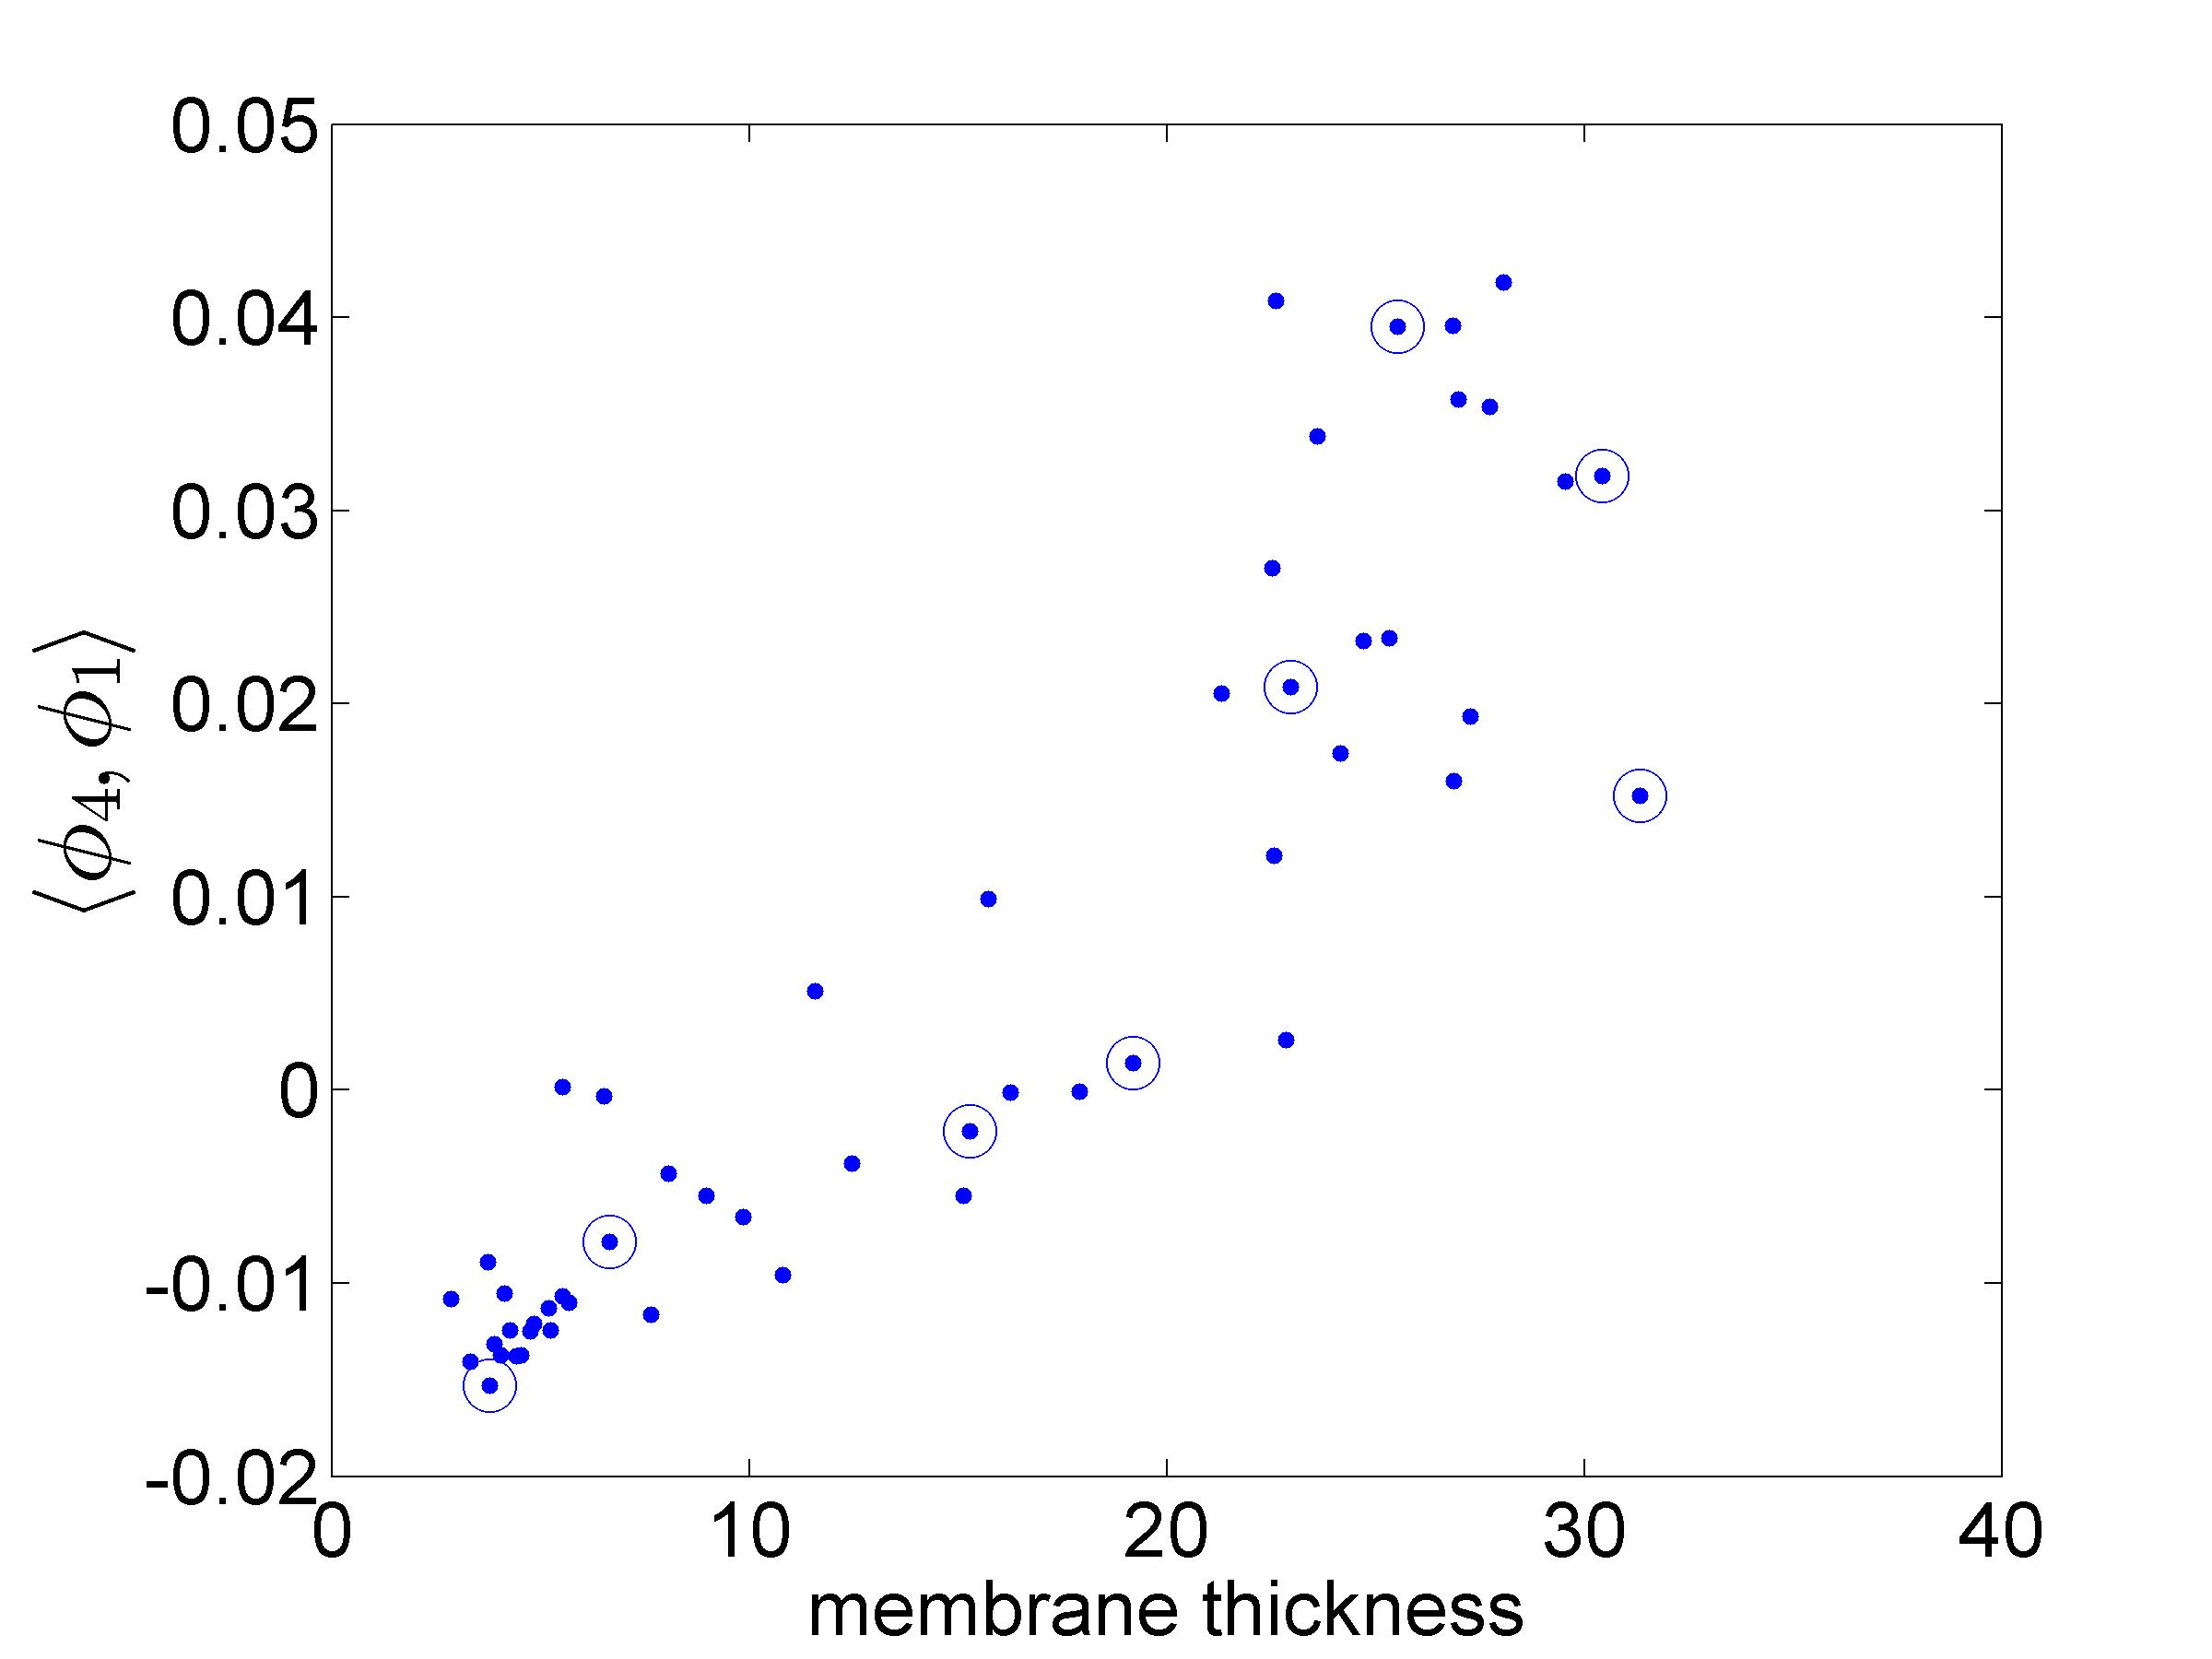
\includegraphics[width=\textwidth]{vdm_2d_time_corr}
\caption{}
\end{subfigure}
\begin{subfigure}{0.5\textwidth}
\foreach \n in {1,9,17,25,30,34,38,43,49}{
\includegraphics[width=0.3\textwidth]{dpERK_vdm_\n}
\hfill}
\caption{}
\end{subfigure}
\caption{{\bf Ordering two-dimensional fluorescent images of dpERK.}
(a) Correlation between the VDM embedding coordinate and the membrane thickness. 
(b) Some representative fluorescent images, aligned  and ordered using the VDM embedding coordinate. }
\label{fig:vdm_image_ordering}
\end{figure}

\subsection*{Two-dimensional dpERK images ordered using diffusion maps and the scattering transform}

An alternative to aligning the data (as in angular synchronization of VDM) is to construct {\em features} that are invariant to the underlying symmetry group, and then compute distances between data points using these features for use in a DMAPS calculation.
%
In our setup, we need features for two-dimensional images that are invariant to translations and rotations of the images.
%
We chose to use the scattering transform \cite{mallat2012group} to construct our invariant features.
%
Not only is this transform invariant to translations and rotations, but it is built on the wavelet transform (which is know to perform well for images), and is also contractive (so that noise and small deformations are not amplified by the transform).

We compute the scattering transform coefficients for each image in our data set.
%
We then perform a DMAPS calculation, using the Euclidean distance between the vectors of scattering transform coefficients as our distance metric.
%
The results are shown in Figure \ref{fig:scattrans_dpERK_ordering}.
%
The ordering is again good; however, using this method, we do not obtain optimal alignments for the images (we only obtain an ordering).

\begin{figure}[H]
\centering
\begin{subfigure}{0.45\textwidth}
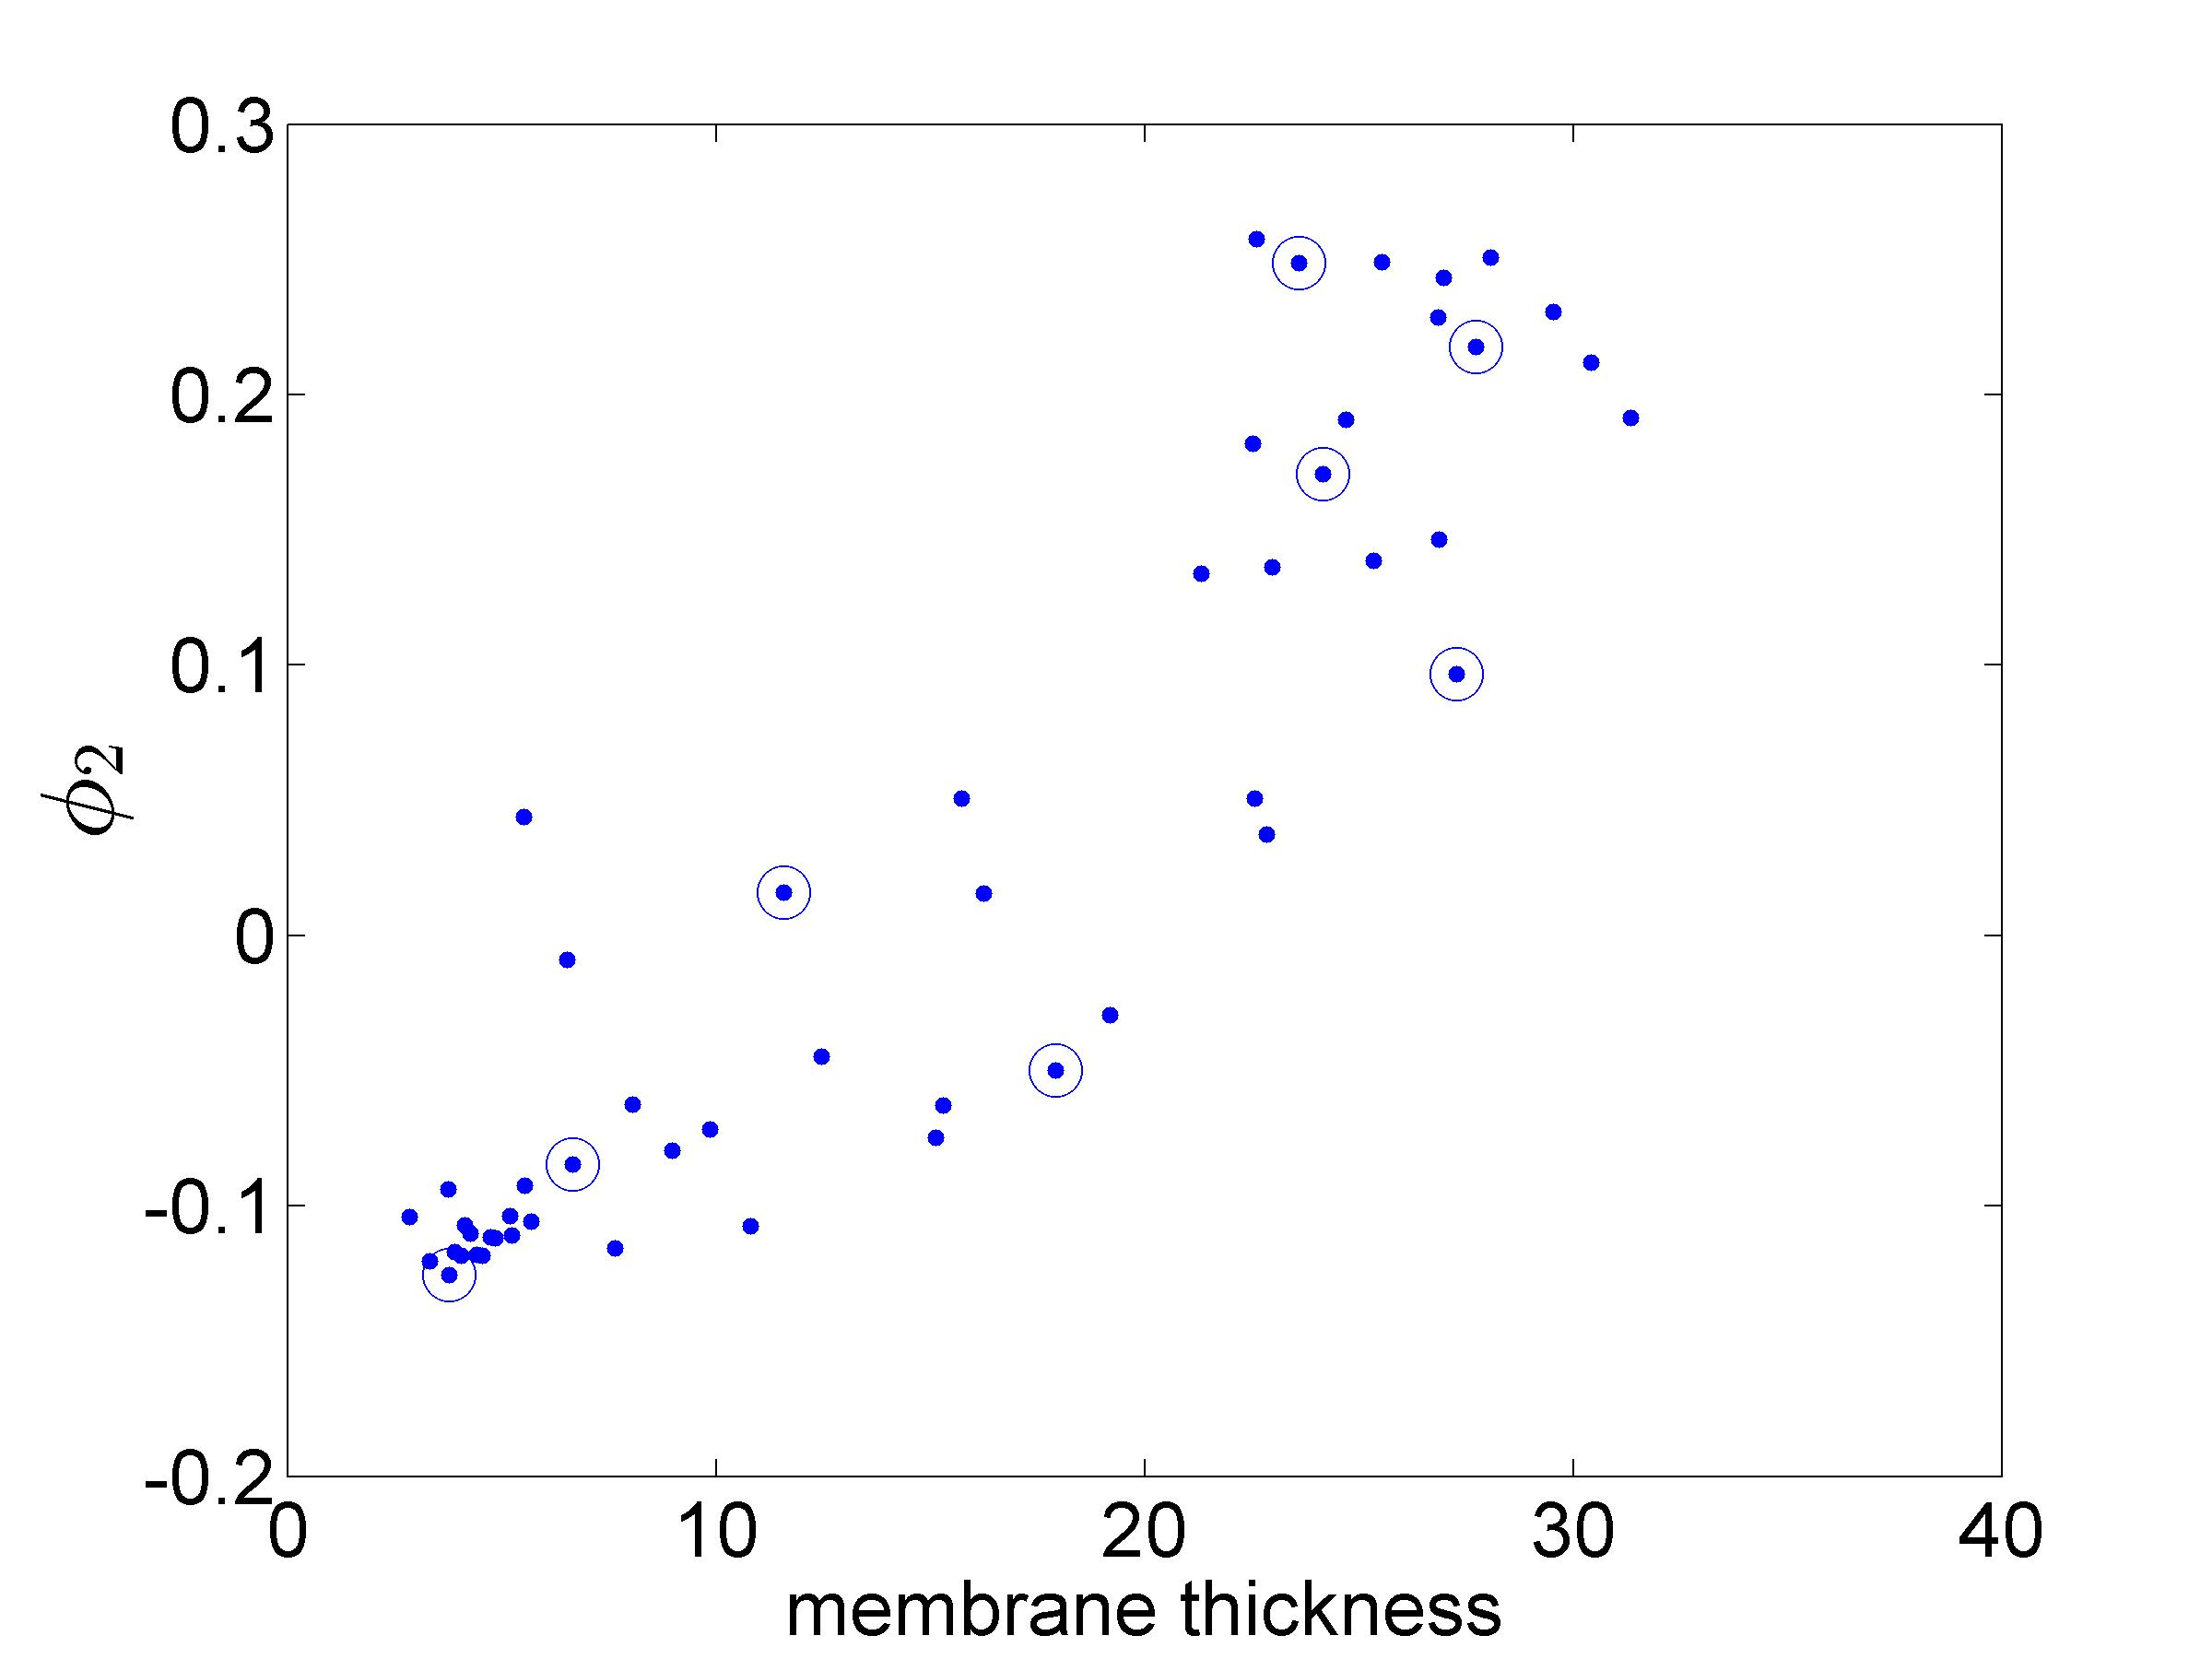
\includegraphics[width=\textwidth]{DMAPS_scat_time_corr}
\caption{}
\end{subfigure}
\begin{subfigure}{0.5\textwidth}
\foreach \n in {1,9,17,25,30,34,38,43,49}{
\includegraphics[width=0.3\textwidth]{dpERK_scat_\n}
\hfill}
\caption{}
\end{subfigure}
\caption{{\bf Ordering two-dimensional fluorescent images of dpERK.}
(a) Correlation between the first (non-trivial) DMAPS embedding coordinate and the membrane thickness. The DMAPS embedding was computed using the translation- and rotation-invariant scattering transform coefficients as ``features'' of the images.
(b) Some representative fluorescent images, ordered using the first (non-trivial) DMAPS embedding coordinate computed from the scattering transform coefficients. }
\label{fig:scattrans_dpERK_ordering}
\end{figure}

\subsection*{Two-dimensional membrane images ordered using diffusion maps and the scattering transform}

\begin{figure}[H]
\centering
\begin{subfigure}{0.45\textwidth}
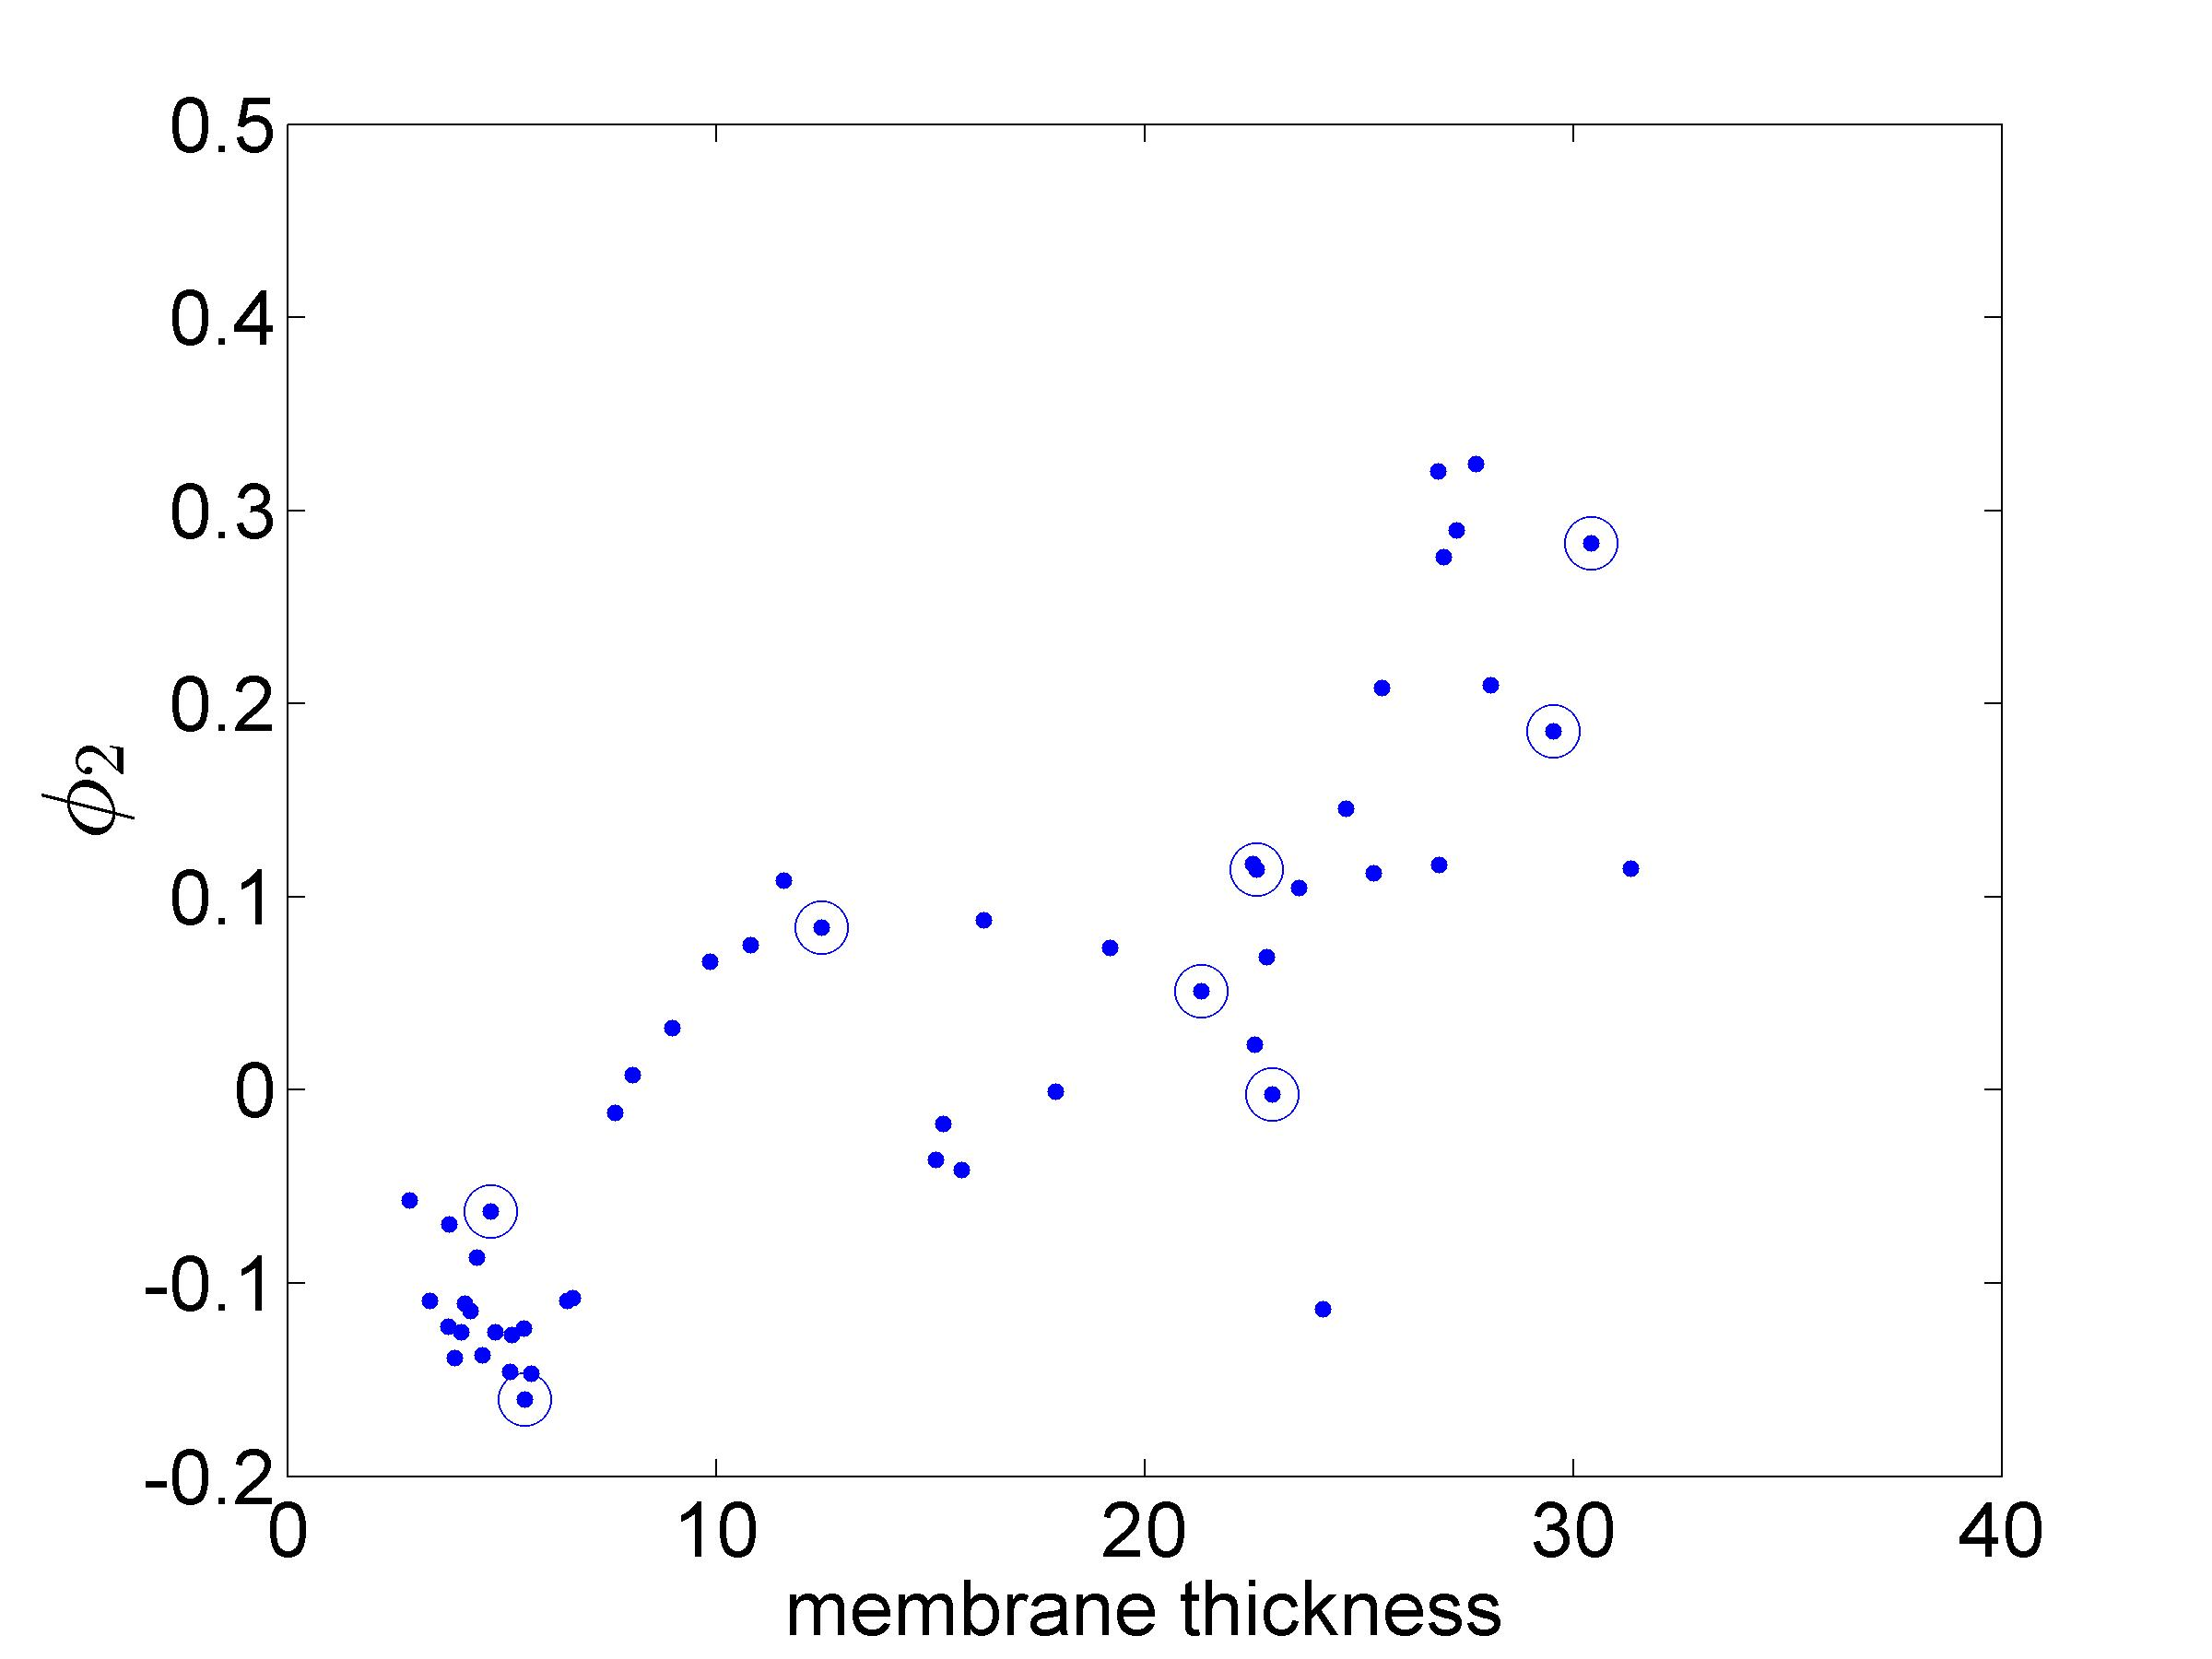
\includegraphics[width=\textwidth]{DMAPS_membrane_scat_time_corr}
\caption{}
\end{subfigure}
\begin{subfigure}{0.5\textwidth}
\foreach \n in {1,9,17,25,30,34,38,43,49}{
\includegraphics[width=0.3\textwidth]{membrane_scat_\n}
\hfill}
\caption{}
\end{subfigure}
\caption{{\bf Ordering two-dimensional fluorescent images of membrane proteins.}
(a) Correlation between the seventh (non-trivial) DMAPS embedding coordinate and the membrane thickness. DMAPS was computed using the translation- and rotation-invariant scattering transform coefficients as ``features'' of the images. The first six non-trivial DMAPS coordinates were found to capture other features of the images, such as  differences in fluorescence intensity within the images.
(b) Some representative fluorescent images, ordered using the seventh (non-trivial) DMAPS embedding coordinate computed from the scattering transform coefficients. }
\label{fig:scattrans_membrane_ordering}
\end{figure}


\section*{Discussion}

We hope that we have illustrated the use of dimensionality reduction techniques in application with underlying symmetries.
%
The work here is intended to provide an overview of the different techniques available, as well as the benefits and shortcomings of each method. 


\begin{table}
	\begin{tabular}{| p{0.3\textwidth} | c | c | p{0.3\textwidth} |}
		\hline 
		Method & Spearman's $\rho$ & Execution Time & Notes About Method \\ 
		\hline 
		PCA on one-dimensional profiles & 0.9244 & $< 1$ second & \\
		\hline 
		DMAPS on one-dimensional profiles & 0.9209 & $< 1$ second & \\
		\hline 
		Angular synchronization + DMAPS on one-dimensional profiles & 0.9164 & $< 1$ second & \\
		\hline 
		VDM on one-dimensional profiles & 0.9232 & $< 1$ second & \\	
		\hline 
		VDM on two-dimensional images & 0.9051  & $325$ seconds & $\mathcal{O}(n^2)$ to compute the pairwise alignments\\
		\hline 	
		Scattering transform + DMAPS on two-dimensional profiles & 0.9011  & $86$ seconds &  $\mathcal{O}(n)$ to compute the scattering transform for each data point \\
		\hline
		Scattering transform + DMAPS on two-dimensional membrane images & 0.8403  & $300$ seconds &  $\mathcal{O}(n)$ to compute the scattering transform for each data point \\
		\hline
	\end{tabular}
\end{table}
% You may title this section "Methods" or "Models".
% "Models" is not a valid title for PLoS ONE authors. However, PLoS ONE
% authors may use "Analysis"
\section*{Materials and Methods}

\subsection*{Experimental Setup}

\subsection*{Image Preprocessing}
The dpERK images we collect from the confocal microscope are subsampled to $100 \times 100$ pixels; the membrane images are subsampled to $200 \times 200$ pixels (due to the finer features in the membrane pictures). 

Because we are only interested in the membrane thickness, we run a simple edge detection algorithm on the membrane images.
%
We use a Laplacian of Gaussians filter \cite{...}, as implemented in the Matlab Image processing toolbox \cite{...}.


\subsection*{Principal Component Analysis}
Principal component analysis (PCA) has been the workhorse dimensionality reduction technique for the past century.
%
PCA finds the optimal planes or hyperplanes on which to project the data in order to maximize the variance of the projected data \cite{shlens2005tutorial}.

Let $X \in \mathbb{R}^{n \times d}$ denote our data set consisting of $n$ points in $d$ dimensions, where $X_{ij}$ denotes the $j^{th}$ dimension of the $i^{th}$ observation. 
%
We first mean-center the data set to produce the matrix $\hat{X}$, where
\begin{equation}
\hat{X}_{ij} = X_{ij} - \frac{1}{n} \sum_{k=1}^n X_{kj}.
\end{equation}
%
The empirical covariance of the data set, $C \in \mathbb{R}^{d \times d}$ is then given by
\begin{equation}
C = X^T X.
\end{equation}
%
We compute the eigenvectors $\psi_1, \dots, \psi_d$ and eigenvalues $\lambda_1, \lambda_2, \dots, \lambda_d$ of $C$, and order them such that $\lambda_1 \ge \lambda_2 \ge \dots \ge \lambda_d$.
%
The principal components of the data set $X$ are given by $\psi_1, \dots, \psi_d$, and the eigenvalues $\lambda_1, \lambda_2, \dots, \lambda_d$ measure the variability captured by the corresponding eigenvector. 
%
If there is a {\em spectral gap} such that the first few eigenvectors capture a significant portion of the variance in our data set, projection onto these first few principal components will retain most features of the data set while reducing the dimensionality.
%
In our setup, we assume that the data is inherently one-dimensional, and that projection onto $\psi_1$ will uncover the correct time ordering of the data.

\subsection*{Diffusion Maps}
Unlike PCA, diffusion maps (DMAPS) is a nonlinear dimensionality reduction technique. 
%
DMAPS aims to uncover the parameterization of data sampled from a nonlinear manifold \cite{coifman2005geometric}.
%
The {\em essential} requirement for DMAPS is an appropriate distance metric $d(x_i, x_j)$ for comparing data points. 
%
This can as simple as the standard Euclidean distance, or a more complex metric (such as a distance between features of the data points) for other data sets.

Given data points $x_1, \dots, x_n \in \mathbb{R}^d$, we fist calculate the matrix $W \in \mathbb{R}^{n \times n}$, where 
\begin{equation}
W_{ij} = \exp \left( -\frac{d^2(x_i, x)j)}{\epsilon} \right)
\end{equation}
and $\epsilon$ is a characteristic distance between data points.
%
$\epsilon$ can be chosen using several techniques (see, for example \cite{coifman2008graph}); in practice, we choose $\epsilon$ to be the median of the pairwise distances between data points.
%
We then compute the diagonal matrix $D$, where $D_{ii} = \sum_{j=1}^{n} W_{ij}$, and the matrix $A = D^{-1} W$. 
%
We calculate the eigenvectors $\phi_1, \phi_2, \dots, \phi_n$ and eigenvalues $\lambda_1, \lambda_2, \dots, \lambda_n$ and order them such that $|\lambda_1| \ge |\lambda_2| \ge \dots \ge |\lambda_n|$. 
%
Because the matrix $A$ is similar to the symmetric matrix $D^{-1/2} W D^{-1/2}$, $A$ is guaranteed to have real eigenvalues and real, orthogonal eigenvectors. 
%
The eigenvectors $\phi_1, \phi_2, \dots, \phi_n$ give the embedding coordinates, such that $\phi_j(i)$ gives the $j^{th}$ embedding coordinate of the $i^{th}$ data point. 
%
Because the matrix $A$ is row-stochastic, $\lambda_1=1$ and $\phi_1$ is a constant vector; the next few eigenvectors give the ``meaningful'' embedding coordinates for the data. 

\subsection*{Angular Synchronization}

When the data set is invariant under an underlying symmetry group (such as translations and/or rotations), we must first factor out the underlying symmetries before doing further analysis.
%
Angular synchronization calculates the optimal alignments for a data set, assuming we have estimates of the optimal alignments between pairs of data points \cite{singer2011angular}. 

Let $x_1, \dots, x_n$ denote the data points that we wish to align under some symmetry group.
%
We will consider the case where the symmetry group is the group of two-dimensional rotations, $SO(2)$; the same construction and ideas hold for other symmetry groups, such as $SO(3)$. 
%
Let $R_{ij} \in SO(2)$ denote the rotation that aligns $x_j$ to $x_i$, so that
\begin{equation}
R_{ij} = \argmin_{R \in SO(2)} \|Rx_j - x_i \|^2.
\end{equation}
%
We seek to find the rotations $R_1, R_2, \dots, R_n \in SO(2)$ such that $R_i R_j^T \approx R_{ij}$, for every pair $i, j$. (CHECK THIS)
%
We would also like to exploit {\em higher-order} consistency relations.
%
For example, for noiseless measurements, $R_{ij} R_{jk} R_{ki} = I$, where $I$ is the identity matrix; therefore, we consider measurements which (almost) satisfy such conditions ``good'' measurements, and those measurements which do not satisfy such conditions as most likely inaccurate.

We define the objective function 
\begin{equation} \label{eqn:angsynch_obj}
\max_{R_1, \dots, R_n \in SO(2)} \sum_{i=1}^{n} \sum_{j=1}^{n} R_i^T R_{ij} R_j.
\end{equation}
%
In general, the solution to \eqref{eqn:angsynch_obj} is not easily computed.

Instead, we relax the problem and allow $R_1, \dots, R_n \in \mathbb{R}^2$.
%
We then define the matrix $H$, which is an $n \times n$ block matrix with $2 \times 2$ blocks (so $H \in \mathbb{R}^{2n \times 2n}$).
%
We then compute the top ``block'' eigenvector of $H$, which we denote $\hat{R} \in \mathbb{R}^{2n \times 2}$. 
%
The solution to the relaxed problem is given by $\hat{R}$, so that the $i^{th}$ rotation is (approximately) $\hat{R}(i) \in \mathbb{R}^{2 \times 2}$.
%
However, because we relaxed the problem to allow our solutions to lie in $\mathbb{R}^{2 \times 2}$, we must project our approximate solution back to $SO(2)$.
%
The optimal rotation is therefore given by $R_i = U_i V_i^T$, where $U_i$ and $V_i$ are the left and right singular vectors of $\hat{R}_i$, respectively. 

\subsection*{Vector Diffusion Maps} 

Angular synchronization assumes that each data point is a replicate measurements of the same underlying configuration, simply corrupted with rotations and some noise.
%
However, in system with an underlying symmetry group {\em as well as} a dynamical process, the data points are not identical modulo symmetries and noise, and we would like to place more emphasis on aligning data points which are dynamically close.

Vector diffusion maps (VDM) couples the symmetry-factoring of angular synchronization with the uncovering of dynamics of diffusion maps \cite{singer2012vector}. 
%
We construct the matrix $A$ as in diffusion maps, and the matrix $H$ as in angular synchronization.
%
We then construct the block matrix $S$, where the blocks of $S$ are defined by
\begin{equation}
S_{ij} = \left\{ \begin{array}{l l} 
A_{ij} H_{ij} & i \ne j \\
0_{2 \times 2} & i = j
\end{array}
\right.
\end{equation}
%
where $A_{ij}$ is the $(i,j)$ entry of $A$, and $H_{ij}$ is the $(i,j)$ block of $H$. 

We then compute the eigenvectors $\phi_1, \dots, \phi_{2n}$ and eigenvalues $\lambda_1, \dots, \lambda_{2n}$ of $S$, and order them such that $|\lambda_1| \ge |\lambda_2| \ge \dots \ge |\lambda_{2n}|$.
%
As in angular synchronization, the first ``block'' eigenvector, i.e. the first two eigenvectors concatenated into a $2 n \times 2$ matrix, gives the optimal rotations. 
%
However, the eigenvectors now also give us embedding coordinates.
%
Let $\phi_j(i)$ denote the $i^{th}$ block of $\phi_j$. 
%
The embedding coordinates are then given by $\langle \phi_j(i), \phi_k(i) \rangle$, where $1 \le j, k, \le 2 n$. 

\subsection*{Scattering Transform}

The scattering transform consists of a wavelet transform of the signal, followed by  the appropriate averaging operator.
%
This transform is applied to the signal itself, as well as to the residual, in order to preserve as much information about the signal itself, while still keeping the transform coefficients translation- and rotation-invariant. 
% 
Furthermore, the scattering transform can be shown to be a contractive operator; therefore, noise and small deformations in the signal are not amplified in the transformation.

\subsection*{Edge detection}
For the membrane images, we are only interested in the location of the edges of the membrane (not other features, such as the intensity of the fluorescent stain).
%
We therefore preprocess the 

\subsection*{Spearman's $\rho$}

Spearman's rank correlation coefficient, or Spearman's $\rho$, measures the monotonicity of a function \cite{...}. 
%
It therefore serves as an appropriate metric for the ``goodness'' of our orderings.
%
Given data points $X_i$ and $Y_i$, we compute the ranks of each data point within the data set, denoted $x_i$ and $y_i$.
%
Spearman's $\rho$ is then defined as the correlation between the ranks
\begin{equation}
\rho = \frac{\sum_i (x_i - \overline{x})(y_i - \overline{y})}{\sqrt{\sum_i (x_i - \overline{x})^2 \sum_i (y_i - \overline{y})^2}}
\end{equation}


% Do NOT remove this, even if you are not including acknowledgments
\section*{Acknowledgments}


%\section*{References}
% The bibtex filename
\bibliography{../../references/references}

\section*{Figure Legends}
%\begin{figure}[!ht]
%\begin{center}
%%\includegraphics[width=4in]{figure_name.2.eps}
%\end{center}
%\caption{
%{\bf Bold the first sentence.}  Rest of figure 2  caption.  Caption
%should be left justified, as specified by the options to the caption
%package.
%}
%\label{Figure_label}
%\end{figure}


\section*{Tables}
%\begin{table}[!ht]
%\caption{
%\bf{Table title}}
%\begin{tabular}{|c|c|c|}
%table information
%\end{tabular}
%\begin{flushleft}Table caption
%\end{flushleft}
%\label{tab:label}
% \end{table}

\end{document}
